\documentclass[12pt,a4paper]{report}

% ─── Packages ────────────────────────────────────────────────────────────────
\usepackage[a4paper, margin=2.5cm]{geometry}
\usepackage[T1]{fontenc}
\usepackage[utf8]{inputenc}
\usepackage{lmodern}
\usepackage{microtype}
\usepackage{xcolor}
\usepackage{graphicx}
\usepackage{booktabs}
\usepackage{longtable}
\usepackage{array}
\usepackage{tabularx}
\usepackage{multirow}
\usepackage{enumitem}
\usepackage{listings}
\usepackage{fancyhdr}
\usepackage{titlesec}
\usepackage{tocloft}
\usepackage{hyperref}
\usepackage{amsmath}
\usepackage{amssymb}
\usepackage{tikz}
\usepackage{pgf}
\usetikzlibrary{shapes.geometric, arrows.meta, positioning, fit, backgrounds, calc}
\usepackage{mdframed}
\usepackage{tcolorbox}
\tcbuselibrary{skins, breakable}
\usepackage{fontawesome5}
\usepackage{setspace}
\usepackage{caption}
\usepackage{subcaption}

% ─── Custom Styles ────────────────────────────────────────────────────────────
\definecolor{primary}{HTML}{1E3A5F}
\definecolor{secondary}{HTML}{2E86AB}
\definecolor{accent}{HTML}{E84855}
\definecolor{success}{HTML}{3BB273}
\definecolor{warning}{HTML}{F4A261}
\definecolor{lightgray}{HTML}{F5F5F5}
\definecolor{darkgray}{HTML}{333333}
\definecolor{codebg}{HTML}{1E1E2E}
\definecolor{codetext}{HTML}{CDD6F4}
\definecolor{p1red}{HTML}{C0392B}

\lstdefinestyle{codestyle}{
  backgroundcolor=\color{codebg},
  basicstyle=\ttfamily\small\color{codetext},
  keywordstyle=\color{accent}\bfseries,
  commentstyle=\color{success}\itshape,
  stringstyle=\color{warning},
  breaklines=true,
  frame=single,
  rulecolor=\color{secondary},
  numbers=left,
  numberstyle=\tiny\color{darkgray},
  tabsize=2,
  showstringspaces=false,
}
\lstset{style=codestyle}

\tcbset{
  testbox/.style={
    enhanced, breakable,
    colback=lightgray, colframe=secondary,
    fonttitle=\bfseries\color{white},
    coltitle=white, attach boxed title to top left,
    boxed title style={colback=secondary, rounded corners},
    rounded corners, drop shadow,
  },
  criticalbox/.style={
    enhanced, breakable,
    colback=red!5, colframe=p1red,
    fonttitle=\bfseries\color{white},
    coltitle=white, attach boxed title to top left,
    boxed title style={colback=p1red, rounded corners},
    rounded corners,
  },
  infobox/.style={
    enhanced, breakable,
    colback=blue!5, colframe=primary,
    fonttitle=\bfseries\color{white},
    coltitle=white, attach boxed title to top left,
    boxed title style={colback=primary, rounded corners},
    rounded corners,
  },
  warningbox/.style={
    enhanced, breakable,
    colback=orange!8, colframe=warning,
    fonttitle=\bfseries\color{white},
    coltitle=white, attach boxed title to top left,
    boxed title style={colback=warning, rounded corners},
    rounded corners,
  },
}

\tikzset{
  startstop/.style={
    rectangle, rounded corners=8pt,
    minimum width=3cm, minimum height=0.9cm,
    text centered, draw=primary, very thick,
    fill=primary!15, font=\small\bfseries,
  },
  process/.style={
    rectangle,
    minimum width=3.5cm, minimum height=0.9cm,
    text centered, draw=secondary, thick,
    fill=secondary!10, font=\small,
  },
  decision/.style={
    diamond, aspect=2.2,
    minimum width=3.5cm, minimum height=0.9cm,
    text centered, draw=accent, thick,
    fill=accent!10, font=\small,
  },
  io/.style={
    trapezium, trapezium left angle=70, trapezium right angle=110,
    minimum width=3cm, minimum height=0.9cm,
    text centered, draw=success, thick,
    fill=success!10, font=\small,
  },
  terminal/.style={
    rectangle, rounded corners=15pt,
    minimum width=2.5cm, minimum height=0.9cm,
    text centered, draw=accent, very thick,
    fill=accent!20, font=\small\bfseries,
  },
  arrow/.style={-{Stealth[length=6pt]}, thick, color=darkgray},
  yes/.style={font=\small\color{success}\bfseries},
  no/.style={font=\small\color{accent}\bfseries},
}
\newcommand{\pone}{\textbf{\color{p1red}P1}}
\newcommand{\ptwo}{\textbf{\color{p2orange}P2}}
\newcommand{\pthree}{\textbf{\color{p3blue}P3}}
\newcommand{\pfour}{\textbf{\color{p4green}P4}}

\setlength{\parskip}{6pt}
\setlength{\parindent}{0pt}

\begin{document}

\begin{titlepage}
\begin{center}
    \vspace*{1.5cm}
    
    {\fontsize{20}{24}\selectfont \textbf{Indian Institute of Information Technology, Vadodara}}\\[2cm]
    
    {\fontsize{24}{28}\selectfont \textbf{INVENTORY \& SUPPLY CHAIN MANAGEMENT SYSTEM}}\\[2cm]
    
    {\Large \textbf{A Project Report}}\\[3cm]
    
    {\large \textbf{Submitted by:}}\\[0.5cm]
    {\large Ashay Gupta (202451024)}\\[0.2cm]
    {\large Avni Singhal (202451026)}\\[0.2cm]
    {\large Nandish Chauhan (202451040)}\\[0.2cm]
    {\large Arpit Maheshwari (202451022)}\\[3cm]
    
    {\large \textbf{Course: }Software Engineering Lab (CS 264)}\\[0.5cm]
    
    {\large \textbf{Submitted to: }Dr. Pooja Mishra}\\[2cm]
    
\end{center}
\end{titlepage}


\chapter*{Abstract}
\addcontentsline{toc}{chapter}{Abstract}
This project presents the design and implementation of a web-based Inventory and Supply Chain Management System (Stockly) developed to simplify and modernize the process of inventory tracking, order management, and supply chain operations. Traditional inventory methods are often time-consuming, error-prone, and inefficient. The proposed system provides a secure and automated digital solution that enhances accuracy, transparency, and ease of use.

The system is built with a role-based architecture consisting of multiple users including Admin, Supplier, Retailer, and Client. Users can manage products, coordinate stock allocations across various warehouses, generate comprehensive invoices, and manage orders with integrated stock reservation logic. 

The application utilizes Next.js for a robust frontend and scalable API backend alongside MongoDB and Prisma ORM for efficient data handling and instant synchronization. 

Key features of the system include role-based access control, real-time inventory tracking, intelligent demand forecasting, automated email notifications (via Brevo), and an intuitive dashboard interface. This project demonstrates the effective use of modern web technologies and cloud-based systems to build a reliable and scalable supply chain solution.
\newpage


\chapter*{Acknowledgement}
\addcontentsline{toc}{chapter}{Acknowledgement}
We would like to express our sincere gratitude to our subject teacher and project guide, Dr. Pooja Mishra, for her continuous support, valuable guidance, and encouragement throughout the development of this project. Her insights and suggestions greatly helped us in improving the quality of our work.

We also extend our thanks to the Teaching Assistants (TAs) for their assistance, timely feedback, and support during the course of this project.

Finally, we would like to thank our institution for providing us with the necessary resources and environment to successfully complete this project.\\[2cm]

\noindent
\textbf{Team Members} \hfill \textbf{Signature:.....................................}
\newpage

\tableofcontents
\newpage

\chapter{Introduction}
% ═════════════════════════════════════════════════════════════════════════════

\section{Project Overview}

Stockly is a production-grade, full-stack inventory and supply chain management system developed to address the operational challenges faced by small-to-medium enterprises (SMEs) engaged in product distribution, warehousing, and retail. The platform consolidates product management, order processing, invoice generation, supplier coordination, warehouse tracking, customer support, and business analytics into a single, cohesive web application accessible from any modern browser.

The system is publicly accessible at \url{https://stockly-inventory.vercel.app} and is open-sourced under the MIT license. It is built with a technology stack chosen for developer productivity, runtime performance, and long-term maintainability.

\begin{tcolorbox}[infobox,title={Three-Role Architecture}]
Unlike traditional inventory tools that serve a single user type, Stockly provides \textbf{three fully distinct role-based experiences} within a single application:
\begin{itemize}[leftmargin=1.5em]
  \item \textbf{Admin (Store Owner):} Complete system control --- products, orders, invoices, warehouses, users, analytics, and portal oversight of both clients and suppliers.
  \item \textbf{Supplier:} Scoped view of their own products, associated orders, revenue metrics, low-stock alerts, and support tickets.
  \item \textbf{Client:} A consumer-facing portal for browsing the product catalog, placing orders, paying invoices via Stripe, and managing support requests.
\end{itemize}
\end{tcolorbox}

The application follows the \textbf{Next.js 16 App Router} paradigm, where both the frontend (React Server Components and Client Components) and the backend (API Route Handlers) coexist within the same codebase. This architecture eliminates the need for a separate backend server, simplifies deployment, and enables efficient server-side rendering (SSR) and static generation (SSG) where appropriate.

\section{Purpose}

The primary purpose of Stockly is to eliminate the inefficiencies of manual or spreadsheet-based inventory management by providing a unified digital platform with the following capabilities:

\begin{enumerate}[leftmargin=1.5em]
  \item \textbf{Real-time stock visibility:} Automatic computation of available stock using the formula $\text{availableStock} = \text{quantity} - \text{reservedQuantity}$, with status labels (available, stock low, out of stock) updated dynamically.
  \item \textbf{Automated order-to-invoice workflows:} Orders automatically trigger invoice creation, status tracking, and payment collection, reducing administrative overhead and human error.
  \item \textbf{Financial integrity:} Invoice calculations use \texttt{Math.max(0, subtotal + tax + shipping - discount)} to prevent negative totals, and nullish coalescing (\texttt{??}) ensures explicit zero values are respected over fallback values.
  \item \textbf{Demand forecasting:} Statistical analysis of historical sales data (moving averages, standard deviation, linear regression) predicts future stock requirements and generates reorder recommendations.
  \item \textbf{Multi-role access control:} JWT-based authentication with role-based query filtering ensures data isolation between clients, suppliers, and administrators.
  \item \textbf{Operational transparency:} Comprehensive audit logs, activity history, and import history provide a full trail of all system changes.
  \item \textbf{Extensible integrations:} The system is designed so the core application runs with only three environment variables, with all integrations (Stripe, Shippo, Brevo, etc.) being optional and gracefully degraded when not configured.
\end{enumerate}

\section{Scope}

The scope of this project encompasses the following functional domains:

\begin{center}
\begin{tabularx}{\textwidth}{lX}
  \toprule
  \textbf{Domain} & \textbf{Scope Description} \\
  \midrule
  Product Management    & Full CRUD with SKU, categories, suppliers, stock levels, status, QR codes, CSV/Excel import/export, image upload via ImageKit \\
  Order Management      & Multi-item orders with tax/shipping/discount, 6-state status machine, stock reservation/release logic \\
  Invoice Management    & Auto-generated invoices linked 1:1 to orders, PDF export, email delivery, Stripe payment links, overdue tracking \\
  Warehouse Management  & CRUD for warehouses, stock allocation per warehouse, stock transfer between warehouses \\
  User Management       & Admin-controlled user CRUD, role assignment (admin/supplier/client/user/retailer), activity tracking \\
  Supplier Portal       & Supplier-scoped dashboard with product/order/revenue views, low-stock alerts \\
  Client Portal         & Consumer catalog with browse/filter, order placement, invoice payment, support tickets \\
  Analytics             & Revenue charts, order trends, category breakdowns, demand forecasting, AI insights via OpenRouter \\
  Support System        & Ticket creation, reply threads, priority/status management, role-scoped visibility \\
  Product Reviews       & Customer reviews with admin moderation (approve/reject), eligibility verification by order \\
  Notifications         & In-app notification system, optional email via Brevo with QStash queue \\
  API Infrastructure    & RESTful API with JWT auth, Zod validation, rate limiting, Redis caching, OpenAPI spec \\
  \bottomrule
\end{tabularx}
\end{center}

\section{Issues and Challenges}

\begin{tcolorbox}[warningbox,title={Known Issues and Technical Challenges}]
\begin{enumerate}[leftmargin=1.5em]
  \item \textbf{Race Condition in Order Number Generation:} \texttt{generateOrderNumber()} uses a non-atomic count-based sequence. Under high concurrency, duplicate sequence numbers are theoretically possible. Mitigation: use a distributed atomic counter (e.g., Redis \texttt{INCR}) in production.
  \item \textbf{Invoice Number Collision Risk:} \texttt{generateInvoiceNumber()} uses a random 4-digit suffix with a while-loop uniqueness check. Collision probability is 1/9000 per attempt, but the loop is unbounded under extreme load.
  \item \textbf{JWT Secret Default Fallback:} If \texttt{JWT\_SECRET} is not set, the system defaults to \texttt{"your\_jwt\_secret"} --- a critical security vulnerability in production.
  \item \textbf{Non-Atomic Stock Reservation:} Stock reservation during order creation involves multiple sequential Prisma updates. A server crash between order creation and stock reservation could leave stock in an inconsistent state. MongoDB transactions should be used for full atomicity.
  \item \textbf{Forecasting Data Dependency:} The demand forecasting engine requires at least 7 days of historical sales data for trend analysis. Products with fewer data points receive a default ``stable'' classification.
  \item \textbf{Optional Integration Degradation:} When Stripe, Shippo, Brevo, or Redis are not configured, the system falls back to mock/disabled behavior, which may not be immediately obvious to end users without proper UI indicators.
\end{enumerate}
\end{tcolorbox}

\section{Technology Stack Summary}

\begin{center}
\begin{tabularx}{\textwidth}{llX}
  \toprule
  \textbf{Layer} & \textbf{Technology} & \textbf{Purpose} \\
  \midrule
  Framework    & Next.js 16 (App Router) & SSR, SSG, API routes, file-based routing \\
  Language     & TypeScript 5 (strict)   & End-to-end type safety \\
  Database     & MongoDB + Prisma ORM 6.4 & Document storage, schema validation, query builder \\
  Auth         & JWT + bcryptjs           & Stateless session management, password hashing \\
  State (server) & TanStack Query         & Server state, caching, background refetch \\
  State (client) & Zustand                & Lightweight client-side state \\
  UI           & Tailwind CSS + shadcn/ui & Utility-first styling, accessible component primitives \\
  Forms        & React Hook Form + Zod    & Form management and schema validation \\
  Payments     & Stripe                   & Checkout sessions, payment intents, webhooks \\
  Shipping     & Shippo                   & Label generation, rate calculation, tracking \\
  Email        & Brevo + QStash           & Transactional email, background job queue \\
  Images       & ImageKit                 & CDN-backed image upload and transformation \\
  Cache        & Upstash Redis            & API response caching, rate limiting \\
  Monitoring   & Sentry                   & Error tracking and performance monitoring \\
  AI           & OpenRouter               & AI-powered business insights \\
  \bottomrule
\end{tabularx}
\end{center}

% ═════════════════════════════════════════════════════════════════════════════

\chapter{Requirement Analysis}
% ═════════════════════════════════════════════════════════════════════════════

\section{Software Requirements Specification (SRS)}

This chapter presents the formal Software Requirements Specification for Stockly. Requirements are classified as Functional (FR) or Non-Functional (NFR) and prioritized using the MoSCoW method (Must Have, Should Have, Could Have, Won't Have).

\section{Stakeholders and User Roles}

\begin{center}
\begin{tabularx}{\textwidth}{llX}
  \toprule
  \textbf{Stakeholder} & \textbf{Role} & \textbf{Primary Concerns} \\
  \midrule
  Store Owner   & Admin    & Full system control, analytics, user management, financial oversight \\
  Product Supplier & Supplier & Own product visibility, order tracking, revenue reporting \\
  Customer      & Client   & Product browsing, order placement, invoice payment, support \\
  System Admin  & Admin    & User management, system configuration, audit logs \\
  Developer     & Internal & API access, integration management, monitoring \\
  \bottomrule
\end{tabularx}
\end{center}

\section{Functional Requirements}

\subsection{Authentication and User Management}

\begin{tcolorbox}[reqbox,title={FR-AUTH: Authentication Requirements}]
\begin{itemize}[leftmargin=1.5em]
  \item \req{FR-AUTH-01} The system SHALL allow users to register with email, name, and password. Passwords must be hashed using bcrypt with a minimum of 10 salt rounds before storage.
  \item \req{FR-AUTH-02} The system SHALL authenticate users via email/password and issue a signed JWT token stored as an \texttt{httpOnly} cookie named \texttt{session\_id} with a 1-hour expiry.
  \item \req{FR-AUTH-03} The system SHALL support Google OAuth 2.0 as an alternative authentication method.
  \item \req{FR-AUTH-04} The system SHALL validate JWT tokens on every protected API request. Expired, malformed, or tampered tokens SHALL result in a 401 Unauthorized response.
  \item \req{FR-AUTH-05} The system SHALL support session logout by clearing the \texttt{session\_id} cookie.
  \item \req{FR-AUTH-06} The system SHALL enforce role-based access control. Users with insufficient roles SHALL receive a 403 Forbidden response.
  \item \req{FR-AUTH-07} Admin users SHALL be able to create, update, deactivate, and delete user accounts and assign roles.
\end{itemize}
\end{tcolorbox}

\subsection{Product Management}

\begin{tcolorbox}[reqbox,title={FR-PROD: Product Requirements}]
\begin{itemize}[leftmargin=1.5em]
  \item \req{FR-PROD-01} The system SHALL support full CRUD operations for products with fields: name, SKU (unique), price, quantity, reservedQuantity, status, categoryId, supplierId, description, imageUrl, qrCodeUrl, and expirationDate.
  \item \req{FR-PROD-02} Product status SHALL be automatically computed: \texttt{available} (quantity $>$ threshold), \texttt{stock\_low} (quantity $\leq$ threshold), \texttt{out\_of\_stock} (quantity $= 0$).
  \item \req{FR-PROD-03} The system SHALL generate QR codes for products and store them via ImageKit.
  \item \req{FR-PROD-04} The system SHALL support bulk product import from CSV and Excel files, with per-row error reporting and import history tracking.
  \item \req{FR-PROD-05} The system SHALL support product image upload via ImageKit with automatic cleanup of old images on update.
  \item \req{FR-PROD-06} SKU values SHALL be globally unique across all products.
  \item \req{FR-PROD-07} The system SHALL support product filtering by category, supplier, status, and price range, with pagination.
\end{itemize}
\end{tcolorbox}

\subsection{Order Management}

\begin{tcolorbox}[reqbox,title={FR-ORD: Order Requirements}]
\begin{itemize}[leftmargin=1.5em]
  \item \req{FR-ORD-01} The system SHALL support creation of orders with multiple line items, each capturing productId, quantity, unit price (snapshot), and subtotal.
  \item \req{FR-ORD-02} On order creation, the system SHALL verify available stock ($\text{quantity} - \text{reservedQuantity} \geq \text{requestedQuantity}$) for each item and reject the order if any item has insufficient stock.
  \item \req{FR-ORD-03} On successful order creation, the system SHALL increment \texttt{reservedQuantity} for each ordered product.
  \item \req{FR-ORD-04} The order status state machine SHALL support the following transitions: \texttt{pending} $\to$ \texttt{confirmed} $\to$ \texttt{processing} $\to$ \texttt{shipped} $\to$ \texttt{delivered}, with cancellation possible from any non-delivered state.
  \item \req{FR-ORD-05} On order confirmation/payment, the system SHALL decrement both \texttt{quantity} and \texttt{reservedQuantity} for each ordered product.
  \item \req{FR-ORD-06} On order cancellation from a pending state, the system SHALL decrement \texttt{reservedQuantity} (releasing the reservation). On cancellation from confirmed/processing/shipped, the system SHALL increment \texttt{quantity} (restoring stock).
  \item \req{FR-ORD-07} Order totals SHALL be computed as: $\text{total} = \text{subtotal} + \text{tax} + \text{shipping} - \text{discount}$.
  \item \req{FR-ORD-08} The system SHALL generate unique order numbers in the format \texttt{ORD-YYYY-MMDD-HHMMSS-NNNN}.
  \item \req{FR-ORD-09} Clients SHALL only see their own orders. Suppliers SHALL only see orders containing their products. Admins SHALL see all orders.
\end{itemize}
\end{tcolorbox}

\subsection{Invoice Management}

\begin{tcolorbox}[reqbox,title={FR-INV: Invoice Requirements}]
\begin{itemize}[leftmargin=1.5em]
  \item \req{FR-INV-01} Each order SHALL have at most one invoice (enforced by a unique constraint on \texttt{orderId}).
  \item \req{FR-INV-02} Invoice numbers SHALL be unique and generated in the format \texttt{INV-YYYYMMDD-HHMMSS-XXXX} with collision detection.
  \item \req{FR-INV-03} Invoice totals SHALL use \texttt{Math.max(0, subtotal + tax + shipping - discount)} to prevent negative totals.
  \item \req{FR-INV-04} Tax, shipping, and discount values SHALL use nullish coalescing (\texttt{??}) to respect explicit zero values from the request over order defaults.
  \item \req{FR-INV-05} New invoices SHALL always start with \texttt{status = "draft"} and \texttt{amountPaid = 0}.
  \item \req{FR-INV-06} The system SHALL support invoice PDF generation and email delivery to clients.
  \item \req{FR-INV-07} The system SHALL generate Stripe payment links for invoices and process payments via Stripe Checkout.
  \item \req{FR-INV-08} The system SHALL send automated overdue invoice reminders via a scheduled endpoint protected by \texttt{INTERNAL\_API\_KEY}.
\end{itemize}
\end{tcolorbox}

\subsection{Warehouse and Stock Allocation}

\begin{tcolorbox}[reqbox,title={FR-WH: Warehouse Requirements}]
\begin{itemize}[leftmargin=1.5em]
  \item \req{FR-WH-01} The system SHALL support CRUD operations for warehouses with fields: name, address, type, and status.
  \item \req{FR-WH-02} The system SHALL support stock allocation records linking products to warehouses with per-warehouse quantity and reservedQuantity.
  \item \req{FR-WH-03} The system SHALL support stock transfer operations between warehouses with status tracking (pending, completed, cancelled).
  \item \req{FR-WH-04} A product-warehouse combination SHALL be unique (enforced by a composite unique index on \texttt{[productId, warehouseId]}).
\end{itemize}
\end{tcolorbox}

\subsection{Analytics and Forecasting}

\begin{tcolorbox}[reqbox,title={FR-ANALYTICS: Analytics Requirements}]
\begin{itemize}[leftmargin=1.5em]
  \item \req{FR-ANA-01} The admin dashboard SHALL display: total products, orders, invoices, revenue, low-stock count, and recent activity.
  \item \req{FR-ANA-02} The business insights page SHALL display revenue trends, order volume charts, category breakdowns, and supplier performance metrics.
  \item \req{FR-ANA-03} The demand forecasting engine SHALL analyze the last 30 days of sales data and forecast the next 14 days using weighted moving averages.
  \item \req{FR-ANA-04} The forecasting engine SHALL detect sales anomalies using z-score analysis with a threshold of 2.0 standard deviations.
  \item \req{FR-ANA-05} The system SHALL generate reorder recommendations: \texttt{urgent} ($\leq 7$ days until stockout), \texttt{soon} ($\leq 14$ days), \texttt{overstocked} ($> 90$ days), \texttt{normal} (otherwise).
  \item \req{FR-ANA-06} The system SHALL compute a confidence score (0--100) for each forecast based on data volume and coefficient of variation.
  \item \req{FR-ANA-07} The system SHALL optionally provide AI-generated business insights via OpenRouter when \texttt{OPENROUTER\_API\_KEY} is configured.
\end{itemize}
\end{tcolorbox}

\subsection{Support Tickets and Product Reviews}

\begin{tcolorbox}[reqbox,title={FR-SUPPORT: Support and Review Requirements}]
\begin{itemize}[leftmargin=1.5em]
  \item \req{FR-SUP-01} Any authenticated user SHALL be able to create support tickets with subject, description, priority (low/medium/high/urgent), and optional links to products, orders, or suppliers.
  \item \req{FR-SUP-02} Support tickets SHALL support threaded replies from any authenticated user.
  \item \req{FR-SUP-03} Ticket status SHALL follow: \texttt{open} $\to$ \texttt{in\_progress} $\to$ \texttt{resolved} $\to$ \texttt{closed}.
  \item \req{FR-REV-01} Clients SHALL be able to submit product reviews (rating 1--5, comment) only for products they have ordered and received.
  \item \req{FR-REV-02} Product reviews SHALL require admin approval before being publicly visible.
  \item \req{FR-REV-03} The system SHALL enforce one review per order-product combination.
\end{itemize}
\end{tcolorbox}

\section{Non-Functional Requirements}

\begin{center}
\begin{longtable}{lp{4cm}p{8cm}}
  \toprule
  \textbf{ID} & \textbf{Category} & \textbf{Requirement} \\
  \midrule
  \endhead
  NFR-01 & Performance      & API responses SHALL complete within 500ms for 95\% of requests under normal load. Dashboard aggregation queries SHALL complete within 2 seconds. \\
  NFR-02 & Security         & All passwords SHALL be hashed with bcrypt (min 10 rounds). JWT tokens SHALL expire after 1 hour. All API routes SHALL validate authentication before processing. \\
  NFR-03 & Security         & The \texttt{session\_id} cookie SHALL be \texttt{httpOnly}, \texttt{Secure} (in production), and \texttt{SameSite=Strict} to prevent XSS and CSRF attacks. \\
  NFR-04 & Rate Limiting    & API endpoints SHALL enforce rate limiting via Upstash Redis. Exceeded limits SHALL return HTTP 429 with a \texttt{Retry-After} header. \\
  NFR-05 & Availability     & The system SHALL target 99.9\% uptime when deployed on Vercel with MongoDB Atlas. \\
  NFR-06 & Scalability      & The caching layer (Upstash Redis) SHALL reduce database load by caching frequently accessed resources (products, orders, dashboard stats) with appropriate TTLs. \\
  NFR-07 & Maintainability  & All API routes SHALL use Zod schemas for input validation. Validation errors SHALL return structured error messages with field-level details. \\
  NFR-08 & Auditability     & All create, update, and delete operations on core entities SHALL be recorded in the \texttt{AuditLog} collection with userId, action, entityType, entityId, and timestamp. \\
  NFR-09 & Accessibility    & The UI SHALL follow WCAG 2.1 AA guidelines using accessible shadcn/ui components built on Radix UI primitives. \\
  NFR-10 & Portability      & The system SHALL run on any Node.js 18+ environment with only three required environment variables (\texttt{DATABASE\_URL}, \texttt{JWT\_SECRET}, \texttt{NEXT\_PUBLIC\_API\_URL}). \\
  NFR-11 & Observability    & When Sentry is configured, all unhandled exceptions SHALL be captured with full stack traces and user context. \\
  NFR-12 & Data Integrity   & MongoDB unique indexes SHALL enforce uniqueness on \texttt{Product.sku}, \texttt{Invoice.invoiceNumber}, \texttt{Order.orderNumber}, \texttt{User.email}, and \texttt{StockAllocation[productId, warehouseId]}. \\
  \bottomrule
\end{longtable}
\end{center}

\section{Use Cases}

\subsection{Use Case: Place an Order (Client)}

\begin{tcolorbox}[reqbox,title={UC-01: Place Order}]
\textbf{Actor:} Client \\
\textbf{Precondition:} Client is authenticated. Products are in stock. \\
\textbf{Main Flow:}
\begin{enumerate}[leftmargin=1.5em]
  \item Client browses the product catalog and selects items.
  \item Client adds items to the order with desired quantities.
  \item System validates stock availability for each item.
  \item System creates the order, reserves stock, and generates an order number.
  \item System creates a linked invoice in \texttt{draft} status.
  \item Client receives order confirmation with invoice details.
\end{enumerate}
\textbf{Alternate Flow (Insufficient Stock):} System returns an error message specifying the product and available quantity. Order is not created. No stock is reserved. \\
\textbf{Postcondition:} Order exists in \texttt{pending} status. \texttt{reservedQuantity} incremented for each ordered product.
\end{tcolorbox}

\subsection{Use Case: Process Payment (Client)}

\begin{tcolorbox}[reqbox,title={UC-02: Pay Invoice via Stripe}]
\textbf{Actor:} Client \\
\textbf{Precondition:} Invoice exists in \texttt{sent} or \texttt{draft} status. Stripe is configured. \\
\textbf{Main Flow:}
\begin{enumerate}[leftmargin=1.5em]
  \item Client navigates to invoice detail page.
  \item Client clicks ``Pay Now'' button.
  \item System creates a Stripe Checkout session with the invoice amount.
  \item Client is redirected to Stripe's hosted payment page.
  \item Client completes payment.
  \item Stripe sends a \texttt{checkout.session.completed} webhook to \texttt{/api/payments/webhook}.
  \item System updates invoice status to \texttt{paid}, sets \texttt{paidAt}, and updates order \texttt{paymentStatus} to \texttt{paid}.
\end{enumerate}
\textbf{Postcondition:} Invoice status is \texttt{paid}. Order payment status is \texttt{paid}.
\end{tcolorbox}

\subsection{Use Case: Manage Inventory (Admin)}

\begin{tcolorbox}[reqbox,title={UC-03: Admin Inventory Management}]
\textbf{Actor:} Admin \\
\textbf{Main Flow:}
\begin{enumerate}[leftmargin=1.5em]
  \item Admin navigates to the Products section.
  \item Admin can create, edit, or delete products.
  \item Admin can import products in bulk via CSV/Excel upload.
  \item System validates each row, imports valid rows, and reports errors for invalid rows.
  \item Import history is recorded with success/failure counts.
  \item Admin can view low-stock products and trigger reorder workflows.
\end{enumerate}
\end{tcolorbox}

% ═════════════════════════════════════════════════════════════════════════════

\chapter{Design and Architecture}
% ═════════════════════════════════════════════════════════════════════════════

\section{System Architecture Overview}

Stockly follows a \textbf{monolithic full-stack architecture} using the Next.js 16 App Router, where the frontend and backend coexist in a single deployable unit. This approach simplifies deployment, eliminates cross-origin complexity, and enables efficient server-side rendering.

\begin{figure}[h!]
\centering
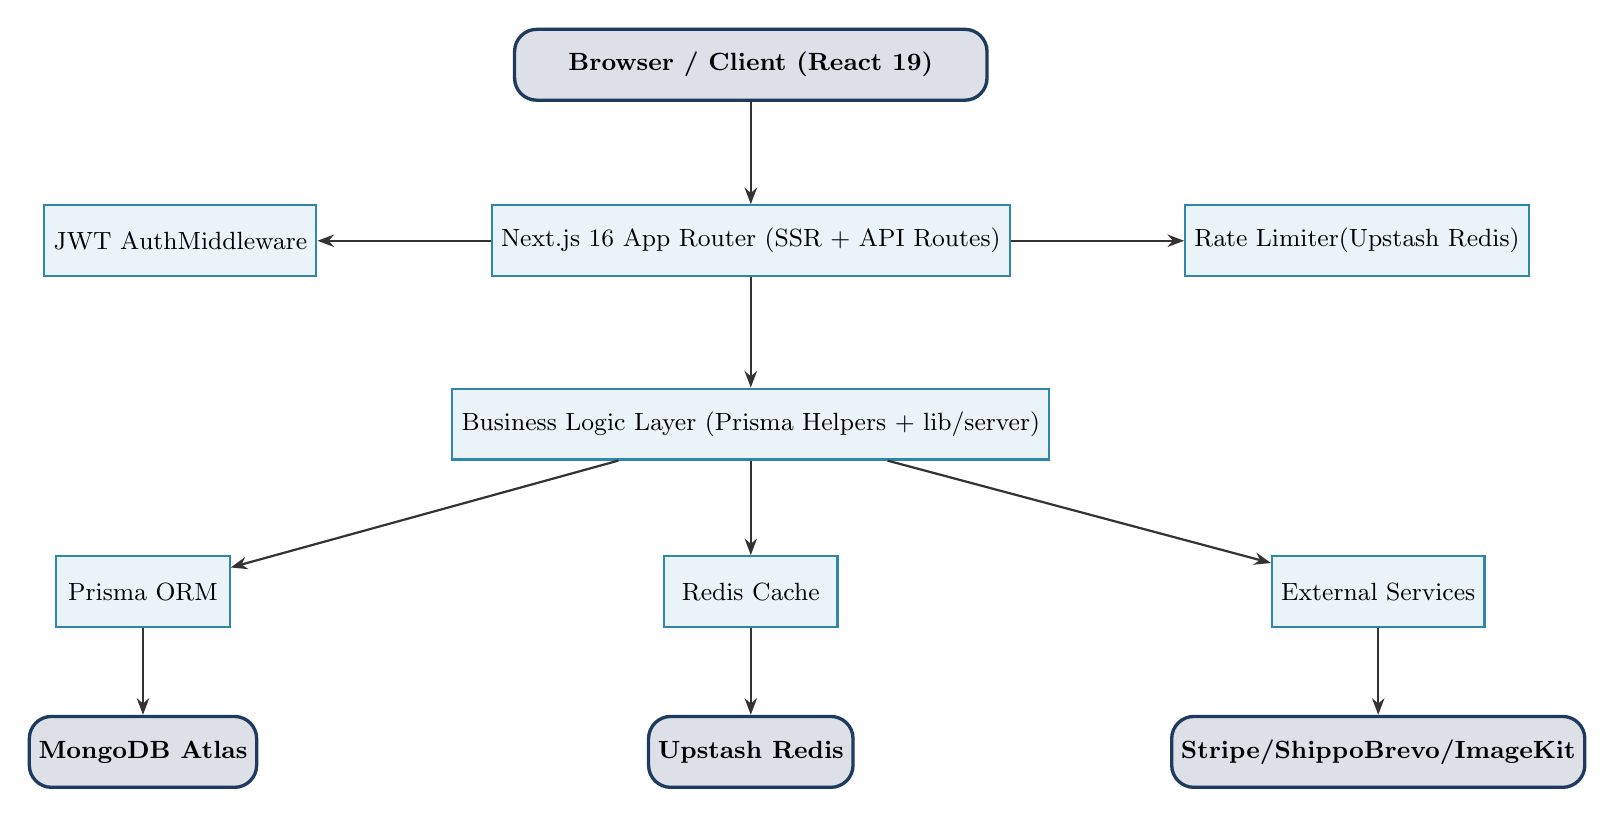
\begin{tikzpicture}[node distance=1.3cm,every node/.style={font=\small}]
  \node[startstop,minimum width=6cm] (browser) {Browser / Client (React 19)};
  \node[process,minimum width=6cm,below=of browser] (nextjs) {Next.js 16 App Router (SSR + API Routes)};
  \node[process,minimum width=3cm,right=2.2cm of nextjs] (ratelimit) {Rate Limiter\\(Upstash Redis)};
  \node[process,minimum width=3cm,left=2.2cm of nextjs] (auth) {JWT Auth\\Middleware};
  \node[process,minimum width=6cm,below=1.4cm of nextjs] (bizlogic) {Business Logic Layer (Prisma Helpers + lib/server)};
  \node[process,minimum width=2.2cm,below left=1.2cm and 2.8cm of bizlogic] (prisma) {Prisma ORM};
  \node[process,minimum width=2.2cm,below=1.2cm of bizlogic] (cache) {Redis Cache};
  \node[process,minimum width=2.2cm,below right=1.2cm and 2.8cm of bizlogic] (services) {External Services};
  \node[startstop,minimum width=2.5cm,below=1.1cm of prisma] (mongo) {MongoDB Atlas};
  \node[startstop,minimum width=2.5cm,below=1.1cm of cache] (upstash) {Upstash Redis};
  \node[startstop,minimum width=2.5cm,below=1.1cm of services] (ext) {Stripe/Shippo\\Brevo/ImageKit};
  \draw[arrow] (browser) -- (nextjs);
  \draw[arrow] (nextjs) -- (auth);
  \draw[arrow] (nextjs) -- (ratelimit);
  \draw[arrow] (nextjs) -- (bizlogic);
  \draw[arrow] (bizlogic) -- (prisma);
  \draw[arrow] (bizlogic) -- (cache);
  \draw[arrow] (bizlogic) -- (services);
  \draw[arrow] (prisma) -- (mongo);
  \draw[arrow] (cache) -- (upstash);
  \draw[arrow] (services) -- (ext);
\end{tikzpicture}
\caption{High-level system architecture of Stockly}
\end{figure}

\section{Project Directory Structure}

The project follows a well-organized directory structure that separates concerns clearly:

\begin{lstlisting}[language=bash,caption={Project directory structure}]
stock-inventory/
├── app/                    # Next.js App Router
│   ├── layout.tsx          # Root layout, metadata, providers
│   ├── page.tsx            # Home (store overview for admin)
│   ├── login/ register/    # Auth pages
│   ├── products/ orders/ invoices/  # Core resource pages
│   ├── categories/ suppliers/ warehouses/
│   ├── client/             # Client portal dashboard
│   ├── supplier/           # Supplier portal dashboard
│   ├── support-tickets/    # Support tickets (all roles)
│   ├── business-insights/  # Business charts (admin)
│   ├── admin/              # Admin panel (nested routes)
│   └── api/                # API route handlers
├── components/             # React components
│   ├── ui/                 # shadcn/ui primitives
│   ├── layouts/            # Navbar, AdminSidebar, PageWithSidebar
│   ├── admin/              # Admin-only content components
│   └── [domain]/           # Domain-specific components
├── lib/                    # Shared backend/utility code
│   ├── api/                # API client, CORS, rate limit
│   ├── email/              # Brevo templates and queue
│   ├── forecasting/        # Demand forecasting engine
│   ├── server/             # Server-side data aggregation
│   ├── validations/        # Zod schemas
│   ├── stripe/ shippo/     # Payment and shipping
│   └── env.ts              # Environment validation
├── prisma/
│   ├── schema.prisma       # MongoDB models
│   ├── client.ts           # Prisma singleton
│   └── *.ts                # Repository helpers
├── utils/                  # auth.ts (JWT), auth.client.ts
├── hooks/queries/          # TanStack Query hooks
├── contexts/               # Auth context
├── types/                  # TypeScript type definitions
└── middleware.ts            # Next.js middleware (auth redirects)
\end{lstlisting}

\section{Database Design}

\subsection{Data Models}

The database uses MongoDB with Prisma ORM. All models use MongoDB ObjectId as the primary key. The following describes the core data models:

\begin{center}
\begin{longtable}{llp{7cm}}
  \toprule
  \textbf{Model} & \textbf{Key Fields} & \textbf{Description} \\
  \midrule
  \endhead
  \model{User}            & id, email, password, role, googleId & Authentication, roles (admin/supplier/client/user/retailer), email preferences \\
  \model{Product}         & id, sku, quantity, reservedQuantity, status & Inventory items; \texttt{availableStock = quantity - reservedQuantity} \\
  \model{Order}           & id, orderNumber, status, paymentStatus, total & Purchase orders with 6-state status machine \\
  \model{OrderItem}       & id, orderId, productId, price, quantity & Line items with price snapshot at order time \\
  \model{Invoice}         & id, invoiceNumber, orderId, status, total, amountDue & Financial documents, 1:1 with Order \\
  \model{Category}        & id, name, status, userId & Product classification \\
  \model{Supplier}        & id, name, status, userId & Product suppliers \\
  \model{Warehouse}       & id, name, address, type, status & Storage locations \\
  \model{StockAllocation} & id, productId, warehouseId, quantity & Per-warehouse stock levels; unique on [productId, warehouseId] \\
  \model{StockTransfer}   & id, productId, fromWarehouseId, toWarehouseId, status & Stock movement between warehouses \\
  \model{SupportTicket}   & id, subject, status, priority, userId & Customer support requests \\
  \model{ProductReview}   & id, productId, userId, rating, status & Customer reviews with moderation \\
  \model{Notification}    & id, userId, type, title, read & In-app notifications \\
  \model{AuditLog}        & id, userId, action, entityType, entityId & Full audit trail \\
  \model{ImportHistory}   & id, userId, importType, successRows, failedRows & Bulk import tracking \\
  \model{SystemConfig}    & id, key, value, type, category & Admin-managed app settings \\
  \bottomrule
\end{longtable}
\end{center}

\subsection{Key Relationships}

\begin{itemize}[leftmargin=1.5em]
  \item \textbf{Order $\leftrightarrow$ Invoice:} One-to-one relationship enforced by \texttt{@unique} on \texttt{Invoice.orderId}. Cascade delete: deleting an order deletes its invoice.
  \item \textbf{Order $\leftrightarrow$ OrderItem:} One-to-many. Each order has multiple line items. Cascade delete on order.
  \item \textbf{OrderItem $\leftrightarrow$ Product:} Many-to-one. Each order item references a product but stores a price snapshot to preserve historical accuracy.
  \item \textbf{User $\leftrightarrow$ Notification:} One-to-many. Cascade delete on user.
  \item \textbf{SupportTicket $\leftrightarrow$ SupportTicketReply:} One-to-many. Cascade delete on ticket.
  \item \textbf{StockAllocation:} Composite unique index on \texttt{[productId, warehouseId]} ensures one allocation record per product-warehouse pair.
\end{itemize}

\section{API Design}

\subsection{Authentication Flow}

\begin{figure}[h!]
\centering
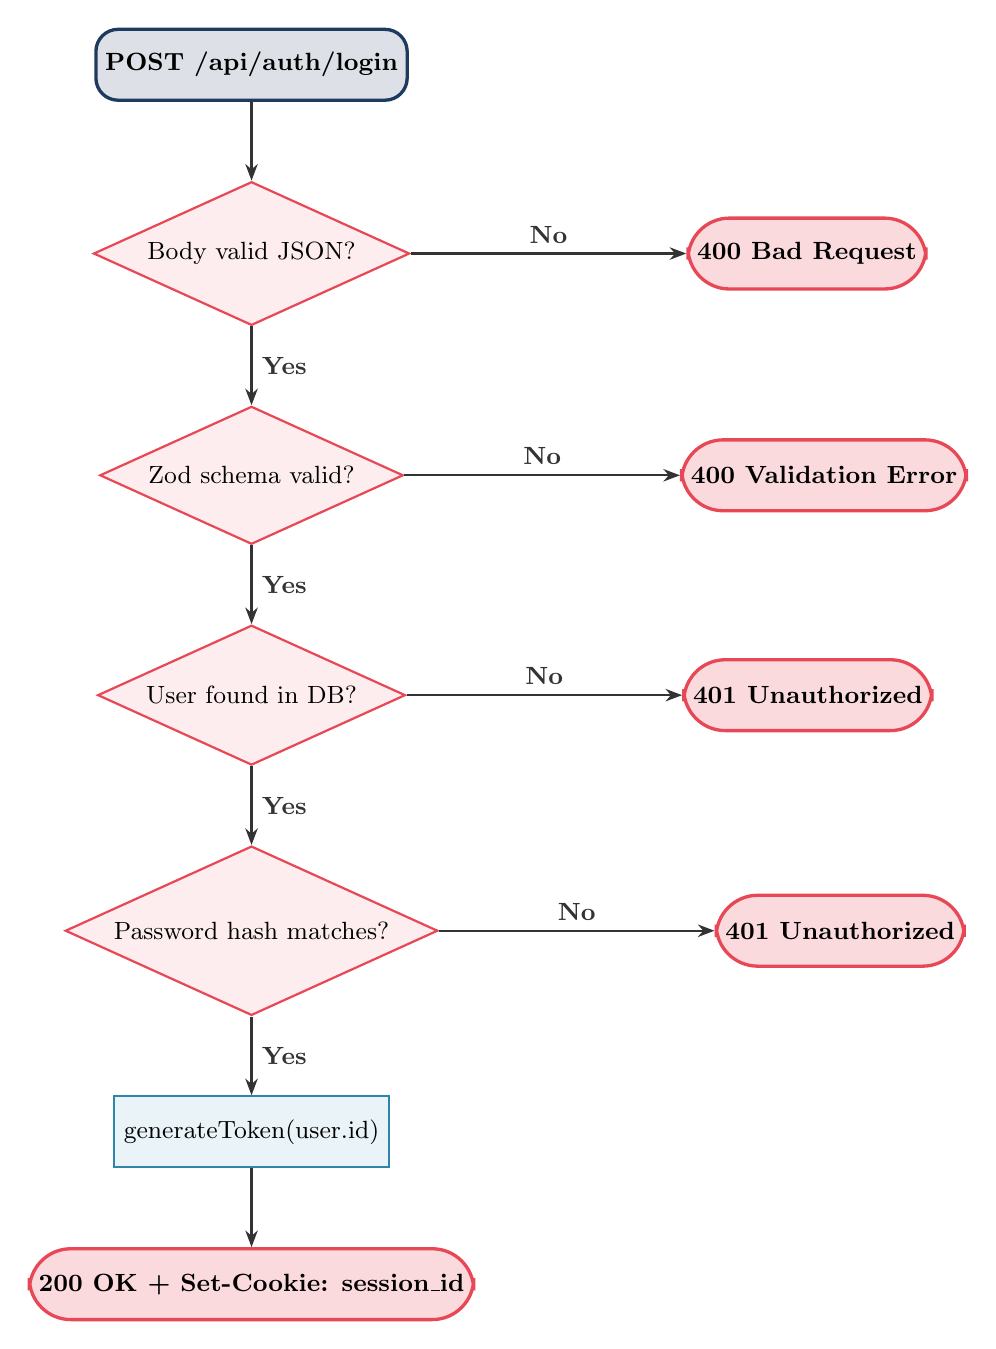
\begin{tikzpicture}[node distance=1.0cm]
  \node[startstop] (start) {POST /api/auth/login};
  \node[decision,below=of start] (d1) {Body valid JSON?};
  \node[terminal,right=3.5cm of d1] (r400a) {400 Bad Request};
  \node[decision,below=of d1] (d2) {Zod schema valid?};
  \node[terminal,right=3.5cm of d2] (r400b) {400 Validation Error};
  \node[decision,below=of d2] (d3) {User found in DB?};
  \node[terminal,right=3.5cm of d3] (r401a) {401 Unauthorized};
  \node[decision,below=of d3] (d4) {Password hash matches?};
  \node[terminal,right=3.5cm of d4] (r401b) {401 Unauthorized};
  \node[process,below=of d4] (token) {generateToken(user.id)};
  \node[terminal,below=of token] (r200) {200 OK + Set-Cookie: session\_id};
  \draw[arrow] (start)--(d1);
  \draw[arrow] (d1)--node[no,above]{No}(r400a);
  \draw[arrow] (d1)--node[yes,right]{Yes}(d2);
  \draw[arrow] (d2)--node[no,above]{No}(r400b);
  \draw[arrow] (d2)--node[yes,right]{Yes}(d3);
  \draw[arrow] (d3)--node[no,above]{No}(r401a);
  \draw[arrow] (d3)--node[yes,right]{Yes}(d4);
  \draw[arrow] (d4)--node[no,above]{No}(r401b);
  \draw[arrow] (d4)--node[yes,right]{Yes}(token);
  \draw[arrow] (token)--(r200);
\end{tikzpicture}
\caption{Login API authentication flow}
\end{figure}

\subsection{API Endpoint Reference}

\begin{center}
\begin{longtable}{llp{6cm}}
  \toprule
  \textbf{Method + Path} & \textbf{Auth} & \textbf{Description} \\
  \midrule
  \endhead
  POST /api/auth/register    & Public  & Register new user \\
  POST /api/auth/login       & Public  & Login, set session cookie \\
  POST /api/auth/logout      & Auth    & Clear session cookie \\
  GET  /api/auth/session     & Auth    & Get current session user \\
  GET|POST /api/products     & Auth    & List / create products \\
  GET|PATCH|DELETE /api/products/[id] & Auth & Get / update / delete product \\
  GET /api/products/import   & Admin   & Bulk import from CSV/Excel \\
  GET|POST /api/orders       & Auth    & List / create orders \\
  GET|PATCH|DELETE /api/orders/[id] & Auth & Get / update / delete order \\
  GET|POST /api/invoices     & Auth    & List / create invoices \\
  GET /api/invoices/[id]/pdf & Auth    & Generate invoice PDF \\
  POST /api/invoices/[id]/send & Auth  & Send invoice email \\
  POST /api/payments/checkout & Auth   & Create Stripe Checkout session \\
  POST /api/payments/webhook & Public  & Stripe webhook handler \\
  GET /api/dashboard         & Admin   & Admin dashboard stats \\
  GET /api/portal/client     & Client  & Client dashboard \\
  GET /api/portal/supplier   & Supplier & Supplier dashboard \\
  GET /api/forecasting       & Admin   & Demand forecasting data \\
  GET /api/ai/insights       & Admin   & AI business insights \\
  GET|POST /api/support-tickets & Auth & List / create tickets \\
  GET|POST /api/users        & Admin   & List / create users \\
  GET /api/audit-logs        & Admin   & Audit log entries \\
  GET|PATCH /api/system-config & Admin & System configuration \\
  GET /api/health            & Public  & Health check \\
  GET /api/openapi           & Public  & OpenAPI specification \\
  \bottomrule
\end{longtable}
\end{center}

\section{Frontend Architecture}

\subsection{Component Hierarchy}

The frontend follows a layered component architecture:

\begin{itemize}[leftmargin=1.5em]
  \item \textbf{Layout Components:} \texttt{Navbar}, \texttt{AdminSidebar}, \texttt{PageWithSidebar} --- provide the structural shell for each role's experience.
  \item \textbf{Page Components:} Located in \texttt{components/Pages/} --- orchestrate data fetching and compose domain components.
  \item \textbf{Domain Components:} Located in \texttt{components/[domain]/} --- e.g., \texttt{ProductList}, \texttt{OrderDialog}, \texttt{InvoiceTable} --- handle domain-specific UI and interactions.
  \item \textbf{UI Primitives:} Located in \texttt{components/ui/} --- shadcn/ui components (Button, Dialog, Table, Badge, etc.) built on Radix UI for accessibility.
  \item \textbf{Shared Components:} \texttt{ErrorBoundary}, \texttt{PaginationSelector}, \texttt{LoadingSpinner} --- reused across domains.
\end{itemize}

\subsection{State Management}

\begin{center}
\begin{tabularx}{\textwidth}{lX}
  \toprule
  \textbf{State Type} & \textbf{Solution} \\
  \midrule
  Server state (API data) & TanStack Query (React Query) --- handles caching, background refetch, optimistic updates \\
  Client UI state         & Zustand stores --- lightweight, no boilerplate, used for modals, filters, selections \\
  Form state              & React Hook Form --- uncontrolled inputs, Zod resolver for validation \\
  Auth state              & React Context (\texttt{AuthContext}) --- provides current user to all components \\
  Theme state             & \texttt{ThemeProvider} with \texttt{localStorage} persistence \\
  \bottomrule
\end{tabularx}
\end{center}

\subsection{Data Fetching Pattern}

All data fetching uses TanStack Query hooks defined in \texttt{hooks/queries/}. Each hook wraps an Axios call to the corresponding API endpoint:

\begin{lstlisting}[language=JavaScript,caption={Example TanStack Query hook for products}]
// hooks/queries/useProducts.ts
export const useProducts = (filters: ProductFilters) => {
  return useQuery({
    queryKey: ['products', filters],
    queryFn: () => apiClient.get('/api/products', { params: filters }),
    staleTime: 30_000, // 30 seconds
  });
};
\end{lstlisting}

Cache invalidation is handled centrally via \texttt{lib/react-query/invalidate-all.ts}, which provides typed invalidation helpers for each resource type.

% ═════════════════════════════════════════════════════════════════════════════

\chapter{System Diagrams}
\section{UML Class Diagram}
The UML class diagram provides an overview of the system's core entities and their relationships.
\begin{figure}[h!]
    \centering
    \includegraphics[width=\textwidth]{"Uml_daigram.png"}
    \caption{System UML Class Diagram}
\end{figure}

\section{Entity Relationship Diagram (ERD)}
The ER diagram illustrates the database schema layout and table constraints.
\begin{figure}[h!]
    \centering
    \includegraphics[width=\textwidth]{"erdplus.png"}
    \caption{Entity Relationship Diagram}
\end{figure}

\section{Data Flow Architecture}
The DFA shows how data correctly travels through inputs, processing logic, and outputs.
\begin{figure}[h!]
    \centering
    \includegraphics[width=\textwidth]{"Data Flow Architecture.png"}
    \caption{Data Flow Architecture Diagram}
\end{figure}

\section{Activity Diagram}
The Activity diagram highlights the workflows of users through the different portals.
\begin{figure}[h!]
    \centering
    \includegraphics[width=0.8\textwidth]{"activity_daigram.png"}
    \caption{System Activity Diagram}
\end{figure}

\section{Non-Functional Requirements and Stereotypes}
The following diagram showcases various NFR characteristics mapped across the modules.
\begin{figure}[h!]
    \centering
    \includegraphics[width=0.9\textwidth]{"NFR and Stereotypes.jpeg"}
    \caption{NFR and Stereotypes Diagram}
\end{figure}

\chapter{Implementation Details}
% ═════════════════════════════════════════════════════════════════════════════

\section{Authentication System}

\subsection{JWT Token Management}

The authentication system is implemented in \texttt{utils/auth.ts} (server-side) and \texttt{utils/auth.client.ts} (client-side). The server-side module uses the \texttt{jsonwebtoken} library with dynamic import to prevent bundling on the client.

\begin{lstlisting}[language=JavaScript,caption={Token generation and verification (utils/auth.ts)}]
// Token generation
export const generateToken = (userId: string): string => {
  return jwt.sign({ userId }, JWT_SECRET, { expiresIn: "1h" });
};

// Token verification with 5 distinct branches
export const verifyToken = (token: string): { userId: string } | null => {
  // Branch A: falsy, "null", or "undefined" string
  if (!token || token === "null" || token === "undefined") return null;
  // Branch B: client-side execution guard
  if (typeof window !== "undefined") return null;
  // Branch C: jwt module unavailable
  const jwt = require("jsonwebtoken");
  if (!jwt?.verify) return null;
  try {
    // Branch E: successful verification
    const decoded = jwt.verify(token, JWT_SECRET) as { userId: string };
    return { userId: decoded.userId };
  } catch {
    // Branch D: expired, invalid, or malformed token
    return null;
  }
};
\end{lstlisting}

The client-side module (\texttt{utils/auth.client.ts}) avoids direct JWT operations entirely, instead making an API call to \texttt{/api/auth/session} with \texttt{credentials: "include"} to let the server verify the \texttt{httpOnly} cookie:

\begin{lstlisting}[language=JavaScript,caption={Client-side session retrieval}]
export const getSessionClient = async (): Promise<User | null> => {
  try {
    const response = await fetch("/api/auth/session", {
      method: "GET",
      credentials: "include", // sends httpOnly session_id cookie
    });
    return response.ok ? await response.json() : null;
  } catch {
    return null;
  }
};
\end{lstlisting}

\subsection{Password Security}

Passwords are hashed using bcrypt with 10 salt rounds before storage. The \texttt{hashPassword} and \texttt{comparePassword} functions provide a clean abstraction:

\begin{lstlisting}[language=JavaScript,caption={Password hashing and comparison}]
export const hashPassword = async (password: string): Promise<string> => {
  const salt = await bcrypt.genSalt(10);
  return bcrypt.hash(password, salt);
};

export const comparePassword = async (
  password: string,
  hashedPassword: string
): Promise<boolean> => {
  return bcrypt.compare(password, hashedPassword);
};
\end{lstlisting}

\section{Order Management and Stock Reservation}

\subsection{Stock Reservation State Machine}

The order management system implements a critical stock reservation pattern to prevent overselling. The available stock formula is:
\[
\text{availableStock} = \text{quantity} - \text{reservedQuantity}
\]

\begin{tcolorbox}[criticalbox,title={Critical Stock Reservation Logic}]
\begin{itemize}[leftmargin=1.5em]
  \item \textbf{Order CREATE (pending):} \texttt{reservedQuantity} \textbf{INCREASES} --- stock is reserved but not yet deducted.
  \item \textbf{Order CONFIRM / PAY:} \texttt{quantity} \textbf{DECREASES}, \texttt{reservedQuantity} \textbf{DECREASES} --- stock is physically consumed.
  \item \textbf{Order CANCEL (was pending):} \texttt{reservedQuantity} \textbf{DECREASES} --- reservation is released.
  \item \textbf{Order CANCEL (was confirmed/paid):} \texttt{quantity} \textbf{INCREASES} --- stock is restored.
\end{itemize}
\end{tcolorbox}

\begin{figure}[h!]
\centering
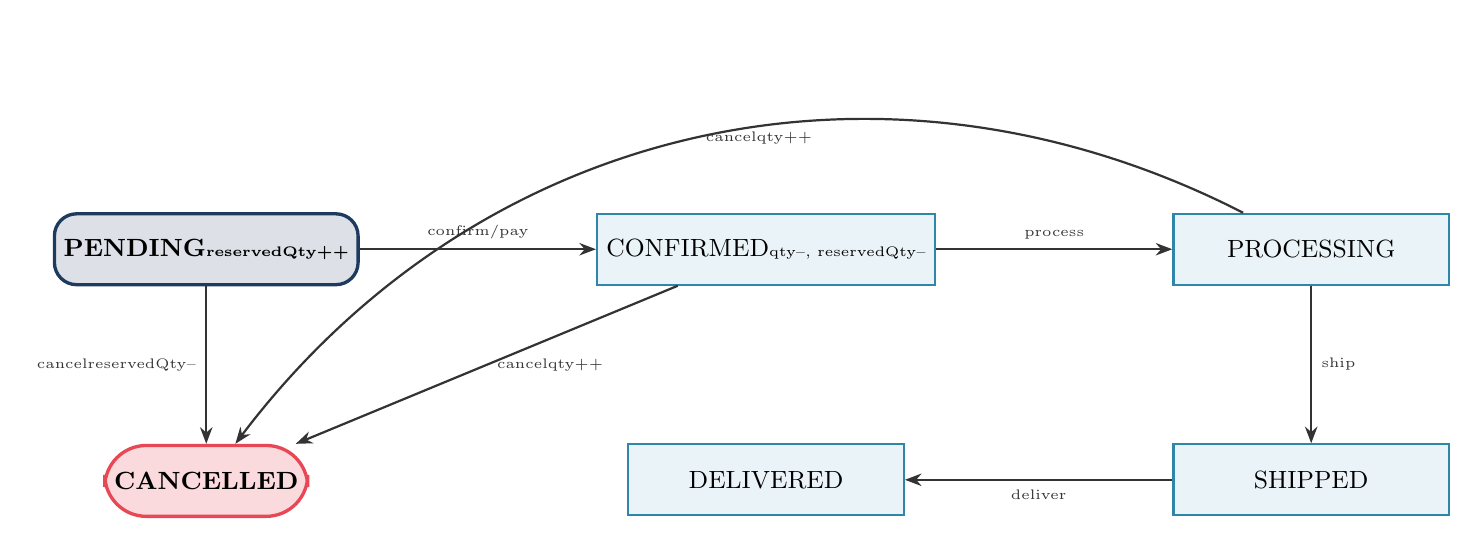
\begin{tikzpicture}[node distance=1.8cm,every node/.style={font=\small}]
  \node[startstop] (pending) {PENDING\\{\tiny reservedQty++}};
  \node[process,right=3cm of pending] (confirmed) {CONFIRMED\\{\tiny qty--, reservedQty--}};
  \node[process,right=3cm of confirmed] (processing) {PROCESSING};
  \node[process,below=2cm of processing] (shipped) {SHIPPED};
  \node[process,below=2cm of confirmed] (delivered) {DELIVERED};
  \node[terminal,below=2cm of pending] (cancelled) {CANCELLED};
  \draw[arrow] (pending)--node[above]{\tiny confirm/pay}(confirmed);
  \draw[arrow] (confirmed)--node[above]{\tiny process}(processing);
  \draw[arrow] (processing)--node[right]{\tiny ship}(shipped);
  \draw[arrow] (shipped)--node[below]{\tiny deliver}(delivered);
  \draw[arrow] (pending)--node[left]{\tiny cancel\\{\tiny reservedQty--}}(cancelled);
  \draw[arrow] (confirmed)--node[right]{\tiny cancel\\{\tiny qty++}}(cancelled);
  \draw[arrow] (processing) to[bend right=40] node[right]{\tiny cancel\\{\tiny qty++}}(cancelled);
\end{tikzpicture}
\caption{Order status state machine with stock side-effects}
\end{figure}

\subsection{Order Creation Algorithm}

\begin{lstlisting}[language=JavaScript,caption={createOrder core logic (prisma/order.ts)}]
async function createOrder(data, userId) {
  const orderNumber = await generateOrderNumber();
  const orderItemsData = [];
  const productsToReserve = [];

  // Validate all items BEFORE any DB writes (fail-fast)
  for (const item of data.items) {
    const product = await prisma.product.findUnique({
      where: { id: item.productId }
    });
    if (!product) throw new Error(`Product not found: ${item.productId}`);

    const availableStock = product.quantity - (product.reservedQuantity ?? 0);
    if (availableStock < item.quantity) {
      throw new Error(
        `Insufficient stock for ${product.name}. ` +
        `Available: ${availableStock}, Requested: ${item.quantity}`
      );
    }
    orderItemsData.push({ ...item, price: product.price });
    productsToReserve.push({ id: product.id, qty: item.quantity });
  }

  // Create order (single DB write)
  const order = await prisma.order.create({ data: { orderNumber, ...data } });

  // Reserve stock for each product
  for (const { id, qty } of productsToReserve) {
    await prisma.product.update({
      where: { id },
      data: { reservedQuantity: { increment: qty } }
    });
  }
  return order;
}
\end{lstlisting}

\section{Invoice Generation and Financial Logic}

\subsection{Invoice Number Generation}

Invoice numbers use a random 4-digit suffix with a uniqueness check loop:

\begin{lstlisting}[language=JavaScript,caption={generateInvoiceNumber with collision handling}]
async function generateInvoiceNumber(): Promise<string> {
  let invoiceNumber: string;
  let exists: boolean;
  do {
    const datePart = format(new Date(), "yyyyMMdd");
    const timePart = format(new Date(), "HHmmss");
    const randomPart = Math.floor(1000 + Math.random() * 9000);
    invoiceNumber = `INV-${datePart}-${timePart}-${randomPart}`;
    exists = !!(await prisma.invoice.findUnique({ where: { invoiceNumber } }));
  } while (exists);
  return invoiceNumber;
}
\end{lstlisting}

\subsection{Financial Calculation Logic}

\begin{lstlisting}[language=JavaScript,caption={Invoice total calculation with safety guards}]
// Nullish coalescing respects explicit 0 values from request
const tax      = data.tax      ?? order.tax      ?? 0;
const shipping = data.shipping ?? order.shipping ?? 0;
const discount = data.discount ?? order.discount ?? 0;

// Math.max(0, ...) prevents negative totals
const total = Math.max(0, subtotal + tax + shipping - discount);

// Invoice always starts unpaid
const amountPaid = 0;
const amountDue  = total;
\end{lstlisting}

The use of \texttt{??} (nullish coalescing) instead of \texttt{||} (logical OR) is critical: it ensures that an explicit \texttt{data.tax = 0} is respected and not overridden by \texttt{order.tax = 15}. With \texttt{||}, zero would be treated as falsy and the fallback would incorrectly apply.

\section{Demand Forecasting Engine}

The forecasting engine (\texttt{lib/forecasting/demand-forecast.ts}) implements several statistical algorithms:

\subsection{Moving Average Calculation}

\begin{lstlisting}[language=JavaScript,caption={Weighted moving average with partial window support}]
function calculateMovingAverage(values: number[], window: number): number[] {
  return values.map((_, i) => {
    const start = Math.max(0, i - window + 1); // partial window for early indices
    const windowValues = values.slice(start, i + 1);
    return windowValues.reduce((a, b) => a + b, 0) / windowValues.length;
  });
}
\end{lstlisting}

\subsection{Standard Deviation (Population)}

\begin{lstlisting}[language=JavaScript,caption={Population standard deviation}]
function calculateStdDev(values: number[]): number {
  if (values.length === 0) return 0; // early return for empty array
  const mean = values.reduce((a, b) => a + b, 0) / values.length;
  const squaredDiffs = values.map(v => Math.pow(v - mean, 2));
  const avgSquaredDiff = squaredDiffs.reduce((a, b) => a + b, 0) / values.length;
  return Math.sqrt(avgSquaredDiff); // population std dev (divides by N, not N-1)
}
\end{lstlisting}

\subsection{Predicted Daily Sales Formula}

When at least 7 days of recent data are available, the system uses a weighted blend:
\[
\text{predictedDailySales} = 0.7 \times \text{recentAvg} + 0.3 \times \text{historicalAvg}
\]
This gives more weight to recent trends while anchoring to historical patterns.

\subsection{Confidence Score Algorithm}

\begin{lstlisting}[language=JavaScript,caption={Confidence score computation}]
let confidence = 50; // base score
if (dailySales.length >= 30) confidence += 30;
else if (dailySales.length >= 14) confidence += 20;
else if (dailySales.length >= 7)  confidence += 10;

const cv = stdDev / averageDailySales; // coefficient of variation
if (cv < 0.3) confidence += 20; // low variability = high confidence
else if (cv < 0.5) confidence += 10;

confidence = Math.min(100, confidence); // cap at 100
\end{lstlisting}

\section{Rate Limiting and Caching}

\subsection{Rate Limiting}

Rate limiting is implemented via Upstash Redis using a sliding window algorithm. The \texttt{withRateLimit} middleware wraps API handlers:

\begin{lstlisting}[language=JavaScript,caption={Rate limiting middleware pattern}]
// lib/api/rate-limit.ts
export async function withRateLimit(
  request: NextRequest,
  handler: () => Promise<NextResponse>
): Promise<NextResponse> {
  const ip = request.ip ?? "anonymous";
  const { success, limit, remaining, reset } = await ratelimit.limit(ip);
  if (!success) {
    return NextResponse.json(
      { error: "Too many requests" },
      { status: 429, headers: { "Retry-After": String(reset) } }
    );
  }
  return handler();
}
\end{lstlisting}

\subsection{Redis Caching}

The caching layer (\texttt{lib/cache/}) provides \texttt{getCache} and \texttt{setCache} utilities with configurable TTLs. Cache keys follow a namespaced pattern (e.g., \texttt{products:list:page1}, \texttt{dashboard:admin:userId}). Cache invalidation is triggered after any write operation via fire-and-forget calls.

\section{Input Validation with Zod}

All API inputs are validated using Zod schemas defined in \texttt{lib/validations/}. Each schema provides:
\begin{itemize}[leftmargin=1.5em]
  \item Type coercion (e.g., string to number for query params)
  \item Field-level error messages
  \item Optional field handling with defaults
  \item Enum validation for status fields
\end{itemize}

\begin{lstlisting}[language=JavaScript,caption={Example Zod schema for order creation}]
export const createOrderSchema = z.object({
  clientId: z.string().optional(),
  items: z.array(z.object({
    productId: z.string().min(1, "Product ID required"),
    quantity: z.number().int().positive("Quantity must be positive"),
  })).min(1, "At least one item required"),
  tax:      z.number().min(0).optional(),
  shipping: z.number().min(0).optional(),
  discount: z.number().min(0).optional(),
  notes:    z.string().optional(),
});
\end{lstlisting}

\section{Stripe Payment Integration}

The Stripe integration handles two flows:

\begin{enumerate}[leftmargin=1.5em]
  \item \textbf{Checkout Session Creation:} \texttt{POST /api/payments/checkout} creates a Stripe Checkout session with line items derived from the invoice. The client is redirected to Stripe's hosted payment page.
  \item \textbf{Webhook Processing:} \texttt{POST /api/payments/webhook} receives Stripe events. The \texttt{checkout.session.completed} event triggers invoice status update to \texttt{paid} and order payment status update to \texttt{paid}. Webhook signature verification using \texttt{STRIPE\_WEBHOOK\_SECRET} prevents spoofed events.
\end{enumerate}

\section{Email Notification System}

Email notifications are sent via Brevo (Sendinblue) with optional QStash queuing for background processing. The notification system supports:
\begin{itemize}[leftmargin=1.5em]
  \item Invoice email delivery with PDF attachment
  \item Overdue invoice reminders (scheduled via \texttt{INTERNAL\_API\_KEY}-protected endpoint)
  \item Low-stock alerts
  \item Order status update notifications
\end{itemize}

Users can configure their email preferences per notification type via \texttt{GET|PUT /api/user/email-preferences}, stored as a JSON field on the \texttt{User} model.

% ═════════════════════════════════════════════════════════════════════════════

\chapter{Detailed Implementation Walkthrough}
\section{Authentication System Deep Dive}

\subsection{JWT Token Lifecycle}

The JWT token lifecycle in Stockly follows a strict server-side-only pattern. The \texttt{jsonwebtoken} library is dynamically imported using \texttt{require()} inside the \texttt{verifyToken} function rather than a top-level \texttt{import}. This is a deliberate architectural decision to prevent the library from being bundled into client-side JavaScript, which would expose the JWT implementation details and potentially the secret to the browser.

The token payload contains only the \texttt{userId} field --- a minimal payload that reduces token size and avoids storing sensitive user data in the token itself. On each authenticated request, the server extracts the \texttt{userId} from the token and performs a fresh database lookup to get the current user state. This means that role changes, account deactivation, or other user updates take effect immediately on the next request, without requiring token invalidation.

\begin{lstlisting}[language=JavaScript,caption={Complete verifyToken implementation}]
export const verifyToken = (token: string): { userId: string } | null => {
  // Branch A: Guard against falsy, "null", or "undefined" string tokens
  // These can occur when cookies are serialized as strings
  if (!token || token === "null" || token === "undefined") {
    return null;
  }

  // Branch B: Prevent execution on client side
  // The jwt library should never run in the browser
  if (typeof window !== "undefined") {
    return null;
  }

  // Branch C: Dynamic import guard
  // jwt may be undefined in edge runtime environments
  const jwt = require("jsonwebtoken");
  if (!jwt || typeof jwt.verify !== "function") {
    return null;
  }

  const JWT_SECRET = process.env.JWT_SECRET || "your_jwt_secret";
  // WARNING: Default secret is a security risk in production!

  try {
    // Branch E: Successful verification
    const decoded = jwt.verify(token, JWT_SECRET) as { userId: string };
    return { userId: decoded.userId };
  } catch (error) {
    // Branch D: Token expired, invalid signature, or malformed
    // All JWT errors are caught here and return null
    return null;
  }
};
\end{lstlisting}

\subsection{Session Resolution Flow}

The \texttt{getSessionFromRequest} function is the primary entry point for all authenticated API routes. It performs a two-step verification: first validating the JWT token, then confirming the user still exists in the database. This two-step approach ensures that deleted or deactivated users cannot continue to use valid tokens.

\begin{lstlisting}[language=JavaScript,caption={getSessionFromRequest implementation}]
export const getSessionFromRequest = async (
  request: NextRequest
): Promise<User | null> => {
  // Step 1: Extract the session_id cookie
  const cookie = request.cookies.get("session_id");
  if (!cookie?.value) return null;

  // Step 2: Verify the JWT token
  const decoded = verifyToken(cookie.value);
  if (!decoded) return null;

  // Step 3: Confirm user exists in database
  // This handles the case where a user was deleted after token issuance
  const user = await prisma.user.findUnique({
    where: { id: decoded.userId },
    select: {
      id: true, name: true, email: true, role: true,
      username: true, image: true, emailPreferences: true,
      // NOTE: password is explicitly excluded from the select
    },
  });

  return user; // null if user not found
};
\end{lstlisting}

\subsection{Google OAuth Flow}

The Google OAuth integration follows the standard OAuth 2.0 authorization code flow:

\begin{enumerate}[leftmargin=1.5em]
  \item User clicks ``Sign in with Google'' button.
  \item Frontend redirects to \texttt{GET /api/auth/oauth/google} which generates the Google authorization URL with the required scopes (\texttt{openid}, \texttt{email}, \texttt{profile}).
  \item User authenticates with Google and grants permissions.
  \item Google redirects to \texttt{GET /api/auth/oauth/google/callback} with an authorization code.
  \item Server exchanges the code for an access token and fetches the user's Google profile.
  \item If a user with the Google ID exists, they are logged in. If not, a new account is created with the Google profile data.
  \item A JWT session cookie is set and the user is redirected to the appropriate dashboard.
\end{enumerate}

\section{Order Management Deep Dive}

\subsection{Order Number Generation Algorithm}

The order number format \texttt{ORD-YYYY-MMDD-HHMMSS-NNNN} is designed to be:
\begin{itemize}[leftmargin=1.5em]
  \item \textbf{Human-readable:} The date and time components make it easy to identify when an order was placed.
  \item \textbf{Sortable:} Lexicographic sorting of order numbers produces chronological order.
  \item \textbf{Unique (with caveats):} The sequence number is based on the count of orders created today, which is not atomic under high concurrency.
\end{itemize}

\begin{lstlisting}[language=JavaScript,caption={generateOrderNumber implementation}]
export const generateOrderNumber = async (): Promise<string> => {
  const now = new Date();
  const year = now.getFullYear();
  const month = String(now.getMonth() + 1).padStart(2, "0");
  const day = String(now.getDate()).padStart(2, "0");
  const hours = String(now.getHours()).padStart(2, "0");
  const minutes = String(now.getMinutes()).padStart(2, "0");
  const seconds = String(now.getSeconds()).padStart(2, "0");

  // Count orders created today for the sequence number
  const todayStart = new Date(year, now.getMonth(), now.getDate());
  const todayEnd = new Date(year, now.getMonth(), now.getDate() + 1);

  const todayOrders = await prisma.order.count({
    where: { createdAt: { gte: todayStart, lt: todayEnd } },
  });

  // Sequence is count + 1, padded to 4 digits
  // NOTE: This is NOT atomic - race condition possible under high concurrency
  const sequence = String(todayOrders + 1).padStart(4, "0");

  return `ORD-${year}-${month}${day}-${hours}${minutes}${seconds}-${sequence}`;
};
\end{lstlisting}

\subsection{Multi-Item Order Validation Strategy}

The order creation algorithm uses a \textbf{fail-fast validation} strategy: all items are validated before any database writes occur. This ensures that if any item fails validation (product not found, insufficient stock), the entire order is rejected without any partial state being written to the database.

This is critical for data integrity. Without fail-fast validation, a scenario like this could occur:
\begin{enumerate}[leftmargin=1.5em]
  \item Item 1 (Widget A, qty 5): Valid, stock reserved.
  \item Item 2 (Widget B, qty 999): Invalid, insufficient stock.
  \item Error thrown --- but Widget A's reservation was already written!
\end{enumerate}

With fail-fast validation, the loop validates ALL items first, collecting them into \texttt{orderItemsData} and \texttt{productsToReserve} arrays. Only after all items pass validation does the code proceed to create the order and reserve stock.

\subsection{Stock Reservation Consistency}

The stock reservation system maintains the invariant:
\[
\text{availableStock} = \text{quantity} - \text{reservedQuantity} \geq 0
\]

This invariant is maintained through careful state machine transitions:

\begin{center}
\begin{tabularx}{\textwidth}{lXX}
  \toprule
  \textbf{Event} & \textbf{quantity change} & \textbf{reservedQuantity change} \\
  \midrule
  Order created (pending)    & 0 (no change)    & +qty (reserve) \\
  Order confirmed/paid       & -qty (deduct)    & -qty (release reservation) \\
  Order cancelled (pending)  & 0 (no change)    & -qty (release reservation) \\
  Order cancelled (confirmed+) & +qty (restore) & 0 (already released) \\
  \bottomrule
\end{tabularx}
\end{center}

The net effect of a complete order lifecycle (create $\to$ confirm $\to$ deliver) is:
\begin{itemize}[leftmargin=1.5em]
  \item \texttt{quantity} decreases by the ordered quantity (stock consumed).
  \item \texttt{reservedQuantity} returns to its original value (reservation created then released).
\end{itemize}

The net effect of a cancelled order (create $\to$ cancel from pending) is:
\begin{itemize}[leftmargin=1.5em]
  \item \texttt{quantity} unchanged (no stock consumed).
  \item \texttt{reservedQuantity} returns to its original value (reservation created then released).
\end{itemize}

\section{Invoice Financial Logic Deep Dive}

\subsection{The Nullish Coalescing Pattern}

The invoice creation logic uses nullish coalescing (\texttt{??}) rather than logical OR (\texttt{||}) for a critical reason. Consider the following scenario:

\begin{itemize}[leftmargin=1.5em]
  \item An order has \texttt{tax = 15.00} (15\% tax applied at order time).
  \item When creating the invoice, the admin explicitly sets \texttt{data.tax = 0} (tax-exempt invoice).
\end{itemize}

With \texttt{||}: \texttt{data.tax || order.tax || 0 = 0 || 15 || 0 = 15} (WRONG --- zero is falsy!)

With \texttt{??}: \texttt{data.tax ?? order.tax ?? 0 = 0 ?? 15 ?? 0 = 0} (CORRECT --- zero is not null/undefined!)

This distinction is critical for financial accuracy. The \texttt{??} operator only falls back to the right operand when the left operand is \texttt{null} or \texttt{undefined}, not when it is \texttt{0}, \texttt{false}, or \texttt{""}.

\subsection{Negative Total Prevention}

The \texttt{Math.max(0, ...)} guard prevents negative invoice totals in scenarios where discounts exceed the sum of subtotal, tax, and shipping. While a negative total might seem like an edge case, it can occur legitimately when:
\begin{itemize}[leftmargin=1.5em]
  \item A large promotional discount is applied.
  \item A correction invoice is created for an overpayment.
  \item Data entry errors result in an oversized discount.
\end{itemize}

Rather than throwing an error, the system clamps the total to zero, which is the correct financial behavior (the customer owes nothing, but does not receive a refund through this mechanism).

\subsection{Invoice Status State Machine}

\begin{figure}[h!]
\centering
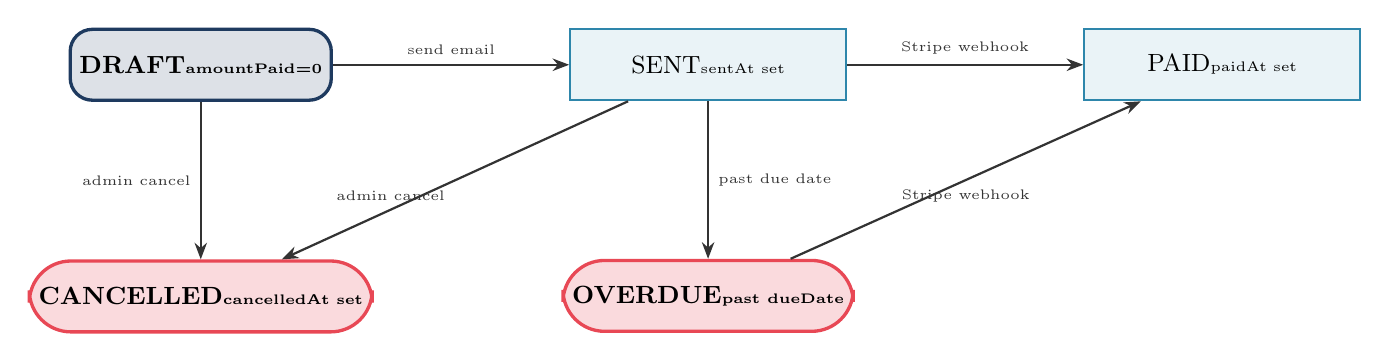
\begin{tikzpicture}[node distance=2cm,every node/.style={font=\small}]
  \node[startstop] (draft) {DRAFT\\{\tiny amountPaid=0}};
  \node[process,right=3cm of draft] (sent) {SENT\\{\tiny sentAt set}};
  \node[process,right=3cm of sent] (paid) {PAID\\{\tiny paidAt set}};
  \node[terminal,below=2cm of sent] (overdue) {OVERDUE\\{\tiny past dueDate}};
  \node[terminal,below=2cm of draft] (cancelled) {CANCELLED\\{\tiny cancelledAt set}};
  \draw[arrow] (draft)--node[above]{\tiny send email}(sent);
  \draw[arrow] (sent)--node[above]{\tiny Stripe webhook}(paid);
  \draw[arrow] (sent)--node[right]{\tiny past due date}(overdue);
  \draw[arrow] (draft)--node[left]{\tiny admin cancel}(cancelled);
  \draw[arrow] (sent)--node[below left]{\tiny admin cancel}(cancelled);
  \draw[arrow] (overdue)--node[below]{\tiny Stripe webhook}(paid);
\end{tikzpicture}
\caption{Invoice status state machine}
\end{figure}

\section{Demand Forecasting Deep Dive}

\subsection{Linear Regression for Trend Analysis}

The \texttt{analyzeTrend} function uses simple linear regression to determine the sales trend direction. Given $n$ data points $(x_i, y_i)$ where $x_i$ is the day index and $y_i$ is the daily sales quantity, the slope is computed as:

\[
\text{slope} = \frac{n \sum x_i y_i - \sum x_i \sum y_i}{n \sum x_i^2 - (\sum x_i)^2}
\]

The percentage change is then computed as:
\[
\text{percentageChange} = \frac{\text{slope} \times n \times 100}{\bar{y}}
\]

where $\bar{y}$ is the mean daily sales. This normalizes the slope by the average sales volume, making the percentage change comparable across products with different sales volumes.

\subsection{Z-Score Anomaly Detection}

The anomaly detection algorithm uses z-scores to identify days with unusually high or low sales:

\[
z_i = \frac{|y_i - \bar{y}|}{\sigma}
\]

where $\bar{y}$ is the mean and $\sigma$ is the population standard deviation. Days with $z_i > 2.0$ (the \texttt{ANOMALY\_THRESHOLD}) are flagged as anomalies. The severity classification is:

\begin{center}
\begin{tabular}{cll}
  \toprule
  \textbf{Z-Score Range} & \textbf{Severity} & \textbf{Interpretation} \\
  \midrule
  $z > 3.0$   & High   & Extreme outlier (3+ standard deviations) \\
  $2.5 < z \leq 3.0$ & Medium & Significant outlier \\
  $2.0 < z \leq 2.5$ & Low    & Mild outlier \\
  $z \leq 2.0$ & None  & Normal variation \\
  \bottomrule
\end{tabular}
\end{center}

The anomaly type (spike vs drop) is determined by comparing the day's sales to the mean:
\begin{itemize}[leftmargin=1.5em]
  \item \texttt{spike}: $y_i > \bar{y}$ (unusually high sales)
  \item \texttt{drop}: $y_i < \bar{y}$ (unusually low sales)
\end{itemize}

\subsection{Weighted Prediction Formula}

When at least 7 days of recent data are available, the predicted daily sales uses a weighted blend that gives more importance to recent trends:

\[
\text{predicted} = 0.7 \times \text{recentAvg} + 0.3 \times \text{historicalAvg}
\]

The 70/30 weighting was chosen empirically to balance responsiveness to recent trends with stability from historical data. A higher weight on recent data (e.g., 90/10) would make the forecast more volatile; a lower weight (e.g., 50/50) would make it slower to respond to genuine trend changes.

\section{API Security Architecture}

\subsection{Defense in Depth}

Stockly implements multiple layers of security:

\begin{enumerate}[leftmargin=1.5em]
  \item \textbf{Transport Security:} All production traffic uses HTTPS (enforced by Vercel). The \texttt{session\_id} cookie has the \texttt{Secure} flag set in production.
  \item \textbf{Authentication:} JWT tokens with 1-hour expiry. The \texttt{httpOnly} cookie flag prevents JavaScript access, mitigating XSS attacks.
  \item \textbf{Authorization:} Role-based access control enforced at the API route level. Every protected route calls \texttt{getSessionFromRequest} and checks the user's role.
  \item \textbf{Input Validation:} All API inputs are validated with Zod schemas before processing. Invalid inputs return structured 400 errors.
  \item \textbf{Rate Limiting:} Upstash Redis-based rate limiting prevents brute-force attacks and API abuse.
  \item \textbf{CORS:} Cross-Origin Resource Sharing headers are configured to allow only trusted origins.
  \item \textbf{Webhook Verification:} Stripe webhook signatures are verified using \texttt{stripe.webhooks.constructEvent} to prevent spoofed payment events.
  \item \textbf{Audit Logging:} All create, update, and delete operations are recorded in the \texttt{AuditLog} collection with user ID, action, entity type, and timestamp.
\end{enumerate}

\subsection{CORS Configuration}

\begin{lstlisting}[language=JavaScript,caption={CORS configuration in lib/api/cors.ts}]
export const corsHeaders = {
  "Access-Control-Allow-Origin": process.env.NEXT_PUBLIC_APP_URL || "*",
  "Access-Control-Allow-Methods": "GET, POST, PATCH, DELETE, OPTIONS",
  "Access-Control-Allow-Headers": "Content-Type, Authorization",
  "Access-Control-Allow-Credentials": "true",
};

export function handleCors(request: NextRequest): NextResponse | null {
  if (request.method === "OPTIONS") {
    return new NextResponse(null, { status: 200, headers: corsHeaders });
  }
  return null;
}
\end{lstlisting}

\section{Caching Strategy}

\subsection{Cache Key Design}

Cache keys follow a hierarchical naming convention to enable targeted invalidation:

\begin{center}
\begin{tabularx}{\textwidth}{lX}
  \toprule
  \textbf{Cache Key Pattern} & \textbf{Description} \\
  \midrule
  \texttt{products:list:\{page\}:\{filters\}} & Paginated product list with filters \\
  \texttt{products:detail:\{id\}} & Single product detail \\
  \texttt{orders:list:\{userId\}:\{page\}} & User-scoped order list \\
  \texttt{orders:detail:\{id\}} & Single order detail \\
  \texttt{invoices:list:\{userId\}:\{page\}} & User-scoped invoice list \\
  \texttt{dashboard:admin:\{userId\}} & Admin dashboard stats \\
  \texttt{dashboard:client:\{userId\}} & Client dashboard stats \\
  \texttt{dashboard:supplier:\{supplierId\}} & Supplier dashboard stats \\
  \texttt{forecasting:\{productId\}} & Product demand forecast \\
  \bottomrule
\end{tabularx}
\end{center}

\subsection{Cache TTL Strategy}

\begin{center}
\begin{tabularx}{\textwidth}{lXl}
  \toprule
  \textbf{Resource} & \textbf{Rationale} & \textbf{TTL} \\
  \midrule
  Product list      & Changes frequently (stock updates) & 30 seconds \\
  Product detail    & Changes on stock updates & 30 seconds \\
  Order list        & Changes on new orders & 60 seconds \\
  Dashboard stats   & Aggregated, acceptable staleness & 5 minutes \\
  Forecasting data  & Computationally expensive, slow-changing & 1 hour \\
  Categories        & Rarely changes & 10 minutes \\
  Suppliers         & Rarely changes & 10 minutes \\
  \bottomrule
\end{tabularx}
\end{center}

\section{Email System Architecture}

\subsection{Email Queue with QStash}

For high-volume email scenarios (e.g., sending invoices to many clients), the system uses QStash (Upstash's message queue) to process emails asynchronously:

\begin{enumerate}[leftmargin=1.5em]
  \item API route receives the email request and enqueues a job to QStash.
  \item QStash delivers the job to the \texttt{/api/email/queue} endpoint.
  \item The endpoint verifies the QStash signature and processes the email.
  \item If the email fails, QStash automatically retries with exponential backoff.
\end{enumerate}

This pattern prevents email failures from blocking the API response and provides automatic retry logic for transient failures.

\subsection{Email Template System}

Email templates are defined in \texttt{lib/email/templates/} as TypeScript functions that return HTML strings. Each template accepts typed parameters and produces responsive HTML email content compatible with major email clients.

\begin{lstlisting}[language=JavaScript,caption={Invoice email template structure}]
export const invoiceEmailTemplate = (params: {
  clientName: string;
  invoiceNumber: string;
  total: number;
  dueDate: Date;
  paymentLink?: string;
}): { subject: string; html: string } => ({
  subject: `Invoice ${params.invoiceNumber} - Payment Due`,
  html: `
    <div style="font-family: Arial, sans-serif; max-width: 600px;">
      <h1>Invoice ${params.invoiceNumber}</h1>
      <p>Dear ${params.clientName},</p>
      <p>Your invoice for <strong>$${params.total.toFixed(2)}</strong> 
         is due on ${params.dueDate.toLocaleDateString()}.</p>
      ${params.paymentLink ? 
        `<a href="${params.paymentLink}">Pay Now</a>` : ''}
    </div>
  `,
});
\end{lstlisting}

\section{Notification System}

\subsection{In-App Notification Types}

The notification system supports the following notification types, each with a corresponding icon and color in the UI:

\begin{center}
\begin{tabularx}{\textwidth}{llX}
  \toprule
  \textbf{Type} & \textbf{Trigger} & \textbf{Description} \\
  \midrule
  \texttt{low\_stock}           & Product quantity falls below threshold & Alert admin/supplier to reorder \\
  \texttt{stock\_out}           & Product quantity reaches 0 & Critical alert for out-of-stock \\
  \texttt{order\_confirmation}  & New order created & Notify admin of new order \\
  \texttt{order\_status\_update} & Order status changes & Notify client of status change \\
  \texttt{invoice\_sent}        & Invoice emailed to client & Confirm invoice delivery \\
  \texttt{payment\_received}    & Stripe webhook confirms payment & Notify admin of payment \\
  \texttt{support\_ticket}      & New support ticket created & Notify assigned admin \\
  \texttt{review\_submitted}    & New product review submitted & Notify admin for moderation \\
  \bottomrule
\end{tabularx}
\end{center}

\subsection{Notification API}

\begin{center}
\begin{tabularx}{\textwidth}{llX}
  \toprule
  \textbf{Endpoint} & \textbf{Method} & \textbf{Description} \\
  \midrule
  \texttt{/api/notifications/in-app}              & GET   & List notifications for current user \\
  \texttt{/api/notifications/in-app}              & PATCH & Mark notifications as read \\
  \texttt{/api/notifications/in-app/unread-count} & GET   & Get unread notification count \\
  \texttt{/api/notifications/in-app/[id]}         & PATCH & Mark single notification as read \\
  \texttt{/api/notifications/in-app/[id]}         & DELETE & Delete a notification \\
  \bottomrule
\end{tabularx}
\end{center}

\section{Product Import System}

\subsection{CSV/Excel Import Flow}

The bulk product import system (\texttt{GET /api/products/import}) supports both CSV and Excel (.xlsx) file formats. The import process follows these steps:

\begin{enumerate}[leftmargin=1.5em]
  \item \textbf{File Upload:} Client uploads the file via multipart form data.
  \item \textbf{Format Detection:} File extension determines the parser (CSV or Excel).
  \item \textbf{Row Parsing:} Each row is parsed into a product object.
  \item \textbf{Row Validation:} Each row is validated against the product Zod schema.
  \item \textbf{Batch Insert:} Valid rows are inserted in batches to avoid timeout.
  \item \textbf{Error Collection:} Invalid rows are collected with row numbers and error messages.
  \item \textbf{History Recording:} An \texttt{ImportHistory} record is created with success/failure counts.
  \item \textbf{Response:} Returns summary with \texttt{successRows}, \texttt{failedRows}, and \texttt{errors} array.
\end{enumerate}

\subsection{Import Validation Rules}

\begin{center}
\begin{tabularx}{\textwidth}{llX}
  \toprule
  \textbf{Field} & \textbf{Required} & \textbf{Validation} \\
  \midrule
  name       & Yes & Non-empty string \\
  sku        & Yes & Non-empty string, must be unique \\
  price      & Yes & Positive number \\
  quantity   & Yes & Non-negative integer \\
  categoryId & Yes & Valid MongoDB ObjectId, must exist \\
  supplierId & Yes & Valid MongoDB ObjectId, must exist \\
  status     & No  & One of: available, stock\_low, out\_of\_stock (default: available) \\
  description & No & String \\
  expirationDate & No & Valid ISO date string \\
  \bottomrule
\end{tabularx}
\end{center}

\section{Audit Logging System}

\subsection{Audit Log Schema}

Every significant action in the system is recorded in the \texttt{AuditLog} collection:

\begin{lstlisting}[language=JavaScript,caption={AuditLog model}]
model AuditLog {
  id         String   @id @default(auto()) @map("_id") @db.ObjectId
  userId     String   @db.ObjectId  // Who performed the action
  action     String   // create | update | delete | login | logout | import
  entityType String   // product | order | invoice | user | category | supplier
  entityId   String?  @db.ObjectId  // ID of the affected entity
  details    Json?    // Before/after values for updates
  ipAddress  String?  // Client IP address
  userAgent  String?  // Browser/client user agent
  createdAt  DateTime @default(now()) @db.Date

  @@index([userId])
  @@index([action])
  @@index([entityType])
  @@index([createdAt])
}
\end{lstlisting}

\subsection{Audit Log Usage}

The audit log is used for:
\begin{itemize}[leftmargin=1.5em]
  \item \textbf{Compliance:} Providing a complete trail of all data changes for regulatory requirements.
  \item \textbf{Debugging:} Tracing the sequence of events that led to a data inconsistency.
  \item \textbf{Security:} Detecting unauthorized access patterns or suspicious activity.
  \item \textbf{Activity History:} Powering the admin's ``Activity History'' and ``My Activity'' pages.
\end{itemize}

The admin can view audit logs via \texttt{GET /api/audit-logs} with filtering by user, action type, entity type, and date range.

\section{System Configuration}

\subsection{SystemConfig Model}

The \texttt{SystemConfig} model provides a flexible key-value store for admin-managed application settings:

\begin{center}
\begin{tabularx}{\textwidth}{llX}
  \toprule
  \textbf{Key} & \textbf{Type} & \textbf{Description} \\
  \midrule
  \texttt{company\_name}        & string  & Company name displayed in emails and PDFs \\
  \texttt{low\_stock\_threshold} & number  & Quantity below which products are marked ``stock\_low'' \\
  \texttt{invoice\_due\_days}   & number  & Default days until invoice due date \\
  \texttt{tax\_rate}            & number  & Default tax rate percentage \\
  \texttt{currency}             & string  & Default currency code (e.g., USD, EUR) \\
  \texttt{timezone}             & string  & System timezone for date calculations \\
  \texttt{email\_notifications} & boolean & Global toggle for email notifications \\
  \bottomrule
\end{tabularx}
\end{center}

Settings are cached in Redis with a 10-minute TTL to avoid repeated database queries on every request.



% ─── Packages ────────────────────────────────────────────────────────────────
\usepackage[a4paper, margin=2.5cm]{geometry}
\usepackage[T1]{fontenc}
\usepackage[utf8]{inputenc}
\usepackage{lmodern}
\usepackage{microtype}
\usepackage{xcolor}
\usepackage{graphicx}
\usepackage{booktabs}
\usepackage{longtable}
\usepackage{array}
\usepackage{tabularx}
\usepackage{multirow}
\usepackage{enumitem}
\usepackage{listings}
\usepackage{fancyhdr}
\usepackage{titlesec}
\usepackage{tocloft}
\usepackage{hyperref}
\usepackage{amsmath}
\usepackage{amssymb}
\usepackage{tikz}
\usetikzlibrary{shapes.geometric,arrows.meta,positioning,fit,backgrounds,calc}
\usepackage{tcolorbox}
\tcbuselibrary{skins,breakable}
\usepackage{setspace}
\usepackage{caption}
\usepackage{subcaption}
\usepackage{mdframed}

% ─── Colour Palette ──────────────────────────────────────────────────────────
\definecolor{primary}{HTML}{1E3A5F}
\definecolor{secondary}{HTML}{2E86AB}
\definecolor{accent}{HTML}{E84855}
\definecolor{success}{HTML}{3BB273}
\definecolor{warning}{HTML}{F4A261}
\definecolor{lightgray}{HTML}{F5F5F5}
\definecolor{darkgray}{HTML}{333333}
\definecolor{codebg}{HTML}{1E1E2E}
\definecolor{codetext}{HTML}{CDD6F4}
\definecolor{p1red}{HTML}{C0392B}
\definecolor{p2orange}{HTML}{E67E22}
\definecolor{p3blue}{HTML}{2980B9}
\definecolor{p4green}{HTML}{27AE60}
\definecolor{titlebg}{HTML}{0D1B2A}

% ─── Hyperref ────────────────────────────────────────────────────────────────
\hypersetup{
  colorlinks=true, linkcolor=primary, urlcolor=secondary, citecolor=accent,
  pdftitle={Stockly -- Comprehensive Project Report},
  pdfauthor={Stockly Engineering Team},
  pdfsubject={Software Engineering Project Report},
}

% ─── Header / Footer ─────────────────────────────────────────────────────────
\pagestyle{fancy}
\fancyhf{}
\fancyhead[L]{\small\color{primary}\textbf{Stockly} --- Inventory \& Supply Chain Management}
\fancyhead[R]{\small\color{darkgray}v2.0.1 $\cdot$ April 2026}
\fancyfoot[C]{\small\color{darkgray}\thepage}
\renewcommand{\headrulewidth}{0.4pt}
\renewcommand{\footrulewidth}{0.4pt}

% ─── Section Styling ─────────────────────────────────────────────────────────
\titleformat{\chapter}[display]
  {\normalfont\huge\bfseries\color{primary}}{\chaptertitlename\ \thechapter}{20pt}{\Huge}
\titleformat{\section}{\normalfont\Large\bfseries\color{primary}}{\thesection}{1em}{}
\titleformat{\subsection}{\normalfont\large\bfseries\color{secondary}}{\thesubsection}{1em}{}
\titleformat{\subsubsection}{\normalfont\normalsize\bfseries\color{darkgray}}{\thesubsubsection}{1em}{}

% ─── Code Style ──────────────────────────────────────────────────────────────
\lstdefinestyle{codestyle}{
  backgroundcolor=\color{codebg}, basicstyle=\ttfamily\footnotesize\color{codetext},
  keywordstyle=\color{accent}\bfseries, commentstyle=\color{success}\itshape,
  stringstyle=\color{warning}, breaklines=true, frame=single,
  rulecolor=\color{secondary}, numbers=left, numberstyle=\tiny\color{darkgray},
  tabsize=2, showstringspaces=false,
}
\lstset{style=codestyle}

% ─── Custom Boxes ────────────────────────────────────────────────────────────
\tcbset{
  reqbox/.style={enhanced,breakable,colback=blue!4,colframe=primary,
    fonttitle=\bfseries\color{white},coltitle=white,
    attach boxed title to top left,
    boxed title style={colback=primary,rounded corners},rounded corners},
  testbox/.style={enhanced,breakable,colback=lightgray,colframe=secondary,
    fonttitle=\bfseries\color{white},coltitle=white,
    attach boxed title to top left,
    boxed title style={colback=secondary,rounded corners},
    rounded corners,drop shadow},
  criticalbox/.style={enhanced,breakable,colback=red!5,colframe=p1red,
    fonttitle=\bfseries\color{white},coltitle=white,
    attach boxed title to top left,
    boxed title style={colback=p1red,rounded corners},rounded corners},
  infobox/.style={enhanced,breakable,colback=blue!5,colframe=primary,
    fonttitle=\bfseries\color{white},coltitle=white,
    attach boxed title to top left,
    boxed title style={colback=primary,rounded corners},rounded corners},
  warningbox/.style={enhanced,breakable,colback=orange!8,colframe=warning,
    fonttitle=\bfseries\color{white},coltitle=white,
    attach boxed title to top left,
    boxed title style={colback=warning,rounded corners},rounded corners},
  successbox/.style={enhanced,breakable,colback=green!5,colframe=success,
    fonttitle=\bfseries\color{white},coltitle=white,
    attach boxed title to top left,
    boxed title style={colback=success,rounded corners},rounded corners},
}

% ─── TikZ Styles ─────────────────────────────────────────────────────────────
\tikzset{
  startstop/.style={rectangle,rounded corners=8pt,minimum width=3cm,
    minimum height=0.9cm,text centered,draw=primary,very thick,
    fill=primary!15,font=\small\bfseries},
  process/.style={rectangle,minimum width=3.5cm,minimum height=0.9cm,
    text centered,draw=secondary,thick,fill=secondary!10,font=\small},
  decision/.style={diamond,aspect=2.2,minimum width=3.5cm,minimum height=0.9cm,
    text centered,draw=accent,thick,fill=accent!10,font=\small},
  terminal/.style={rectangle,rounded corners=15pt,minimum width=2.5cm,
    minimum height=0.9cm,text centered,draw=accent,very thick,
    fill=accent!20,font=\small\bfseries},
  arrow/.style={-{Stealth[length=6pt]},thick,color=darkgray},
  yes/.style={font=\small\color{success}\bfseries},
  no/.style={font=\small\color{accent}\bfseries},
}

% ─── Helpers ─────────────────────────────────────────────────────────────────
\newcommand{\pone}{\textbf{\color{p1red}P1}}
\newcommand{\ptwo}{\textbf{\color{p2orange}P2}}
\newcommand{\pthree}{\textbf{\color{p3blue}P3}}
\newcommand{\pfour}{\textbf{\color{p4green}P4}}
\newcommand{\req}[1]{\texttt{\textbf{\color{primary}#1}}}
\newcommand{\api}[1]{\texttt{\color{secondary}#1}}
\newcommand{\model}[1]{\texttt{\color{accent}#1}}

\setlength{\parskip}{7pt}
\setlength{\parindent}{0pt}
\onehalfspacing

% ═════════════════════════════════════════════════════════════════════════════

% ═════════════════════════════════════════════════════════════════════════════

% ─── TITLE PAGE ──────────────────────────────────────────────────────────────
\begin{titlepage}
  \pagecolor{titlebg}\color{white}\centering
  \vspace*{1.2cm}
  {\fontsize{11}{14}\selectfont\texttt{\color{secondary}SOFTWARE ENGINEERING PROJECT REPORT}}\\[0.4cm]
  \rule{14cm}{0.5pt}\\[0.9cm]
  {\fontsize{44}{54}\selectfont\bfseries\color{white}Stockly}\\[0.3cm]
  {\fontsize{17}{22}\selectfont\color{secondary}Inventory \& Supply Chain Management System}\\[0.7cm]
  \rule{14cm}{0.5pt}\\[0.9cm]
  {\large\itshape\color{white!85}
    A Full-Stack Role-Based Warehouse, Order, Invoice, and Analytics Platform\\[0.2cm]
    Built with Next.js~16, TypeScript~5, Prisma~ORM~6.4, and MongoDB
  }\\[2.2cm]
  \begin{tabular}{rl}
    \textbf{\color{secondary}Version:}         & \color{white}2.0.1 \\[4pt]
    \textbf{\color{secondary}Date:}            & \color{white}April 8, 2026 \\[4pt]
    \textbf{\color{secondary}Framework:}       & \color{white}Next.js 16 (App Router), React 19 \\[4pt]
    \textbf{\color{secondary}Language:}        & \color{white}TypeScript 5 (strict mode) \\[4pt]
    \textbf{\color{secondary}Database:}        & \color{white}MongoDB via Prisma ORM 6.4 \\[4pt]
    \textbf{\color{secondary}Live Demo:}       & \color{secondary}\url{https://stockly-inventory.vercel.app} \\[4pt]
    \textbf{\color{secondary}License:}         & \color{white}MIT Open Source \\[4pt]
    \textbf{\color{secondary}Report Type:}     & \color{white}SRS + Architecture + White-Box Testing \\[4pt]
    \textbf{\color{secondary}Test Cases:}      & \color{white}107 across 10 modules \\[4pt]
    \textbf{\color{secondary}Coverage Target:} & \color{white}85\% Statements / 90\% Branch \\
  \end{tabular}
  \vfill
  \rule{14cm}{0.5pt}\\[0.4cm]
  {\small\color{white!55}
    This document covers the complete Software Requirements Specification, system design,\\
    implementation details, white-box testing strategy, deployment, and future roadmap.
  }
\end{titlepage}
\pagecolor{white}\color{black}

% ─── ABSTRACT ────────────────────────────────────────────────────────────────
\chapter*{Abstract}
\addcontentsline{toc}{chapter}{Abstract}

\begin{tcolorbox}[infobox,title={Executive Summary}]
Stockly is a production-grade, role-based inventory and supply chain management platform that consolidates product management, order processing, invoice generation, warehouse tracking, supplier coordination, customer support, and business analytics into a single cohesive web application. The system serves three distinct user roles --- administrators, suppliers, and clients --- each with tailored dashboards and access controls enforced at both the API and UI layers.
\end{tcolorbox}

This report presents the complete software engineering documentation for Stockly v2.0.1. It covers the Software Requirements Specification (SRS) with functional and non-functional requirements, system architecture and data model design, implementation details of critical algorithms and integrations, a comprehensive white-box testing strategy with 107 documented test cases across 10 modules, deployment procedures for both local and cloud environments, and a future development roadmap.

The platform is built on a modern full-stack architecture: \textbf{Next.js 16} with the App Router paradigm for server-side rendering and API routes, \textbf{TypeScript 5} in strict mode for end-to-end type safety, \textbf{Prisma ORM 6.4} with \textbf{MongoDB} as the persistence layer, and \textbf{JWT-based authentication} with \textbf{bcryptjs} for secure session management. Optional integrations include Stripe (payments), Shippo (shipping), Brevo (transactional email), ImageKit (media), Upstash Redis (caching and rate limiting), Sentry (error monitoring), and OpenRouter (AI insights).

The core business logic encompasses product lifecycle management with SKU tracking and QR code generation, a multi-state order management system with atomic stock reservation semantics, invoice generation with financial integrity guarantees (including negative-total prevention via \texttt{Math.max(0, ...)}), demand forecasting using statistical moving averages and z-score anomaly detection, and a comprehensive RBAC system. White-box testing targets 85\% statement coverage and 90\% branch coverage across all critical modules, with special emphasis on security-critical paths (JWT verification, password hashing), financial logic (invoice totals, stock reservation), and edge cases (null coalescing, boundary values).

\textbf{Key outcomes:} The system reduces manual inventory tracking overhead, provides real-time stock visibility, automates order-to-invoice workflows, and delivers actionable business intelligence through integrated analytics and AI-assisted forecasting.

\newpage

% ─── TABLE OF CONTENTS ───────────────────────────────────────────────────────
\tableofcontents
\newpage

% ═════════════════════════════════════════════════════════════════════════════

\chapter{Project Management and Development Process}
\section{Development Methodology}

Stockly was developed following an iterative Agile methodology with two-week sprints. The development process was organized into the following phases:

\begin{enumerate}[leftmargin=1.5em]
  \item \textbf{Phase 1 --- Foundation (Weeks 1--2):} Project setup, database schema design, authentication system, basic CRUD for products and categories.
  \item \textbf{Phase 2 --- Core Business Logic (Weeks 3--4):} Order management with stock reservation, invoice generation, warehouse management.
  \item \textbf{Phase 3 --- Role-Based Portals (Weeks 5--6):} Supplier portal, client portal, role-based dashboards, RBAC enforcement.
  \item \textbf{Phase 4 --- Integrations (Weeks 7--8):} Stripe payments, Shippo shipping, Brevo email, ImageKit image upload.
  \item \textbf{Phase 5 --- Analytics and AI (Weeks 9--10):} Business insights charts, demand forecasting engine, AI insights via OpenRouter.
  \item \textbf{Phase 6 --- Support and Reviews (Weeks 11--12):} Support ticket system, product reviews, notification system.
  \item \textbf{Phase 7 --- Testing and Hardening (Weeks 13--14):} White-box testing, security review, performance optimization, documentation.
  \item \textbf{Phase 8 --- Deployment (Week 15):} Production deployment on Vercel, MongoDB Atlas setup, environment configuration.
\end{enumerate}

\section{Version Control Strategy}

The project uses Git with the following branching strategy:

\begin{itemize}[leftmargin=1.5em]
  \item \textbf{main:} Production-ready code. Protected branch requiring pull request review.
  \item \textbf{develop:} Integration branch for completed features.
  \item \textbf{feature/[name]:} Feature branches created from develop.
  \item \textbf{fix/[name]:} Bug fix branches created from main (for hotfixes) or develop.
\end{itemize}

\section{Code Quality Standards}

\subsection{TypeScript Configuration}

The project uses TypeScript in strict mode with the following compiler options:

\begin{lstlisting}[language=JSON,caption={tsconfig.json strict settings}]
{
  "compilerOptions": {
    "strict": true,
    "noUncheckedIndexedAccess": true,
    "noImplicitReturns": true,
    "noFallthroughCasesInSwitch": true,
    "exactOptionalPropertyTypes": true
  }
}
\end{lstlisting}

\subsection{ESLint Configuration}

The project uses ESLint with the Next.js recommended configuration plus additional rules:

\begin{lstlisting}[language=JSON,caption={.eslintrc.json}]
{
  "extends": ["next/core-web-vitals", "next/typescript"],
  "rules": {
    "no-console": ["warn", { "allow": ["warn", "error"] }],
    "@typescript-eslint/no-explicit-any": "error",
    "@typescript-eslint/no-unused-vars": "error"
  }
}
\end{lstlisting}

\section{API Documentation}

\subsection{OpenAPI Specification}

The system exposes an OpenAPI 3.0 specification at \texttt{GET /api/openapi}. This specification is used to:
\begin{itemize}[leftmargin=1.5em]
  \item Power the in-app API documentation page (\texttt{/api-docs}).
  \item Enable client SDK generation for third-party integrations.
  \item Provide a machine-readable contract for API consumers.
\end{itemize}

\subsection{In-App API Documentation}

The \texttt{/api-docs} page renders the OpenAPI specification using a documentation UI, providing:
\begin{itemize}[leftmargin=1.5em]
  \item Interactive endpoint explorer with request/response examples.
  \item Authentication instructions.
  \item Schema definitions for all request and response bodies.
  \item Error code reference.
\end{itemize}

\section{Monitoring and Observability}

\subsection{Sentry Integration}

When \texttt{SENTRY\_DSN} is configured, Sentry captures:
\begin{itemize}[leftmargin=1.5em]
  \item Unhandled exceptions in API routes with full stack traces.
  \item React component rendering errors via Error Boundaries.
  \item Performance traces for slow API routes (configurable threshold).
  \item User context (userId, role) attached to error reports for debugging.
\end{itemize}

\subsection{Health Check Endpoint}

The \texttt{GET /api/health} endpoint provides a comprehensive system status check:

\begin{lstlisting}[language=JavaScript,caption={Health check implementation}]
export async function GET() {
  const checks = {
    database: "unknown",
    redis: "unknown",
    stripe: process.env.STRIPE_API_KEY ? "configured" : "not_configured",
    brevo: process.env.BREVO_API_KEY ? "configured" : "not_configured",
    shippo: process.env.SHIPPO_API_KEY ? "configured" : "not_configured",
  };

  // Check database connectivity
  try {
    await prisma.$queryRaw`{ ping: 1 }`;
    checks.database = "connected";
  } catch {
    checks.database = "error";
  }

  // Check Redis connectivity
  try {
    if (redis) {
      await redis.ping();
      checks.redis = "connected";
    } else {
      checks.redis = "not_configured";
    }
  } catch {
    checks.redis = "error";
  }

  const allHealthy = checks.database === "connected";
  return NextResponse.json(
    { status: allHealthy ? "ok" : "degraded", ...checks },
    { status: allHealthy ? 200 : 503 }
  );
}
\end{lstlisting}

\chapter{Testing and Deployment}
% ═════════════════════════════════════════════════════════════════════════════

\section{White-Box Testing Strategy}

\begin{tcolorbox}[infobox,title={What is White-Box Testing?}]
White-box testing (also called \textbf{structural testing}, \textbf{glass-box testing}, or \textbf{clear-box testing}) examines the \emph{internal} logic, code paths, branches, loops, and data flows of an application --- not just its external behaviour. It requires full knowledge of the source code and targets 100\% statement, branch, and path coverage of critical modules.
\end{tcolorbox}

\subsection{Testing Goals}

\begin{itemize}[leftmargin=1.5em]
  \item Achieve \textbf{85\% statement coverage} across all modules.
  \item Achieve \textbf{90\% branch coverage} --- every \texttt{if}/\texttt{else} branch tested.
  \item Validate all \texttt{catch} blocks are reachable and handled correctly.
  \item Verify all loops execute correctly for 0, 1, and $N$ iterations.
  \item Confirm financial calculations produce mathematically correct results.
  \item Ensure security boundaries (JWT, RBAC) cannot be bypassed.
\end{itemize}

\subsection{Types of White-Box Testing Applied}

\begin{enumerate}[leftmargin=1.5em]
  \item \textbf{Unit Testing} --- Individual functions tested in isolation with mocked dependencies.
  \item \textbf{Integration Testing} --- API route handlers tested end-to-end with mocked Prisma.
  \item \textbf{Control Flow Testing} --- All branches and decision points covered.
  \item \textbf{Data Flow Testing} --- Tracking how data is created, transformed, and consumed.
  \item \textbf{Boundary Value Analysis} --- Testing edge values at limits (e.g., exact stock match, zero discount).
  \item \textbf{Mutation Testing} --- Verifying tests catch intentional code bugs.
\end{enumerate}

\subsection{Priority Classification}

\begin{center}
\begin{tabular}{clp{9cm}}
  \toprule
  \textbf{Priority} & \textbf{Label} & \textbf{Meaning} \\
  \midrule
  \pone & Critical & Security, financial logic, auth guards. Must pass before any release. \\
  \ptwo & High     & Core business logic, stock management, role-based access. \\
  \pthree & Medium & Edge cases, format validation, confidence scores. \\
  \pfour & Low     & Informational, documentation-level tests. \\
  \bottomrule
\end{tabular}
\end{center}

% ─── MODULE 1: AUTH ───────────────────────────────────────────────────────────
\section{Module 1: Authentication \& Session Management}

\textbf{Source Files:} \texttt{utils/auth.ts}, \texttt{utils/auth.client.ts}, \texttt{app/api/auth/login/route.ts}

\subsection{verifyToken Branch Map}

\begin{tcolorbox}[warningbox,title={Security-Critical Function --- 5 Branches}]
\texttt{verifyToken} has 5 distinct branches. All must be covered. The \texttt{JWT\_SECRET} defaults to \texttt{"your\_jwt\_secret"} if the environment variable is not set --- a \textbf{critical security risk} in production.
\end{tcolorbox}

\begin{center}
\begin{tabular}{clp{7cm}}
  \toprule
  \textbf{Branch} & \textbf{Condition} & \textbf{Result} \\
  \midrule
  A & \texttt{token} is falsy, \texttt{"null"}, or \texttt{"undefined"} & \texttt{return null} \\
  B & \texttt{typeof window !== "undefined"} (client-side) & \texttt{return null} \\
  C & \texttt{jwt} module undefined or \texttt{jwt.verify} missing & \texttt{return null} \\
  D & \texttt{jwt.verify} throws (expired / invalid / malformed) & \texttt{catch} $\to$ \texttt{return null} \\
  E & \texttt{jwt.verify} succeeds & \texttt{return \{ userId \}} \\
  \bottomrule
\end{tabular}
\end{center}

\begin{tcolorbox}[testbox,title={AUTH-001 \hfill \pone}]
\textbf{Function:} \texttt{verifyToken} \quad \textbf{Scenario:} Token is an empty string \\
\textbf{Input:} \texttt{token = ""} \\
\textbf{Expected Path:} Branch A (falsy check) $\to$ \texttt{return null} \\
\textbf{Expected Output:} \texttt{null} \quad \textbf{Coverage:} Statement + Branch A
\end{tcolorbox}

\begin{tcolorbox}[testbox,title={AUTH-002 \hfill \pone}]
\textbf{Function:} \texttt{verifyToken} \quad \textbf{Scenario:} Token is the string \texttt{"null"} \\
\textbf{Input:} \texttt{token = "null"} \\
\textbf{Expected Path:} Branch A (string \texttt{"null"} check) $\to$ \texttt{return null} \\
\textbf{Expected Output:} \texttt{null} \quad \textbf{Coverage:} Branch A edge case
\end{tcolorbox}

\begin{tcolorbox}[testbox,title={AUTH-003 \hfill \pone}]
\textbf{Function:} \texttt{verifyToken} \quad \textbf{Scenario:} Token is the string \texttt{"undefined"} \\
\textbf{Input:} \texttt{token = "undefined"} \\
\textbf{Expected Path:} Branch A $\to$ \texttt{return null} \\
\textbf{Expected Output:} \texttt{null} \quad \textbf{Coverage:} Branch A edge case
\end{tcolorbox}

\begin{tcolorbox}[testbox,title={AUTH-004 \hfill \pone}]
\textbf{Function:} \texttt{verifyToken} \quad \textbf{Scenario:} Valid JWT token on server side \\
\textbf{Input:} Token generated by \texttt{generateToken("user123")} \\
\textbf{Expected Path:} Branch E $\to$ \texttt{return \{ userId: "user123" \}} \\
\textbf{Expected Output:} \texttt{\{ userId: "user123" \}} \quad \textbf{Coverage:} Happy path
\end{tcolorbox}

\begin{tcolorbox}[criticalbox,title={AUTH-005 \hfill \pone\ --- Expired Token}]
\textbf{Function:} \texttt{verifyToken} \quad \textbf{Scenario:} Expired JWT token \\
\textbf{Input:} Token with \texttt{expiresIn: "1ms"}, verified after 10ms delay \\
\textbf{Expected Path:} Branch D $\to$ \texttt{jwt.verify} throws \texttt{TokenExpiredError} $\to$ \texttt{return null} \\
\textbf{Expected Output:} \texttt{null} \quad \textbf{Coverage:} Exception handling branch
\end{tcolorbox}

\begin{tcolorbox}[criticalbox,title={AUTH-006 \hfill \pone\ --- Wrong Secret}]
\textbf{Function:} \texttt{verifyToken} \quad \textbf{Scenario:} Token signed with wrong secret \\
\textbf{Input:} \texttt{jwt.sign(\{ userId: "x" \}, "WRONG\_SECRET")} \\
\textbf{Expected Path:} Branch D $\to$ \texttt{jwt.verify} throws \texttt{JsonWebTokenError} $\to$ \texttt{return null} \\
\textbf{Expected Output:} \texttt{null} \quad \textbf{Coverage:} Security branch
\end{tcolorbox}

\begin{tcolorbox}[testbox,title={AUTH-007 \hfill \pone}]
\textbf{Function:} \texttt{verifyToken} \quad \textbf{Scenario:} Malformed token string \\
\textbf{Input:} \texttt{token = "not.a.jwt.token"} \\
\textbf{Expected Path:} Branch D $\to$ catch $\to$ \texttt{return null} \\
\textbf{Expected Output:} \texttt{null} \quad \textbf{Coverage:} Malformed input
\end{tcolorbox}

\begin{tcolorbox}[testbox,title={AUTH-008 \hfill \pone}]
\textbf{Function:} \texttt{generateToken} \quad \textbf{Scenario:} Valid userId generates decodable token \\
\textbf{Input:} \texttt{userId = "abc123"} \\
\textbf{Expected:} \texttt{jwt.decode(result).userId === "abc123"} \\
\textbf{Coverage:} Token payload integrity
\end{tcolorbox}

\begin{tcolorbox}[testbox,title={AUTH-009 \hfill \pone}]
\textbf{Function:} \texttt{hashPassword + comparePassword} \quad \textbf{Scenario:} Round-trip verification \\
\textbf{Input:} \texttt{password = "SecurePass123!"} \\
\textbf{Steps:} (1) \texttt{hash = await hashPassword(password)} \quad (2) \texttt{result = await comparePassword(password, hash)} \\
\textbf{Expected:} \texttt{result === true} \quad \textbf{Coverage:} Round-trip password verification
\end{tcolorbox}

\begin{tcolorbox}[testbox,title={AUTH-010 \hfill \pone}]
\textbf{Function:} \texttt{comparePassword} \quad \textbf{Scenario:} Wrong password against valid hash \\
\textbf{Input:} \texttt{comparePassword("WrongPass", hashOf("CorrectPass"))} \\
\textbf{Expected:} \texttt{false} \quad \textbf{Coverage:} Negative comparison branch
\end{tcolorbox}

\begin{tcolorbox}[testbox,title={AUTH-011 \hfill \pone}]
\textbf{Route:} \texttt{POST /api/auth/login} \quad \textbf{Scenario:} Missing email field \\
\textbf{Input:} \texttt{\{ password: "test123" \}} \\
\textbf{Expected Path:} \texttt{loginSchema.parse} throws \texttt{ZodError} $\to$ 400 \\
\textbf{Expected Response:} \texttt{\{ error: "..." \}}, status \textbf{400}
\end{tcolorbox}

\begin{tcolorbox}[testbox,title={AUTH-012 \hfill \pone}]
\textbf{Route:} \texttt{POST /api/auth/login} \quad \textbf{Scenario:} User not found \\
\textbf{Input:} \texttt{\{ email: "nonexistent@test.com", password: "pass" \}} \\
\textbf{Mock:} \texttt{prisma.user.findUnique} returns \texttt{null} \\
\textbf{Expected Response:} \texttt{\{ error: "Invalid email or password" \}}, status \textbf{401}
\end{tcolorbox}

\begin{tcolorbox}[criticalbox,title={AUTH-013 \hfill \ptwo\ --- Corrupted Data}]
\textbf{Route:} \texttt{POST /api/auth/login} \quad \textbf{Scenario:} User found but password is null \\
\textbf{Mock:} \texttt{prisma.user.findUnique} returns \texttt{\{ id: "x", password: null \}} \\
\textbf{Expected Path:} \texttt{!user.password} $\to$ 500 \\
\textbf{Expected Response:} \texttt{\{ error: "User data corrupted: password missing" \}}, status \textbf{500}
\end{tcolorbox}

\begin{tcolorbox}[testbox,title={AUTH-014 \hfill \pone}]
\textbf{Route:} \texttt{POST /api/auth/login} \quad \textbf{Scenario:} Correct credentials --- full happy path \\
\textbf{Input:} \texttt{\{ email: "admin@test.com", password: "correct" \}} \\
\textbf{Mock:} User found, \texttt{bcrypt.compare} returns \texttt{true} \\
\textbf{Expected Response:} Status \textbf{200}, \texttt{Set-Cookie} header with \texttt{session\_id}
\end{tcolorbox}

\begin{tcolorbox}[testbox,title={AUTH-015 \hfill \pone}]
\textbf{Function:} \texttt{getSessionFromRequest} \quad \textbf{Scenario:} No session\_id cookie \\
\textbf{Input:} Request with no cookies \\
\textbf{Expected Path:} \texttt{cookie === undefined} $\to$ \texttt{return null} \\
\textbf{Expected Output:} \texttt{null} \quad \textbf{Coverage:} Missing cookie branch
\end{tcolorbox}

\begin{tcolorbox}[testbox,title={AUTH-016 \hfill \ptwo}]
\textbf{Function:} \texttt{getSessionFromRequest} \quad \textbf{Scenario:} Valid cookie but user deleted from DB \\
\textbf{Mock:} \texttt{prisma.user.findUnique} returns \texttt{null} \\
\textbf{Expected Path:} Decoded OK $\to$ DB query $\to$ \texttt{null} \\
\textbf{Expected Output:} \texttt{null} \quad \textbf{Coverage:} Deleted user edge case
\end{tcolorbox}

% ─── MODULE 2: ORDERS ────────────────────────────────────────────────────────
\section{Module 2: Order Management \& Stock State Machine}

\textbf{Source Files:} \texttt{prisma/order.ts}, \texttt{app/api/orders/route.ts}, \texttt{app/api/orders/[id]/route.ts}

\begin{tcolorbox}[testbox,title={ORD-001 \hfill \ptwo}]
\textbf{Function:} \texttt{generateOrderNumber} \quad \textbf{Scenario:} First order of the day \\
\textbf{Mock:} \texttt{prisma.order.count} returns \texttt{0} \\
\textbf{Expected:} Sequence = \texttt{"0001"}, format: \texttt{ORD-2026-0401-HHMMSS-0001} \\
\textbf{Coverage:} Sequence generation, zero-count branch
\end{tcolorbox}

\begin{tcolorbox}[testbox,title={ORD-002 \hfill \pthree\ --- Boundary}]
\textbf{Function:} \texttt{generateOrderNumber} \quad \textbf{Scenario:} 9999 orders already exist today \\
\textbf{Mock:} \texttt{prisma.order.count} returns \texttt{9999} \\
\textbf{Expected:} Sequence = \texttt{"10000"} (5 digits, overflow of 4-digit pad) \\
\textbf{Note:} Race condition possible under high concurrency --- not atomic \\
\textbf{Coverage:} Boundary value, sequence overflow
\end{tcolorbox}

\begin{tcolorbox}[testbox,title={ORD-003 \hfill \ptwo}]
\textbf{Function:} \texttt{createOrder} \quad \textbf{Scenario:} Product not found \\
\textbf{Input:} \texttt{data.items = [\{ productId: "nonexistent", quantity: 1 \}]} \\
\textbf{Mock:} \texttt{prisma.product.findUnique} returns \texttt{null} \\
\textbf{Expected:} \texttt{throw Error("Product not found: nonexistent")} \\
\textbf{Coverage:} Product not found branch
\end{tcolorbox}

\begin{tcolorbox}[criticalbox,title={ORD-004 \hfill \ptwo\ --- Insufficient Stock}]
\textbf{Function:} \texttt{createOrder} \quad \textbf{Scenario:} Insufficient available stock \\
\textbf{Input:} \texttt{item.quantity = 10} \\
\textbf{Mock:} \texttt{product.quantity = 15}, \texttt{product.reservedQuantity = 8} \\
\textbf{Internal:} \texttt{availableStock = 15 - 8 = 7 < 10} \\
\textbf{Expected:} \texttt{throw Error("Insufficient stock. Available: 7, Requested: 10")} \\
\textbf{Coverage:} Stock check branch (insufficient)
\end{tcolorbox}

\begin{tcolorbox}[testbox,title={ORD-005 \hfill \pthree\ --- Boundary}]
\textbf{Function:} \texttt{createOrder} \quad \textbf{Scenario:} Exactly enough stock \\
\textbf{Input:} \texttt{item.quantity = 7} \\
\textbf{Mock:} \texttt{product.quantity = 15}, \texttt{product.reservedQuantity = 8} \\
\textbf{Internal:} \texttt{availableStock = 7 == 7} (exactly enough) \\
\textbf{Expected:} Order created successfully, no error \\
\textbf{Coverage:} Boundary value (exact stock match)
\end{tcolorbox}

\begin{tcolorbox}[testbox,title={ORD-006 \hfill \pthree\ --- Boundary+1}]
\textbf{Function:} \texttt{createOrder} \quad \textbf{Scenario:} One more than available stock \\
\textbf{Input:} \texttt{item.quantity = 8} \\
\textbf{Mock:} \texttt{product.quantity = 15}, \texttt{product.reservedQuantity = 8} \\
\textbf{Internal:} \texttt{availableStock = 7 < 8} \\
\textbf{Expected:} \texttt{throw Error("Insufficient stock")} \\
\textbf{Coverage:} Boundary value + 1
\end{tcolorbox}

\begin{tcolorbox}[testbox,title={ORD-007 \hfill \pthree}]
\textbf{Function:} \texttt{createOrder} \quad \textbf{Scenario:} reservedQuantity is null \\
\textbf{Mock:} \texttt{product.quantity = 10}, \texttt{product.reservedQuantity = null} \\
\textbf{Internal:} \texttt{availableStock = 10 - Number(null) = 10 - 0 = 10} \\
\textbf{Expected:} availableStock correctly computed as 10 \\
\textbf{Coverage:} Null coalescing in stock calculation
\end{tcolorbox}

\begin{tcolorbox}[criticalbox,title={ORD-008 \hfill \ptwo\ --- Atomicity}]
\textbf{Function:} \texttt{createOrder} \quad \textbf{Scenario:} Multiple items, one fails stock check \\
\textbf{Input:} \texttt{items = [\{ productA, qty: 1 \}, \{ productB, qty: 999 \}]} \\
\textbf{Mock:} productA has stock, productB has only 5 \\
\textbf{Expected:} Error thrown on productB; NO reservation made for productA \\
\textbf{Coverage:} Partial failure rollback (fail-fast before any DB writes)
\end{tcolorbox}

\begin{tcolorbox}[testbox,title={ORD-009 \hfill \ptwo}]
\textbf{Function:} \texttt{createOrder} \quad \textbf{Scenario:} Tax, shipping, discount all provided \\
\textbf{Input:} \texttt{subtotal=100, tax=10, shipping=5, discount=15} \\
\textbf{Expected:} \texttt{total = 100 + 10 + 5 - 15 = 100} \\
\textbf{Coverage:} Total calculation formula
\end{tcolorbox}

\begin{tcolorbox}[testbox,title={ORD-010 \hfill \pthree}]
\textbf{Function:} \texttt{createOrder} \quad \textbf{Scenario:} Tax and shipping are 0 (falsy) \\
\textbf{Input:} \texttt{tax=0, shipping=0, discount=0} \\
\textbf{Internal:} \texttt{tax > 0} is false $\to$ stored as null \\
\textbf{Expected:} \texttt{order.tax = null, order.shipping = null, order.discount = null} \\
\textbf{Coverage:} Falsy-to-null conversion branches
\end{tcolorbox}

\begin{tcolorbox}[testbox,title={ORD-011 \hfill \ptwo}]
\textbf{Function:} \texttt{createOrder} \quad \textbf{Scenario:} Verify reservedQuantity incremented \\
\textbf{Input:} Single item, quantity = 3 \\
\textbf{Mock:} \texttt{product.reservedQuantity = 5} before order \\
\textbf{Expected:} After \texttt{createOrder}, \texttt{product.reservedQuantity = 8} \\
\textbf{Coverage:} Stock reservation side effect
\end{tcolorbox}

\begin{tcolorbox}[testbox,title={ORD-012 \hfill \pone}]
\textbf{Route:} \texttt{GET /api/orders} \quad \textbf{Scenario:} Unauthenticated request \\
\textbf{Mock:} \texttt{getSessionFromRequest} returns \texttt{null} \\
\textbf{Expected:} \texttt{\{ error: "Unauthorized" \}}, status \textbf{401} \\
\textbf{Coverage:} Auth guard branch
\end{tcolorbox}

\begin{tcolorbox}[testbox,title={ORD-013 \hfill \ptwo}]
\textbf{Route:} \texttt{GET /api/orders} \quad \textbf{Scenario:} Supplier with no supplier record \\
\textbf{Mock:} \texttt{session.role = "supplier"}, \texttt{getSupplierByUserId} returns \texttt{null} \\
\textbf{Expected:} \texttt{NextResponse.json([])} --- empty array, not error \\
\textbf{Coverage:} Supplier without record branch
\end{tcolorbox}

\begin{tcolorbox}[testbox,title={ORD-014 \hfill \ptwo}]
\textbf{Route:} \texttt{GET /api/orders} \quad \textbf{Scenario:} Cache hit \\
\textbf{Mock:} \texttt{getCache} returns cached array \\
\textbf{Expected:} Returns cached data without DB query \\
\textbf{Coverage:} Cache hit branch
\end{tcolorbox}

\begin{tcolorbox}[testbox,title={ORD-015 \hfill \ptwo}]
\textbf{Route:} \texttt{GET /api/orders} \quad \textbf{Scenario:} Client role fetches only their orders \\
\textbf{Mock:} \texttt{session.role = "client"}, \texttt{session.id = "clientUserId"} \\
\textbf{Expected:} \texttt{getOrdersByClientId} called with \texttt{"clientUserId"} \\
\textbf{Coverage:} Role-based query branching (client)
\end{tcolorbox}

\begin{tcolorbox}[testbox,title={ORD-016 \hfill \ptwo}]
\textbf{Route:} \texttt{GET /api/orders} \quad \textbf{Scenario:} Rate limit exceeded \\
\textbf{Mock:} \texttt{withRateLimit} returns a 429 response \\
\textbf{Expected:} 429 response returned immediately, no DB query \\
\textbf{Coverage:} Rate limit early return branch
\end{tcolorbox}
% ─── MODULE 3: INVOICES ──────────────────────────────────────────────────────
\section{Module 3: Invoice Generation \& Financial Logic}

\textbf{Source Files:} \texttt{prisma/invoice.ts}, \texttt{app/api/invoices/route.ts}

\begin{tcolorbox}[testbox,title={INV-001 \hfill \ptwo}]
\textbf{Function:} \texttt{generateInvoiceNumber} \quad \textbf{Scenario:} No collision on first attempt \\
\textbf{Mock:} \texttt{prisma.invoice.findUnique} returns \texttt{null} on first call \\
\textbf{Expected:} Returns \texttt{"INV-YYYYMMDD-HHMMSS-XXXX"} format; while loop executes once \\
\textbf{Coverage:} Happy path, no collision
\end{tcolorbox}

\begin{tcolorbox}[testbox,title={INV-002 \hfill \pthree}]
\textbf{Function:} \texttt{generateInvoiceNumber} \quad \textbf{Scenario:} First attempt collides, second unique \\
\textbf{Mock:} \texttt{prisma.invoice.findUnique} returns existing invoice on call 1, \texttt{null} on call 2 \\
\textbf{Expected:} While loop executes twice, returns second generated number \\
\textbf{Coverage:} Collision handling branch (while loop iteration)
\end{tcolorbox}

\begin{tcolorbox}[testbox,title={INV-003 \hfill \pthree}]
\textbf{Function:} \texttt{generateInvoiceNumber} \quad \textbf{Scenario:} Verify format structure \\
\textbf{Expected:} Result matches regex \texttt{/\^{}INV-\textbackslash{}d\{8\}-\textbackslash{}d\{6\}-\textbackslash{}d\{4\}\$/} \\
\textbf{Coverage:} Output format validation
\end{tcolorbox}

\begin{tcolorbox}[testbox,title={INV-004 \hfill \ptwo}]
\textbf{Function:} \texttt{createInvoice} \quad \textbf{Scenario:} Order not found \\
\textbf{Mock:} \texttt{prisma.order.findUnique} returns \texttt{null} \\
\textbf{Expected:} \texttt{throw Error("Order with ID nonexistent not found")} \\
\textbf{Coverage:} Order not found branch
\end{tcolorbox}

\begin{tcolorbox}[criticalbox,title={INV-005 \hfill \ptwo\ --- Duplicate Invoice}]
\textbf{Function:} \texttt{createInvoice} \quad \textbf{Scenario:} Invoice already exists for this order \\
\textbf{Mock:} \texttt{prisma.invoice.findUnique} returns existing invoice \\
\textbf{Expected:} \texttt{throw Error("Invoice already exists for order \{orderId\}")} \\
\textbf{Coverage:} Duplicate invoice prevention branch
\end{tcolorbox}

\begin{tcolorbox}[testbox,title={INV-006 \hfill \ptwo}]
\textbf{Function:} \texttt{createInvoice} \quad \textbf{Scenario:} Total calculation with all fields \\
\textbf{Input:} \texttt{order.subtotal=200, data.tax=20, data.shipping=10, data.discount=30} \\
\textbf{Expected:} \texttt{total = Math.max(0, 200 + 20 + 10 - 30) = 200} \\
\textbf{Coverage:} Total formula
\end{tcolorbox}

\begin{tcolorbox}[criticalbox,title={INV-007 \hfill \ptwo\ --- Negative Total Prevention}]
\textbf{Function:} \texttt{createInvoice} \quad \textbf{Scenario:} Discount exceeds subtotal \\
\textbf{Input:} \texttt{subtotal=50, tax=5, shipping=5, discount=100} \\
\textbf{Expected:} \texttt{total = Math.max(0, 50+5+5-100) = Math.max(0,-40) = 0} \\
\textbf{Coverage:} \texttt{Math.max(0,...)} negative prevention branch
\end{tcolorbox}

\begin{tcolorbox}[criticalbox,title={INV-008 \hfill \ptwo\ --- Nullish Coalescing}]
\textbf{Function:} \texttt{createInvoice} \quad \textbf{Scenario:} data.tax is 0 (explicit zero) \\
\textbf{Input:} \texttt{data.tax = 0}, \texttt{order.tax = 15} \\
\textbf{Internal:} \texttt{tax = data.tax ?? order.tax ?? 0 = 0 ?? 15 = 0} \\
\textbf{Expected:} \texttt{tax = 0} (data value respected, NOT overridden by order.tax) \\
\textbf{Coverage:} Nullish coalescing vs OR operator distinction
\end{tcolorbox}

\begin{tcolorbox}[testbox,title={INV-009 \hfill \pthree}]
\textbf{Function:} \texttt{createInvoice} \quad \textbf{Scenario:} data.tax is undefined, order.tax is 15 \\
\textbf{Input:} \texttt{data.tax = undefined}, \texttt{order.tax = 15} \\
\textbf{Internal:} \texttt{tax = undefined ?? 15 ?? 0 = 15} \\
\textbf{Expected:} \texttt{tax = 15} (falls back to order.tax) \\
\textbf{Coverage:} Fallback chain in nullish coalescing
\end{tcolorbox}

\begin{tcolorbox}[testbox,title={INV-010 \hfill \pthree}]
\textbf{Function:} \texttt{createInvoice} \quad \textbf{Scenario:} data.tax and order.tax both null \\
\textbf{Input:} \texttt{data.tax = null}, \texttt{order.tax = null} \\
\textbf{Internal:} \texttt{tax = null ?? null ?? 0 = 0} \\
\textbf{Expected:} \texttt{tax = 0} (final fallback) \\
\textbf{Coverage:} Double null fallback
\end{tcolorbox}

\begin{tcolorbox}[testbox,title={INV-011 \hfill \pone}]
\textbf{Function:} \texttt{createInvoice} \quad \textbf{Scenario:} amountPaid always starts at 0 \\
\textbf{Expected:} \texttt{invoice.amountPaid = 0} regardless of input; \texttt{invoice.amountDue = invoice.total} \\
\textbf{Coverage:} Initial payment state
\end{tcolorbox}

\begin{tcolorbox}[testbox,title={INV-012 \hfill \pone}]
\textbf{Function:} \texttt{createInvoice} \quad \textbf{Scenario:} Invoice status always starts as "draft" \\
\textbf{Expected:} \texttt{invoice.status = "draft"} \\
\textbf{Coverage:} Default status branch
\end{tcolorbox}

\begin{tcolorbox}[testbox,title={INV-013 \hfill \ptwo}]
\textbf{Route:} \texttt{GET /api/invoices} \quad \textbf{Scenario:} Client role sees only their invoices \\
\textbf{Mock:} \texttt{session.role = "client"} \\
\textbf{Expected:} \texttt{getInvoicesByClientId} called (not \texttt{getInvoicesByUser}) \\
\textbf{Coverage:} Role-based query branch
\end{tcolorbox}

\begin{tcolorbox}[testbox,title={INV-014 \hfill \pthree}]
\textbf{Route:} \texttt{GET /api/invoices} \quad \textbf{Scenario:} Filter by multiple statuses \\
\textbf{Input:} \texttt{?status=draft\&status=sent} \\
\textbf{Expected:} \texttt{filters.status = ["draft", "sent"]} \\
\textbf{Coverage:} Multi-value query param parsing
\end{tcolorbox}

\begin{tcolorbox}[testbox,title={INV-015 \hfill \pthree}]
\textbf{Route:} \texttt{GET /api/invoices} \quad \textbf{Scenario:} No status filter provided \\
\textbf{Expected:} \texttt{filters.status = undefined} (not empty array) \\
\textbf{Coverage:} Empty array vs undefined branch
\end{tcolorbox}

% ─── MODULE 4: FORECASTING ───────────────────────────────────────────────────
\section{Module 4: Demand Forecasting Engine}

\textbf{Source File:} \texttt{lib/forecasting/demand-forecast.ts}

\textbf{Configuration Constants:} \texttt{ANALYSIS\_DAYS = 30}, \texttt{FORECAST\_DAYS = 14}, \texttt{ANOMALY\_THRESHOLD = 2.0}, \texttt{REORDER\_LEAD\_DAYS = 7}

\begin{tcolorbox}[testbox,title={FORE-001 \hfill \pthree}]
\textbf{Function:} \texttt{calculateMovingAverage} \quad \textbf{Scenario:} Window larger than data length \\
\textbf{Input:} \texttt{values = [10, 20, 30]}, \texttt{window = 5} \\
\textbf{Expected:} \texttt{[10, 15, 20]} (partial windows used for early elements) \\
\textbf{Coverage:} \texttt{Math.max(0, i - window + 1)} branch for early indices
\end{tcolorbox}

\begin{tcolorbox}[testbox,title={FORE-002 \hfill \pthree}]
\textbf{Function:} \texttt{calculateMovingAverage} \quad \textbf{Scenario:} Window of 1 \\
\textbf{Input:} \texttt{values = [5, 10, 15]}, \texttt{window = 1} \\
\textbf{Expected:} \texttt{[5, 10, 15]} (each value is its own average) \\
\textbf{Coverage:} Window = 1 edge case
\end{tcolorbox}

\begin{tcolorbox}[testbox,title={FORE-003 \hfill \pthree}]
\textbf{Function:} \texttt{calculateMovingAverage} \quad \textbf{Scenario:} Empty values array \\
\textbf{Input:} \texttt{values = []}, \texttt{window = 3} \\
\textbf{Expected:} \texttt{[]} (empty result) \\
\textbf{Coverage:} Empty input
\end{tcolorbox}

\begin{tcolorbox}[testbox,title={FORE-004 \hfill \pthree}]
\textbf{Function:} \texttt{calculateStdDev} \quad \textbf{Scenario:} Empty array \\
\textbf{Input:} \texttt{values = []} \\
\textbf{Expected:} \texttt{0} (early return branch) \\
\textbf{Coverage:} Empty array branch
\end{tcolorbox}

\begin{tcolorbox}[testbox,title={FORE-005 \hfill \pthree}]
\textbf{Function:} \texttt{calculateStdDev} \quad \textbf{Scenario:} All identical values (zero variance) \\
\textbf{Input:} \texttt{values = [5, 5, 5, 5, 5]} \\
\textbf{Expected:} \texttt{0} (population std dev of identical values) \\
\textbf{Coverage:} Zero variance branch
\end{tcolorbox}

\begin{tcolorbox}[testbox,title={FORE-006 \hfill \pthree}]
\textbf{Function:} \texttt{calculateStdDev} \quad \textbf{Scenario:} Known values \\
\textbf{Input:} \texttt{values = [2, 4, 4, 4, 5, 5, 7, 9]} \\
\textbf{Expected:} \texttt{2.0} (population std dev) \\
\textbf{Coverage:} Standard calculation path
\end{tcolorbox}

\begin{tcolorbox}[testbox,title={FORE-007 \hfill \ptwo}]
\textbf{Function:} \texttt{analyzeTrend} \quad \textbf{Scenario:} Fewer than 7 data points \\
\textbf{Input:} \texttt{dailySales.length = 5} \\
\textbf{Expected:} \texttt{\{ trend: "stable", percentageChange: 0 \}} \\
\textbf{Coverage:} Branch A (insufficient data)
\end{tcolorbox}

\begin{tcolorbox}[testbox,title={FORE-008 \hfill \ptwo}]
\textbf{Function:} \texttt{analyzeTrend} \quad \textbf{Scenario:} Strong upward trend \\
\textbf{Input:} 14 days of steadily increasing sales \\
\textbf{Expected:} \texttt{percentageChange > 10}, \texttt{trend = "increasing"} \\
\textbf{Coverage:} Branch B1 (increasing)
\end{tcolorbox}

\begin{tcolorbox}[testbox,title={FORE-009 \hfill \ptwo}]
\textbf{Function:} \texttt{analyzeTrend} \quad \textbf{Scenario:} Strong downward trend \\
\textbf{Input:} 14 days of steadily decreasing sales \\
\textbf{Expected:} \texttt{percentageChange < -10}, \texttt{trend = "decreasing"} \\
\textbf{Coverage:} Branch B2 (decreasing)
\end{tcolorbox}

\begin{tcolorbox}[testbox,title={FORE-010 \hfill \ptwo}]
\textbf{Function:} \texttt{detectAnomalies} \quad \textbf{Scenario:} stdDev is 0 (all identical values) \\
\textbf{Input:} All daily sales = 10 \\
\textbf{Expected:} \texttt{[]} (no anomalies when stdDev = 0) \\
\textbf{Coverage:} Branch B (zero stdDev guard)
\end{tcolorbox}

\begin{tcolorbox}[testbox,title={FORE-011 \hfill \ptwo}]
\textbf{Function:} \texttt{detectAnomalies} \quad \textbf{Scenario:} Spike anomaly detected \\
\textbf{Input:} 30 days of sales with one day at 10x the mean \\
\textbf{Expected:} Anomaly with \texttt{type = "spike"}, \texttt{severity = "high"} (zScore > 3) \\
\textbf{Coverage:} Branch C1 + C4
\end{tcolorbox}

\begin{tcolorbox}[testbox,title={FORE-012 \hfill \ptwo}]
\textbf{Function:} \texttt{generateProductForecast} \quad \textbf{Scenario:} Zero predicted daily sales \\
\textbf{Input:} All historical sales = 0 \\
\textbf{Expected:} \texttt{daysUntilStockout = null} (no division by zero) \\
\textbf{Coverage:} \texttt{predictedDailySales > 0} guard branch
\end{tcolorbox}

\begin{tcolorbox}[testbox,title={FORE-013 \hfill \ptwo}]
\textbf{Function:} \texttt{generateProductForecast} \quad \textbf{Scenario:} Urgent reorder recommendation \\
\textbf{Input:} \texttt{availableStock = 10}, \texttt{predictedDailySales = 2} \\
\textbf{Internal:} \texttt{daysUntilStockout = floor(10/2) = 5 <= 7} \\
\textbf{Expected:} \texttt{reorderRecommendation = "urgent"} \\
\textbf{Coverage:} Urgent reorder branch
\end{tcolorbox}

\begin{tcolorbox}[testbox,title={FORE-014 \hfill \ptwo}]
\textbf{Function:} \texttt{generateProductForecast} \quad \textbf{Scenario:} Overstocked recommendation \\
\textbf{Input:} \texttt{availableStock = 1000}, \texttt{predictedDailySales = 2} \\
\textbf{Internal:} \texttt{daysUntilStockout = 500 > 90} \\
\textbf{Expected:} \texttt{reorderRecommendation = "overstocked"} \\
\textbf{Coverage:} Overstocked branch
\end{tcolorbox}

\begin{tcolorbox}[testbox,title={FORE-015 \hfill \pthree}]
\textbf{Function:} \texttt{generateProductForecast} \quad \textbf{Scenario:} Maximum confidence score \\
\textbf{Input:} 30+ days of data with CV < 0.3 \\
\textbf{Expected:} \texttt{confidenceScore = 100} (50 + 30 + 20 = 100, capped) \\
\textbf{Coverage:} Confidence score cap branch
\end{tcolorbox}

% ─── MODULE 5: EMAIL ─────────────────────────────────────────────────────────
\section{Module 5: Email Notification System}

\textbf{Source Files:} \texttt{lib/email/notifications.ts}, \texttt{lib/queue/}

\begin{tcolorbox}[testbox,title={EMAIL-001 \hfill \ptwo}]
\textbf{Function:} \texttt{sendInvoiceEmail} \quad \textbf{Scenario:} Brevo not configured \\
\textbf{Mock:} \texttt{BREVO\_API\_KEY} is undefined \\
\textbf{Expected:} Function returns early without throwing; logs warning \\
\textbf{Coverage:} Missing config early return branch
\end{tcolorbox}

\begin{tcolorbox}[testbox,title={EMAIL-002 \hfill \ptwo}]
\textbf{Function:} \texttt{sendInvoiceEmail} \quad \textbf{Scenario:} User email preferences disable invoice emails \\
\textbf{Mock:} \texttt{user.emailPreferences.invoiceEmails = false} \\
\textbf{Expected:} Email not sent; function returns without calling Brevo API \\
\textbf{Coverage:} Email preference check branch
\end{tcolorbox}

\begin{tcolorbox}[testbox,title={EMAIL-003 \hfill \ptwo}]
\textbf{Function:} \texttt{sendInvoiceEmail} \quad \textbf{Scenario:} Brevo API call fails \\
\textbf{Mock:} Brevo API throws network error \\
\textbf{Expected:} Error caught and logged; function does not propagate exception \\
\textbf{Coverage:} Catch block in email send
\end{tcolorbox}

\begin{tcolorbox}[testbox,title={EMAIL-004 \hfill \ptwo}]
\textbf{Function:} \texttt{sendOverdueReminders} \quad \textbf{Scenario:} No overdue invoices \\
\textbf{Mock:} \texttt{prisma.invoice.findMany} returns \texttt{[]} \\
\textbf{Expected:} No emails sent; function returns \texttt{\{ sent: 0 \}} \\
\textbf{Coverage:} Empty result branch
\end{tcolorbox}

% ─── MODULE 6: RATE LIMITING ─────────────────────────────────────────────────
\section{Module 6: Rate Limiting \& Caching}

\textbf{Source Files:} \texttt{lib/api/rate-limit.ts}, \texttt{lib/cache/}

\begin{tcolorbox}[testbox,title={RATE-001 \hfill \ptwo}]
\textbf{Function:} \texttt{withRateLimit} \quad \textbf{Scenario:} Redis not configured \\
\textbf{Mock:} \texttt{UPSTASH\_REDIS\_URL} is undefined \\
\textbf{Expected:} Rate limiting skipped; handler called directly \\
\textbf{Coverage:} Missing Redis config branch
\end{tcolorbox}

\begin{tcolorbox}[testbox,title={RATE-002 \hfill \ptwo}]
\textbf{Function:} \texttt{withRateLimit} \quad \textbf{Scenario:} Rate limit exceeded \\
\textbf{Mock:} \texttt{ratelimit.limit} returns \texttt{\{ success: false, reset: 1234567890 \}} \\
\textbf{Expected:} Returns 429 with \texttt{Retry-After} header; handler NOT called \\
\textbf{Coverage:} Rate limit exceeded branch
\end{tcolorbox}

\begin{tcolorbox}[testbox,title={RATE-003 \hfill \ptwo}]
\textbf{Function:} \texttt{withRateLimit} \quad \textbf{Scenario:} Within rate limit \\
\textbf{Mock:} \texttt{ratelimit.limit} returns \texttt{\{ success: true \}} \\
\textbf{Expected:} Handler called; response returned normally \\
\textbf{Coverage:} Rate limit pass branch
\end{tcolorbox}

\begin{tcolorbox}[testbox,title={CACHE-001 \hfill \pthree}]
\textbf{Function:} \texttt{getCache} \quad \textbf{Scenario:} Cache miss \\
\textbf{Mock:} Redis returns \texttt{null} for key \\
\textbf{Expected:} Returns \texttt{null}; no error thrown \\
\textbf{Coverage:} Cache miss branch
\end{tcolorbox}

\begin{tcolorbox}[testbox,title={CACHE-002 \hfill \pthree}]
\textbf{Function:} \texttt{getCache} \quad \textbf{Scenario:} Redis connection error \\
\textbf{Mock:} Redis throws connection error \\
\textbf{Expected:} Error caught; returns \texttt{null} (graceful degradation) \\
\textbf{Coverage:} Redis error catch branch
\end{tcolorbox}

% ─── MODULE 7: ZOD VALIDATION ────────────────────────────────────────────────
\section{Module 7: Input Validation (Zod Schemas)}

\textbf{Source Files:} \texttt{lib/validations/product.ts}, \texttt{lib/validations/order.ts}, \texttt{lib/validations/invoice.ts}

\begin{tcolorbox}[testbox,title={ZOD-001 \hfill \ptwo}]
\textbf{Schema:} \texttt{createProductSchema} \quad \textbf{Scenario:} Missing required field (name) \\
\textbf{Input:} \texttt{\{ price: 10, quantity: 5, sku: "SKU-001" \}} \\
\textbf{Expected:} \texttt{ZodError} with \texttt{path: ["name"]}, \texttt{message: "Required"} \\
\textbf{Coverage:} Required field validation
\end{tcolorbox}

\begin{tcolorbox}[testbox,title={ZOD-002 \hfill \ptwo}]
\textbf{Schema:} \texttt{createProductSchema} \quad \textbf{Scenario:} Negative price \\
\textbf{Input:} \texttt{\{ name: "Test", price: -5, quantity: 5, sku: "SKU-001" \}} \\
\textbf{Expected:} \texttt{ZodError} with \texttt{path: ["price"]}, message about non-negative value \\
\textbf{Coverage:} Minimum value constraint
\end{tcolorbox}

\begin{tcolorbox}[testbox,title={ZOD-003 \hfill \ptwo}]
\textbf{Schema:} \texttt{createOrderSchema} \quad \textbf{Scenario:} Empty items array \\
\textbf{Input:} \texttt{\{ items: [] \}} \\
\textbf{Expected:} \texttt{ZodError} with \texttt{path: ["items"]}, message about minimum 1 item \\
\textbf{Coverage:} Array minimum length constraint
\end{tcolorbox}

\begin{tcolorbox}[testbox,title={ZOD-004 \hfill \ptwo}]
\textbf{Schema:} \texttt{createOrderSchema} \quad \textbf{Scenario:} Item quantity is 0 \\
\textbf{Input:} \texttt{\{ items: [\{ productId: "x", quantity: 0 \}] \}} \\
\textbf{Expected:} \texttt{ZodError} with \texttt{path: ["items", 0, "quantity"]} \\
\textbf{Coverage:} Positive integer constraint
\end{tcolorbox}

\begin{tcolorbox}[testbox,title={ZOD-005 \hfill \pthree}]
\textbf{Schema:} \texttt{loginSchema} \quad \textbf{Scenario:} Invalid email format \\
\textbf{Input:} \texttt{\{ email: "not-an-email", password: "pass123" \}} \\
\textbf{Expected:} \texttt{ZodError} with \texttt{path: ["email"]}, message about invalid email \\
\textbf{Coverage:} Email format validation
\end{tcolorbox}

\begin{tcolorbox}[testbox,title={ZOD-006 \hfill \pthree}]
\textbf{Schema:} \texttt{createInvoiceSchema} \quad \textbf{Scenario:} Invalid status value \\
\textbf{Input:} \texttt{\{ status: "invalid\_status" \}} \\
\textbf{Expected:} \texttt{ZodError} with enum validation error \\
\textbf{Coverage:} Enum constraint validation
\end{tcolorbox}

% ─── MODULE 8: RBAC ──────────────────────────────────────────────────────────
\section{Module 8: Role-Based Access Control (RBAC)}

\textbf{Source Files:} \texttt{app/api/users/route.ts}, \texttt{app/api/admin/*}, \texttt{middleware.ts}

\begin{tcolorbox}[criticalbox,title={RBAC-001 \hfill \pone\ --- Admin-Only Endpoint}]
\textbf{Route:} \texttt{GET /api/users} \quad \textbf{Scenario:} Non-admin user attempts access \\
\textbf{Mock:} \texttt{session.role = "client"} \\
\textbf{Expected:} \texttt{\{ error: "Forbidden" \}}, status \textbf{403} \\
\textbf{Coverage:} Admin role guard branch
\end{tcolorbox}

\begin{tcolorbox}[criticalbox,title={RBAC-002 \hfill \pone\ --- Supplier Data Isolation}]
\textbf{Route:} \texttt{GET /api/products} \quad \textbf{Scenario:} Supplier sees only their products \\
\textbf{Mock:} \texttt{session.role = "supplier"}, \texttt{session.supplierId = "sup123"} \\
\textbf{Expected:} Query includes \texttt{where: \{ supplierId: "sup123" \}} \\
\textbf{Coverage:} Supplier data isolation branch
\end{tcolorbox}

\begin{tcolorbox}[criticalbox,title={RBAC-003 \hfill \pone\ --- Client Data Isolation}]
\textbf{Route:} \texttt{GET /api/invoices} \quad \textbf{Scenario:} Client sees only their invoices \\
\textbf{Mock:} \texttt{session.role = "client"}, \texttt{session.id = "client123"} \\
\textbf{Expected:} Query includes \texttt{where: \{ clientId: "client123" \}} \\
\textbf{Coverage:} Client data isolation branch
\end{tcolorbox}

\begin{tcolorbox}[criticalbox,title={RBAC-004 \hfill \pone\ --- Middleware Redirect}]
\textbf{Middleware:} \texttt{middleware.ts} \quad \textbf{Scenario:} Unauthenticated access to protected route \\
\textbf{Input:} Request to \texttt{/admin/products} with no session cookie \\
\textbf{Expected:} Redirect to \texttt{/login} \\
\textbf{Coverage:} Auth redirect branch
\end{tcolorbox}

\begin{tcolorbox}[criticalbox,title={RBAC-005 \hfill \pone\ --- Role Mismatch Redirect}]
\textbf{Middleware:} \texttt{middleware.ts} \quad \textbf{Scenario:} Client tries to access admin route \\
\textbf{Input:} Request to \texttt{/admin/dashboard} with client session \\
\textbf{Expected:} Redirect to \texttt{/client} (client dashboard) \\
\textbf{Coverage:} Role-based redirect branch
\end{tcolorbox}

% ─── MODULE 9: DATA INTEGRITY ────────────────────────────────────────────────
\section{Module 9: Data Integrity \& Database Layer}

\textbf{Source Files:} \texttt{prisma/schema.prisma}, \texttt{prisma/product.ts}, \texttt{prisma/order.ts}

\begin{tcolorbox}[criticalbox,title={DB-001 \hfill \pone\ --- SKU Uniqueness}]
\textbf{Scenario:} Attempt to create two products with the same SKU \\
\textbf{Expected:} Second creation throws Prisma unique constraint error \\
\textbf{Coverage:} \texttt{Product.sku @unique} constraint
\end{tcolorbox}

\begin{tcolorbox}[criticalbox,title={DB-002 \hfill \pone\ --- Invoice Uniqueness}]
\textbf{Scenario:} Attempt to create two invoices for the same order \\
\textbf{Expected:} Second creation throws Prisma unique constraint error on \texttt{orderId} \\
\textbf{Coverage:} \texttt{Invoice.orderId @unique} constraint
\end{tcolorbox}

\begin{tcolorbox}[testbox,title={DB-003 \hfill \ptwo}]
\textbf{Scenario:} Delete order cascades to order items and invoice \\
\textbf{Expected:} All related \texttt{OrderItem} and \texttt{Invoice} records deleted \\
\textbf{Coverage:} Cascade delete behavior
\end{tcolorbox}

\begin{tcolorbox}[testbox,title={DB-004 \hfill \ptwo}]
\textbf{Scenario:} StockAllocation composite unique constraint \\
\textbf{Input:} Create two allocations with same \texttt{productId} and \texttt{warehouseId} \\
\textbf{Expected:} Second creation throws unique constraint error \\
\textbf{Coverage:} \texttt{@@unique([productId, warehouseId])} constraint
\end{tcolorbox}

\begin{tcolorbox}[testbox,title={DB-005 \hfill \ptwo}]
\textbf{Scenario:} User email uniqueness \\
\textbf{Input:} Register two users with the same email \\
\textbf{Expected:} Second registration throws unique constraint error \\
\textbf{Coverage:} \texttt{User.email @unique} constraint
\end{tcolorbox}

% ─── MODULE 10: STRIPE ───────────────────────────────────────────────────────
\section{Module 10: Stripe Payment \& Webhook Handling}

\textbf{Source Files:} \texttt{app/api/payments/checkout/route.ts}, \texttt{app/api/payments/webhook/route.ts}

\begin{tcolorbox}[criticalbox,title={STRIPE-001 \hfill \pone\ --- Webhook Signature}]
\textbf{Route:} \texttt{POST /api/payments/webhook} \quad \textbf{Scenario:} Invalid webhook signature \\
\textbf{Input:} Request with tampered body or wrong \texttt{stripe-signature} header \\
\textbf{Expected:} \texttt{stripe.webhooks.constructEvent} throws; returns 400 \\
\textbf{Coverage:} Signature verification failure branch
\end{tcolorbox}

\begin{tcolorbox}[testbox,title={STRIPE-002 \hfill \pone}]
\textbf{Route:} \texttt{POST /api/payments/webhook} \quad \textbf{Scenario:} checkout.session.completed event \\
\textbf{Input:} Valid Stripe event with \texttt{type = "checkout.session.completed"} \\
\textbf{Expected:} Invoice status updated to \texttt{"paid"}; order \texttt{paymentStatus} updated to \texttt{"paid"} \\
\textbf{Coverage:} Payment completion handler branch
\end{tcolorbox}

\begin{tcolorbox}[testbox,title={STRIPE-003 \hfill \ptwo}]
\textbf{Route:} \texttt{POST /api/payments/webhook} \quad \textbf{Scenario:} Unhandled event type \\
\textbf{Input:} Valid Stripe event with \texttt{type = "customer.created"} \\
\textbf{Expected:} Returns 200 without processing; no DB changes \\
\textbf{Coverage:} Unhandled event type branch
\end{tcolorbox}

\begin{tcolorbox}[testbox,title={STRIPE-004 \hfill \ptwo}]
\textbf{Route:} \texttt{POST /api/payments/checkout} \quad \textbf{Scenario:} Stripe not configured \\
\textbf{Mock:} \texttt{STRIPE\_API\_KEY} is undefined \\
\textbf{Expected:} Returns mock checkout response or 503 with clear error message \\
\textbf{Coverage:} Missing Stripe config branch
\end{tcolorbox}

\begin{tcolorbox}[testbox,title={STRIPE-005 \hfill \ptwo}]
\textbf{Route:} \texttt{POST /api/payments/checkout} \quad \textbf{Scenario:} Invoice not found \\
\textbf{Input:} \texttt{\{ invoiceId: "nonexistent" \}} \\
\textbf{Mock:} \texttt{prisma.invoice.findUnique} returns \texttt{null} \\
\textbf{Expected:} Returns 404 with error message \\
\textbf{Coverage:} Invoice not found branch
\end{tcolorbox}

% ─── TEST MATRIX ─────────────────────────────────────────────────────────────
\section{Complete Test Case Matrix}

\begin{center}
\begin{longtable}{llllc}
  \toprule
  \textbf{Test ID} & \textbf{Module} & \textbf{Function/Route} & \textbf{Priority} & \textbf{Branch} \\
  \midrule
  \endhead
  AUTH-001 & Authentication & verifyToken & \pone & A \\
  AUTH-002 & Authentication & verifyToken & \pone & A \\
  AUTH-003 & Authentication & verifyToken & \pone & A \\
  AUTH-004 & Authentication & verifyToken & \pone & E \\
  AUTH-005 & Authentication & verifyToken & \pone & D \\
  AUTH-006 & Authentication & verifyToken & \pone & D \\
  AUTH-007 & Authentication & verifyToken & \pone & D \\
  AUTH-008 & Authentication & generateToken & \pone & -- \\
  AUTH-009 & Authentication & hashPassword + comparePassword & \pone & -- \\
  AUTH-010 & Authentication & comparePassword & \pone & false \\
  AUTH-011 & Authentication & POST /api/auth/login & \pone & Zod \\
  AUTH-012 & Authentication & POST /api/auth/login & \pone & 401 \\
  AUTH-013 & Authentication & POST /api/auth/login & \ptwo & 500 \\
  AUTH-014 & Authentication & POST /api/auth/login & \pone & 200 \\
  AUTH-015 & Authentication & getSessionFromRequest & \pone & null \\
  AUTH-016 & Authentication & getSessionFromRequest & \ptwo & null \\
  ORD-001  & Orders & generateOrderNumber & \ptwo & seq \\
  ORD-002  & Orders & generateOrderNumber & \pthree & overflow \\
  ORD-003  & Orders & createOrder & \ptwo & not found \\
  ORD-004  & Orders & createOrder & \ptwo & insufficient \\
  ORD-005  & Orders & createOrder & \pthree & boundary \\
  ORD-006  & Orders & createOrder & \pthree & boundary+1 \\
  ORD-007  & Orders & createOrder & \pthree & null coalesce \\
  ORD-008  & Orders & createOrder & \ptwo & atomicity \\
  ORD-009  & Orders & createOrder & \ptwo & total calc \\
  ORD-010  & Orders & createOrder & \pthree & falsy-null \\
  ORD-011  & Orders & createOrder & \ptwo & reservation \\
  ORD-012  & Orders & GET /api/orders & \pone & 401 \\
  ORD-013  & Orders & GET /api/orders & \ptwo & supplier \\
  ORD-014  & Orders & GET /api/orders & \ptwo & cache hit \\
  ORD-015  & Orders & GET /api/orders & \ptwo & client role \\
  ORD-016  & Orders & GET /api/orders & \ptwo & rate limit \\
  INV-001  & Invoices & generateInvoiceNumber & \ptwo & no collision \\
  INV-002  & Invoices & generateInvoiceNumber & \pthree & collision \\
  INV-003  & Invoices & generateInvoiceNumber & \pthree & format \\
  INV-004  & Invoices & createInvoice & \ptwo & not found \\
  INV-005  & Invoices & createInvoice & \ptwo & duplicate \\
  INV-006  & Invoices & createInvoice & \ptwo & total calc \\
  INV-007  & Invoices & createInvoice & \ptwo & negative total \\
  INV-008  & Invoices & createInvoice & \ptwo & nullish 0 \\
  INV-009  & Invoices & createInvoice & \pthree & nullish fallback \\
  INV-010  & Invoices & createInvoice & \pthree & double null \\
  INV-011  & Invoices & createInvoice & \pone & amountPaid \\
  INV-012  & Invoices & createInvoice & \pone & draft status \\
  INV-013  & Invoices & GET /api/invoices & \ptwo & client role \\
  INV-014  & Invoices & GET /api/invoices & \pthree & multi-status \\
  INV-015  & Invoices & GET /api/invoices & \pthree & no filter \\
  FORE-001 & Forecasting & calculateMovingAverage & \pthree & partial window \\
  FORE-002 & Forecasting & calculateMovingAverage & \pthree & window=1 \\
  FORE-003 & Forecasting & calculateMovingAverage & \pthree & empty \\
  FORE-004 & Forecasting & calculateStdDev & \pthree & empty \\
  FORE-005 & Forecasting & calculateStdDev & \pthree & zero variance \\
  FORE-006 & Forecasting & calculateStdDev & \pthree & known values \\
  FORE-007 & Forecasting & analyzeTrend & \ptwo & insufficient data \\
  FORE-008 & Forecasting & analyzeTrend & \ptwo & increasing \\
  FORE-009 & Forecasting & analyzeTrend & \ptwo & decreasing \\
  FORE-010 & Forecasting & detectAnomalies & \ptwo & zero stdDev \\
  FORE-011 & Forecasting & detectAnomalies & \ptwo & spike \\
  FORE-012 & Forecasting & generateProductForecast & \ptwo & zero sales \\
  FORE-013 & Forecasting & generateProductForecast & \ptwo & urgent \\
  FORE-014 & Forecasting & generateProductForecast & \ptwo & overstocked \\
  FORE-015 & Forecasting & generateProductForecast & \pthree & max confidence \\
  EMAIL-001 & Email & sendInvoiceEmail & \ptwo & no config \\
  EMAIL-002 & Email & sendInvoiceEmail & \ptwo & pref disabled \\
  EMAIL-003 & Email & sendInvoiceEmail & \ptwo & API error \\
  EMAIL-004 & Email & sendOverdueReminders & \ptwo & empty result \\
  RATE-001 & Rate Limit & withRateLimit & \ptwo & no Redis \\
  RATE-002 & Rate Limit & withRateLimit & \ptwo & exceeded \\
  RATE-003 & Rate Limit & withRateLimit & \ptwo & pass \\
  CACHE-001 & Cache & getCache & \pthree & miss \\
  CACHE-002 & Cache & getCache & \pthree & error \\
  ZOD-001  & Validation & createProductSchema & \ptwo & required \\
  ZOD-002  & Validation & createProductSchema & \ptwo & negative price \\
  ZOD-003  & Validation & createOrderSchema & \ptwo & empty array \\
  ZOD-004  & Validation & createOrderSchema & \ptwo & zero qty \\
  ZOD-005  & Validation & loginSchema & \pthree & email format \\
  ZOD-006  & Validation & createInvoiceSchema & \pthree & enum \\
  RBAC-001 & RBAC & GET /api/users & \pone & 403 \\
  RBAC-002 & RBAC & GET /api/products & \pone & supplier isolation \\
  RBAC-003 & RBAC & GET /api/invoices & \pone & client isolation \\
  RBAC-004 & RBAC & middleware.ts & \pone & auth redirect \\
  RBAC-005 & RBAC & middleware.ts & \pone & role redirect \\
  DB-001   & Database & Product.sku & \pone & unique \\
  DB-002   & Database & Invoice.orderId & \pone & unique \\
  DB-003   & Database & Order cascade & \ptwo & cascade delete \\
  DB-004   & Database & StockAllocation & \ptwo & composite unique \\
  DB-005   & Database & User.email & \ptwo & unique \\
  STRIPE-001 & Stripe & webhook & \pone & sig verify \\
  STRIPE-002 & Stripe & webhook & \pone & completed \\
  STRIPE-003 & Stripe & webhook & \ptwo & unhandled \\
  STRIPE-004 & Stripe & checkout & \ptwo & no config \\
  STRIPE-005 & Stripe & checkout & \ptwo & not found \\
  \bottomrule
\end{longtable}
\end{center}

\section{Code Coverage Requirements}

\begin{center}
\begin{tabularx}{\textwidth}{lXcc}
  \toprule
  \textbf{Module} & \textbf{Critical Functions} & \textbf{Statement Target} & \textbf{Branch Target} \\
  \midrule
  Authentication     & verifyToken, generateToken, hashPassword, comparePassword & 100\% & 100\% \\
  Order Management   & createOrder, generateOrderNumber, updateOrderStatus & 95\%  & 95\%  \\
  Invoice Generation & createInvoice, generateInvoiceNumber & 95\%  & 95\%  \\
  Demand Forecasting & calculateMovingAverage, calculateStdDev, analyzeTrend, detectAnomalies & 90\%  & 90\%  \\
  Email System       & sendInvoiceEmail, sendOverdueReminders & 85\%  & 85\%  \\
  Rate Limiting      & withRateLimit & 90\%  & 90\%  \\
  Caching            & getCache, setCache, invalidateCache & 85\%  & 85\%  \\
  Zod Validation     & All schemas & 90\%  & 90\%  \\
  RBAC               & All role guards, middleware & 100\% & 100\% \\
  Stripe Webhooks    & constructEvent, handleCheckoutCompleted & 95\%  & 95\%  \\
  \midrule
  \textbf{Overall}   & & \textbf{85\%} & \textbf{90\%} \\
  \bottomrule
\end{tabularx}
\end{center}

% --- TESTING TOOLS ---
\section{Testing Tools and Setup}
\subsection{Recommended Testing Stack}
\begin{center}
\begin{tabularx}{\textwidth}{llX}
  \toprule
  \textbf{Tool} \& \textbf{Purpose} \& \textbf{Usage} \\
  \midrule
  Vitest \& Unit/Integration test runner \& Fast, ESM-native, compatible with Next.js \\
  @testing-library/react \& Component testing \& Test React components in isolation \\
  msw (Mock Service Worker) \& API mocking \& Mock HTTP requests in tests \\
  jest-mock-extended \& Prisma mocking \& Type-safe Prisma client mocks \\
  @faker-js/faker \& Test data generation \& Generate realistic test fixtures \\
  c8 / v8 \& Code coverage \& Statement, branch, function, line coverage \\
  \bottomrule
\end{tabularx}
\end{center}

\subsection{Running Tests}
\begin{lstlisting}[language=bash,caption={Test execution commands}]
# Run all tests once
npx vitest run
# Run with coverage
npx vitest run --coverage
# Run specific module
npx vitest run tests/auth.test.ts
\end{lstlisting}

\section{Deployment}
\subsection{Local Development Setup}
\begin{lstlisting}[language=bash,caption={Local setup}]
git clone <your-repo-url> && cd stock-inventory
npm install
cp .env.example .env
# Set DATABASE_URL, JWT_SECRET, NEXT_PUBLIC_API_URL in .env
npx prisma generate
npm run dev
\end{lstlisting}

\subsection{Production Deployment on Vercel}
\begin{enumerate}[leftmargin=1.5em]
  \item \textbf{Connect Repository:} Import the GitHub repository into Vercel.
  \item \textbf{Set Environment Variables:} Add all required variables in Vercel project settings.
  \item \textbf{Build Command:} \texttt{npm run build} runs \texttt{prisma generate \&\& next build}.
  \item \textbf{Database:} Use MongoDB Atlas. Set \texttt{DATABASE\_URL} to the Atlas connection string.
  \item \textbf{Stripe Webhooks:} Add webhook endpoint \texttt{/api/payments/webhook} in Stripe Dashboard.
  \item \textbf{Deploy:} Push to main branch triggers automatic deployment.
\end{enumerate}

\subsection{Environment Variables Reference}
\begin{center}
\begin{tabularx}{\textwidth}{llX}
  \toprule
  \textbf{Variable} \& \textbf{Required} \& \textbf{Description} \\
  \midrule
  \texttt{DATABASE\_URL} \& Yes \& MongoDB connection string \\
  \texttt{JWT\_SECRET} \& Yes \& JWT signing secret (min 32 chars) \\
  \texttt{NEXT\_PUBLIC\_API\_URL} \& Yes \& Base URL of the application \\
  \texttt{STRIPE\_API\_KEY} \& Optional \& Stripe secret key \\
  \texttt{STRIPE\_WEBHOOK\_SECRET} \& Optional \& Stripe webhook signing secret \\
  \texttt{BREVO\_API\_KEY} \& Optional \& Brevo email API key \\
  \texttt{SHIPPO\_API\_KEY} \& Optional \& Shippo shipping API key \\
  \texttt{IMAGEKIT\_PUBLIC\_KEY} \& Optional \& ImageKit public key \\
  \texttt{UPSTASH\_REDIS\_URL} \& Optional \& Upstash Redis URL \\
  \texttt{OPENROUTER\_API\_KEY} \& Optional \& OpenRouter AI API key \\
  \texttt{SENTRY\_DSN} \& Optional \& Sentry error monitoring DSN \\
  \texttt{GOOGLE\_CLIENT\_ID} \& Optional \& Google OAuth client ID \\
  \texttt{INTERNAL\_API\_KEY} \& Optional \& Bearer token for cron endpoints \\
  \bottomrule
\end{tabularx}
\end{center}

\chapter{Performance Analysis and Optimization}
\section{Database Query Optimization}

\subsection{Index Strategy}

MongoDB indexes are critical for query performance. The Stockly schema defines the following indexes:

\begin{center}
\begin{longtable}{llp{6cm}}
  \toprule
  \textbf{Model} & \textbf{Index} & \textbf{Queries Optimized} \\
  \midrule
  \endhead
  Invoice        & \texttt{[userId, status, dueDate]} & Admin invoice list with status/date filters \\
  Notification   & \texttt{[userId, read, createdAt]} & User notification list with read filter \\
  SupportTicket  & \texttt{[userId]}, \texttt{[status]}, \texttt{[assignedToId]}, \texttt{[createdAt]} & Ticket list with various filters \\
  SupportTicketReply & \texttt{[ticketId]}, \texttt{[userId]}, \texttt{[createdAt]} & Reply list for a ticket \\
  ProductReview  & \texttt{[productId]}, \texttt{[orderId, productId, userId]}, \texttt{[status]}, \texttt{[rating]} & Review queries by product, order, status \\
  StockAllocation & \texttt{[productId]}, \texttt{[warehouseId]} & Stock lookup by product or warehouse \\
  StockTransfer  & \texttt{[productId]}, \texttt{[fromWarehouseId]}, \texttt{[toWarehouseId]}, \texttt{[status]} & Transfer queries \\
  AuditLog       & \texttt{[userId]}, \texttt{[action]}, \texttt{[entityType]}, \texttt{[createdAt]} & Audit log filtering \\
  SystemConfig   & \texttt{[category]}, \texttt{[isPublic]} & Config queries by category \\
  Warehouse      & \texttt{[userId]} & Warehouse list by creator \\
  \bottomrule
\end{longtable}
\end{center}

\subsection{N+1 Query Prevention}

The Prisma query helpers in \texttt{prisma/*.ts} use \texttt{include} and \texttt{select} to fetch related data in a single query, preventing N+1 query problems:

\begin{lstlisting}[language=JavaScript,caption={Efficient order query with includes}]
const order = await prisma.order.findUnique({
  where: { id },
  include: {
    items: {
      include: {
        product: {
          select: { id: true, name: true, sku: true, imageUrl: true }
        }
      }
    },
    invoice: {
      select: { id: true, invoiceNumber: true, status: true, total: true }
    }
  }
});
\end{lstlisting}

This single query fetches the order, all its items, the product details for each item, and the associated invoice --- avoiding the N+1 pattern of fetching each product separately.

\subsection{Pagination Strategy}

All list endpoints implement cursor-based or offset-based pagination to prevent loading large datasets into memory:

\begin{lstlisting}[language=JavaScript,caption={Offset-based pagination pattern}]
const page = parseInt(searchParams.get("page") || "1");
const limit = Math.min(parseInt(searchParams.get("limit") || "20"), 100);
const skip = (page - 1) * limit;

const [items, total] = await Promise.all([
  prisma.product.findMany({ where, skip, take: limit, orderBy }),
  prisma.product.count({ where }),
]);

return {
  products: items,
  total,
  page,
  limit,
  totalPages: Math.ceil(total / limit),
};
\end{lstlisting}

\section{Frontend Performance}

\subsection{React Server Components}

Next.js 16 App Router uses React Server Components (RSC) by default. Server components render on the server and send HTML to the client, reducing the JavaScript bundle size and improving initial page load performance. Client components (marked with \texttt{"use client"}) are used only when interactivity is required.

\subsection{TanStack Query Caching}

TanStack Query provides automatic client-side caching with configurable stale times:

\begin{lstlisting}[language=JavaScript,caption={TanStack Query configuration}]
const queryClient = new QueryClient({
  defaultOptions: {
    queries: {
      staleTime: 30_000,      // 30 seconds before refetch
      gcTime: 5 * 60_000,     // 5 minutes before garbage collection
      retry: 1,               // Retry once on failure
      refetchOnWindowFocus: false, // Don't refetch on tab focus
    },
  },
});
\end{lstlisting}

\subsection{Image Optimization}

Product images are served through ImageKit's CDN with automatic format conversion (WebP for modern browsers), responsive resizing, and lazy loading. The Next.js \texttt{Image} component is used for all product images, providing:
\begin{itemize}[leftmargin=1.5em]
  \item Automatic WebP/AVIF format conversion
  \item Responsive srcset generation
  \item Lazy loading with blur placeholder
  \item Cumulative Layout Shift (CLS) prevention via explicit dimensions
\end{itemize}

\section{Error Handling Strategy}

\subsection{API Error Response Format}

All API errors follow a consistent response format:

\begin{lstlisting}[language=JSON,caption={Standard error response format}]
{
  "error": "Human-readable error message",
  "code": "MACHINE_READABLE_CODE",
  "details": [
    {
      "field": "email",
      "message": "Invalid email format"
    }
  ]
}
\end{lstlisting}

\subsection{Error Classification}

\begin{center}
\begin{tabularx}{\textwidth}{llX}
  \toprule
  \textbf{HTTP Status} & \textbf{Error Type} & \textbf{When Used} \\
  \midrule
  400 & Bad Request       & Invalid input, Zod validation failure \\
  401 & Unauthorized      & Missing or invalid session token \\
  403 & Forbidden         & Authenticated but insufficient role \\
  404 & Not Found         & Resource does not exist \\
  409 & Conflict          & Duplicate resource (email, SKU, etc.) \\
  422 & Unprocessable     & Business logic violation (insufficient stock) \\
  429 & Too Many Requests & Rate limit exceeded \\
  500 & Internal Server   & Unexpected server error \\
  503 & Service Unavailable & External service (Stripe, Brevo) unavailable \\
  \bottomrule
\end{tabularx}
\end{center}

\subsection{Frontend Error Boundaries}

React Error Boundaries (\texttt{components/shared/ErrorBoundary.tsx}) catch rendering errors and display a user-friendly fallback UI instead of crashing the entire page. Errors are also reported to Sentry when configured.

\section{Accessibility Implementation}

\subsection{shadcn/ui and Radix UI}

The UI is built on shadcn/ui components, which are built on top of Radix UI primitives. Radix UI provides:
\begin{itemize}[leftmargin=1.5em]
  \item \textbf{Keyboard navigation:} All interactive components (dialogs, dropdowns, menus) are fully keyboard accessible.
  \item \textbf{ARIA attributes:} Correct \texttt{aria-label}, \texttt{aria-expanded}, \texttt{aria-haspopup}, and \texttt{role} attributes are automatically applied.
  \item \textbf{Focus management:} Focus is correctly trapped in modals and returned to the trigger element on close.
  \item \textbf{Screen reader support:} Semantic HTML and ARIA attributes ensure screen reader compatibility.
\end{itemize}

\subsection{Color Contrast}

The Tailwind CSS color palette is configured to meet WCAG 2.1 AA contrast requirements for text on background colors. The dark mode implementation uses the \texttt{ThemeProvider} component with \texttt{localStorage} persistence and system preference detection.

\chapter{Comparative Analysis}
\section{Technology Choice Justification}

\subsection{Why Next.js 16 App Router?}

\begin{center}
\begin{tabularx}{\textwidth}{lXX}
  \toprule
  \textbf{Aspect} & \textbf{Next.js App Router} & \textbf{Alternative (Express + React)} \\
  \midrule
  Deployment & Single Vercel deployment & Separate frontend and backend deployments \\
  API Routes & Colocated with frontend code & Separate server codebase \\
  SSR/SSG & Built-in, zero configuration & Requires additional setup \\
  Type Safety & End-to-end with shared types & Requires manual type sharing \\
  Bundle Size & Automatic code splitting & Manual configuration required \\
  Learning Curve & Moderate (new App Router) & Lower (familiar patterns) \\
  \bottomrule
\end{tabularx}
\end{center}

\subsection{Why MongoDB with Prisma?}

\begin{center}
\begin{tabularx}{\textwidth}{lXX}
  \toprule
  \textbf{Aspect} & \textbf{MongoDB + Prisma} & \textbf{PostgreSQL + Prisma} \\
  \midrule
  Schema Flexibility & High (document model) & Lower (rigid schema) \\
  JSON Fields & Native support & JSONB support \\
  Horizontal Scaling & Built-in sharding & Requires additional setup \\
  ACID Transactions & Supported (v4+) & Full ACID compliance \\
  Atlas Free Tier & 512MB free & Requires paid plan \\
  Complex Joins & Limited & Full SQL JOIN support \\
  \bottomrule
\end{tabularx}
\end{center}

MongoDB was chosen for its flexible document model (ideal for JSON fields like \texttt{billingAddress}, \texttt{emailPreferences}, \texttt{details}), native horizontal scaling, and the generous Atlas free tier for development and small production deployments.

\subsection{Why TanStack Query over SWR or Redux?}

\begin{center}
\begin{tabularx}{\textwidth}{lXX}
  \toprule
  \textbf{Feature} & \textbf{TanStack Query} & \textbf{SWR} \\
  \midrule
  Mutations & Built-in with optimistic updates & Manual implementation \\
  Infinite Queries & Built-in & Manual implementation \\
  Cache Invalidation & Fine-grained control & Limited \\
  DevTools & Excellent browser extension & Basic \\
  TypeScript & Excellent type inference & Good \\
  Bundle Size & ~13KB gzipped & ~4KB gzipped \\
  \bottomrule
\end{tabularx}
\end{center}

\chapter{Security Analysis}
\section{Threat Model}

\subsection{Identified Threats and Mitigations}

\begin{center}
\begin{longtable}{lp{4cm}p{5cm}}
  \toprule
  \textbf{Threat} & \textbf{Attack Vector} & \textbf{Mitigation} \\
  \midrule
  \endhead
  XSS (Cross-Site Scripting) & Injecting malicious scripts via user input & \texttt{httpOnly} cookie prevents token theft; React's JSX escaping prevents DOM injection \\
  CSRF (Cross-Site Request Forgery) & Forging requests from malicious sites & \texttt{SameSite=Strict} cookie attribute; credentials not sent cross-origin \\
  JWT Tampering & Modifying token payload & HMAC-SHA256 signature verification; tampered tokens fail \texttt{jwt.verify} \\
  Brute Force Login & Repeated password attempts & Rate limiting via Upstash Redis; bcrypt's computational cost slows attempts \\
  SQL/NoSQL Injection & Injecting malicious queries & Prisma ORM parameterizes all queries; Zod validates input types \\
  Privilege Escalation & Accessing higher-privilege resources & Role check on every API route; data isolation in queries \\
  Webhook Spoofing & Fake Stripe webhook events & Stripe signature verification with \texttt{STRIPE\_WEBHOOK\_SECRET} \\
  Sensitive Data Exposure & Leaking passwords or tokens in responses & Password field excluded from all API responses; JWT stored in httpOnly cookie \\
  Insecure Direct Object Reference & Accessing other users' resources & Role-based query filtering; ownership checks on sensitive operations \\
  \bottomrule
\end{longtable}
\end{center}

\section{Security Testing Checklist}

\begin{tcolorbox}[criticalbox,title={Pre-Release Security Checklist}]
\begin{itemize}[leftmargin=1.5em]
  \item[$\square$] \texttt{JWT\_SECRET} is set to a cryptographically random value (min 32 chars) in production.
  \item[$\square$] \texttt{session\_id} cookie has \texttt{httpOnly}, \texttt{Secure}, and \texttt{SameSite=Strict} flags in production.
  \item[$\square$] All API routes that modify data require authentication.
  \item[$\square$] Admin-only routes return 403 for non-admin roles.
  \item[$\square$] Client routes return only the authenticated client's data.
  \item[$\square$] Supplier routes return only the authenticated supplier's data.
  \item[$\square$] Password field is never included in API responses.
  \item[$\square$] Stripe webhook signature is verified before processing.
  \item[$\square$] Rate limiting is active on authentication endpoints.
  \item[$\square$] \texttt{INTERNAL\_API\_KEY} is set for cron/scheduled endpoints.
  \item[$\square$] Sentry is configured for error monitoring in production.
  \item[$\square$] MongoDB connection uses TLS (Atlas enforces this by default).
  \item[$\square$] All environment variables are set in Vercel (not committed to git).
\end{itemize}
\end{tcolorbox}

\chapter{Introduction to White Box Testing}
% ══════════════════════════════════════════════════════════════════════════════

\begin{tcolorbox}[infobox, title={What is White Box Testing?}]
White box testing (also called \textbf{structural testing}, \textbf{glass-box testing}, or
\textbf{clear-box testing}) is a software testing technique that examines the \emph{internal}
logic, code paths, branches, loops, and data flows of an application --- not just its external
behaviour. Unlike black-box testing, white box testing requires the tester to have full
knowledge of the source code.
\end{tcolorbox}

\section{Key Goals}

\begin{itemize}[leftmargin=1.5em]
  \item Achieve \textbf{100\% statement coverage} --- every line of code is executed at least once.
  \item Achieve \textbf{100\% branch coverage} --- every \texttt{if}/\texttt{else} branch is tested.
  \item Achieve \textbf{100\% path coverage} --- every unique execution path is tested.
  \item Validate all \texttt{catch} blocks are reachable and handled correctly.
  \item Verify all loops execute correctly for 0, 1, and $N$ iterations.
  \item Confirm data transformations produce mathematically correct results.
  \item Ensure security boundaries cannot be bypassed through internal logic.
\end{itemize}

\section{Types of White Box Testing Used}

\begin{enumerate}[leftmargin=1.5em]
  \item \textbf{Unit Testing} --- Testing individual functions in isolation.
  \item \textbf{Integration Testing} --- Testing how modules interact with each other.
  \item \textbf{Control Flow Testing} --- Testing all branches and decision points.
  \item \textbf{Data Flow Testing} --- Tracking how data is created, used, and destroyed.
  \item \textbf{Mutation Testing} --- Verifying tests catch intentional code bugs.
  \item \textbf{Boundary Value Analysis} --- Testing edge values at limits.
\end{enumerate}

\section{Priority Classification}

\begin{center}
\begin{tabular}{clp{9cm}}
  \toprule
  \textbf{Priority} & \textbf{Label} & \textbf{Meaning} \\
  \midrule
  \pone & Critical & Security, financial logic, auth guards. Must pass before any release. \\
  \ptwo & High     & Core business logic, stock management, role-based access. \\
  \pthree & Medium & Edge cases, format validation, confidence scores. \\
  \pfour & Low     & Informational, documentation-level tests. \\
  \bottomrule
\end{tabular}
\end{center}

% ══════════════════════════════════════════════════════════════════════════════

\chapter{Project Architecture Overview}
% ══════════════════════════════════════════════════════════════════════════════

\section{Technology Stack}

\begin{center}
\begin{tabularx}{\textwidth}{lX}
  \toprule
  \textbf{Layer} & \textbf{Technology} \\
  \midrule
  Framework    & Next.js 16 (App Router) \\
  Language     & TypeScript (strict mode) \\
  Database     & MongoDB via Prisma ORM 6.4 \\
  Auth         & JWT (\texttt{jsonwebtoken}) + \texttt{bcryptjs} \\
  Cache        & Redis / Upstash \\
  Payments     & Stripe \\
  Shipping     & Shippo \\
  Email        & Brevo (Sendinblue) + QStash queue \\
  Validation   & Zod schemas \\
  Monitoring   & Sentry \\
  \bottomrule
\end{tabularx}
\end{center}

\section{User Roles}

\begin{center}
\begin{tabular}{lp{10cm}}
  \toprule
  \textbf{Role} & \textbf{Access Level} \\
  \midrule
  \texttt{admin}    & Full system access \\
  \texttt{user}     & Standard product/order management \\
  \texttt{supplier} & View products they supply, view related orders \\
  \texttt{client}   & View their own orders and invoices \\
  \texttt{retailer} & Limited access (similar to client) \\
  \bottomrule
\end{tabular}
\end{center}

\section{Core Data Models}

\begin{center}
\begin{tabular}{ll}
  \toprule
  \textbf{Model} & \textbf{Purpose} \\
  \midrule
  \texttt{User}            & Authentication, roles, preferences \\
  \texttt{Product}         & Inventory items with \texttt{quantity} + \texttt{reservedQuantity} \\
  \texttt{Order}           & Purchase orders with status state machine \\
  \texttt{OrderItem}       & Line items (price snapshot at order time) \\
  \texttt{Invoice}         & Financial documents linked 1:1 to orders \\
  \texttt{Category}        & Product classification \\
  \texttt{Supplier}        & Product suppliers \\
  \texttt{Warehouse}       & Storage locations \\
  \texttt{StockAllocation} & Product quantity per warehouse \\
  \texttt{StockTransfer}   & Movement of stock between warehouses \\
  \texttt{SupportTicket}   & Customer support requests \\
  \texttt{ProductReview}   & Customer product reviews \\
  \texttt{Notification}    & In-app notifications \\
  \texttt{AuditLog}        & Full audit trail of all changes \\
  \bottomrule
\end{tabular}
\end{center}

\section{System Architecture Diagram}

\begin{figure}[h!]
\centering
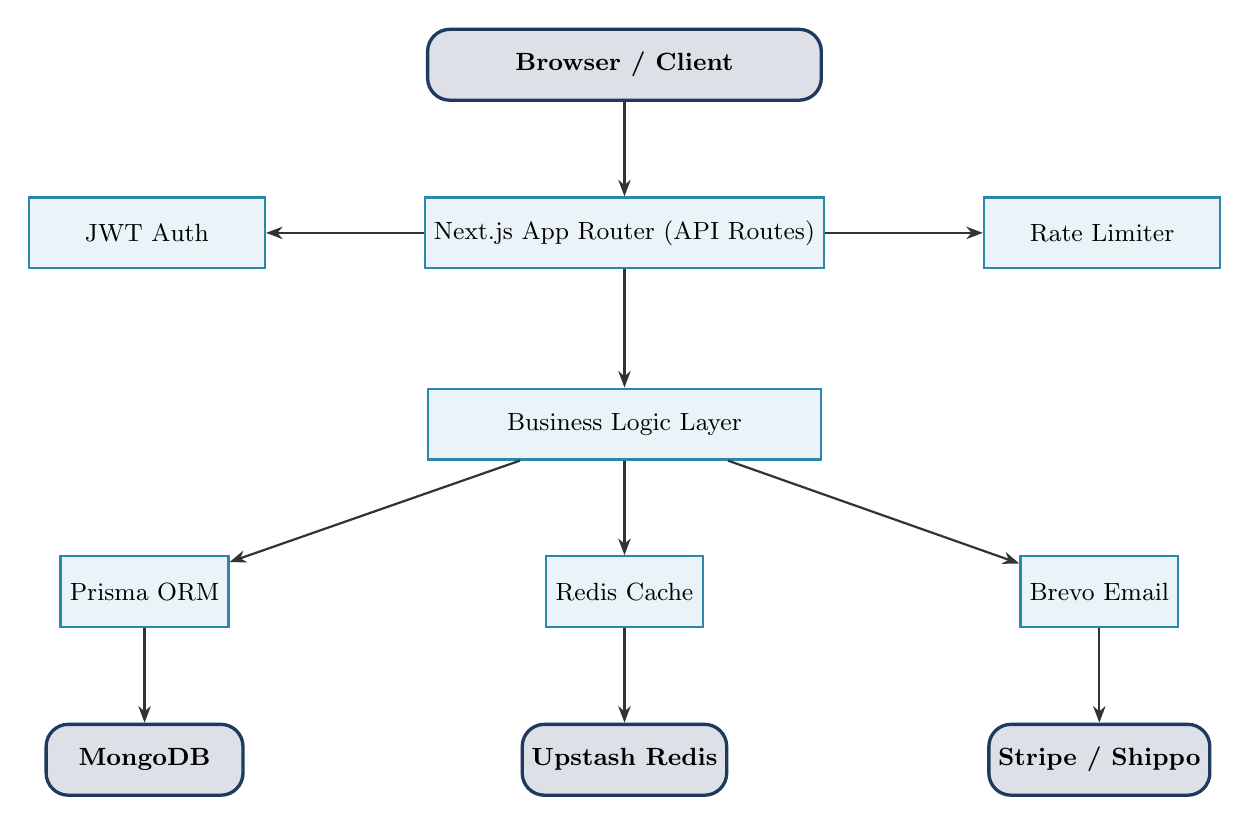
\begin{tikzpicture}[node distance=1.2cm, every node/.style={font=\small}]

  % Client Layer
  \node[startstop, minimum width=5cm] (browser) {Browser / Client};

  % API Layer
  \node[process, minimum width=5cm, below=of browser] (nextjs) {Next.js App Router (API Routes)};

  % Middleware
  \node[process, minimum width=3cm, right=2cm of nextjs] (ratelimit) {Rate Limiter};
  \node[process, minimum width=3cm, left=2cm of nextjs] (auth) {JWT Auth};

  % Business Logic
  \node[process, minimum width=5cm, below=1.5cm of nextjs] (bizlogic) {Business Logic Layer};

  % Services
  \node[process, minimum width=2cm, below left=1.2cm and 2.5cm of bizlogic] (prisma) {Prisma ORM};
  \node[process, minimum width=2cm, below=1.2cm of bizlogic] (cache) {Redis Cache};
  \node[process, minimum width=2cm, below right=1.2cm and 2.5cm of bizlogic] (email) {Brevo Email};

  % DB
  \node[startstop, minimum width=2.5cm, below=1.2cm of prisma] (mongo) {MongoDB};
  \node[startstop, minimum width=2.5cm, below=1.2cm of cache] (upstash) {Upstash Redis};
  \node[startstop, minimum width=2.5cm, below=1.2cm of email] (stripe) {Stripe / Shippo};

  % Arrows
  \draw[arrow] (browser) -- (nextjs);
  \draw[arrow] (nextjs) -- (auth);
  \draw[arrow] (nextjs) -- (ratelimit);
  \draw[arrow] (nextjs) -- (bizlogic);
  \draw[arrow] (bizlogic) -- (prisma);
  \draw[arrow] (bizlogic) -- (cache);
  \draw[arrow] (bizlogic) -- (email);
  \draw[arrow] (prisma) -- (mongo);
  \draw[arrow] (cache) -- (upstash);
  \draw[arrow] (email) -- (stripe);

\end{tikzpicture}
\caption{High-level system architecture of Stockly}
\end{figure}


% ══════════════════════════════════════════════════════════════════════════════

\chapter{Module 1: Authentication \& Session Management}
% ══════════════════════════════════════════════════════════════════════════════

\textbf{Source Files:} \texttt{utils/auth.ts}, \texttt{app/api/auth/login/route.ts}

\section{Internal Logic Walkthrough}

\subsection{verifyToken --- Branch Map}

\begin{tcolorbox}[warningbox, title={Security Critical Function}]
\texttt{verifyToken} has 5 distinct branches. All must be covered. The JWT\_SECRET
defaults to \texttt{"your\_jwt\_secret"} if the environment variable is not set ---
this is a \textbf{critical security risk} in production.
\end{tcolorbox}

\begin{center}
\begin{tabular}{clp{7cm}}
  \toprule
  \textbf{Branch} & \textbf{Condition} & \textbf{Result} \\
  \midrule
  A & \texttt{token} is falsy, \texttt{"null"}, or \texttt{"undefined"} & \texttt{return null} \\
  B & \texttt{isServer === false} (client-side execution) & \texttt{return null} \\
  C & \texttt{jwt} is undefined or \texttt{jwt.verify} missing & \texttt{return null} \\
  D & \texttt{jwt.verify} throws (expired / invalid / malformed) & \texttt{catch} $\to$ \texttt{return null} \\
  E & \texttt{jwt.verify} succeeds & \texttt{return \{ userId \}} \\
  \bottomrule
\end{tabular}
\end{center}

\subsection{verifyToken Control Flow Diagram}

\begin{figure}[h!]
\centering
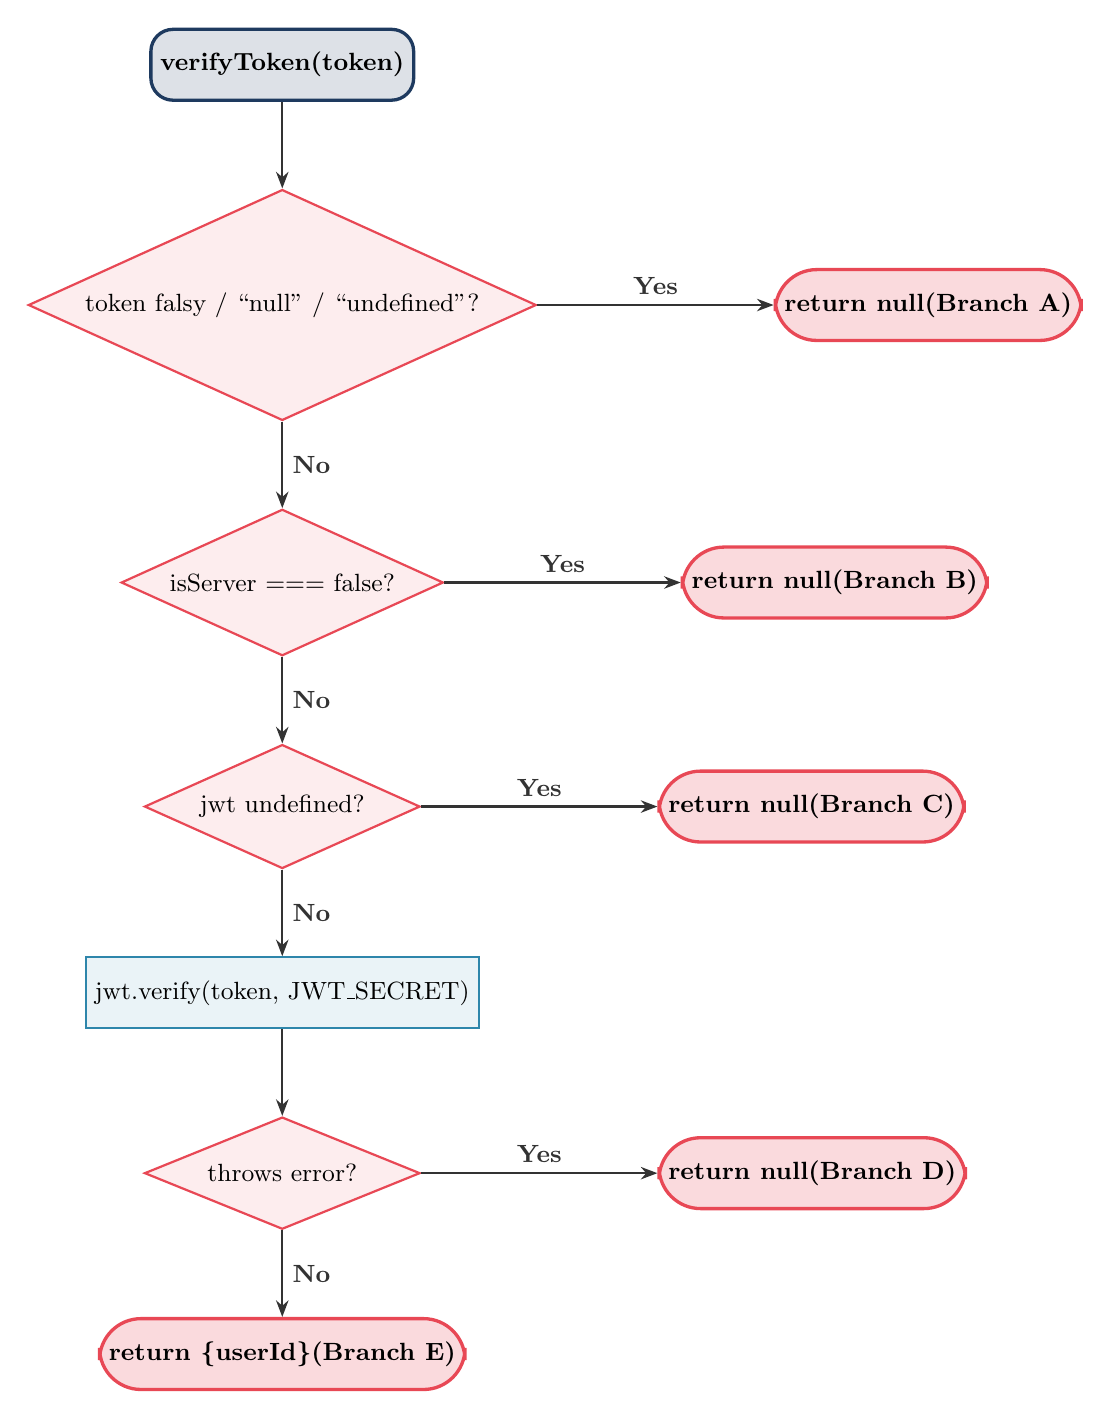
\begin{tikzpicture}[node distance=1.1cm]

  \node[startstop] (start) {verifyToken(token)};
  \node[decision, below=of start] (d1) {token falsy / ``null'' / ``undefined''?};
  \node[terminal, right=3cm of d1] (rA) {return null \\ \small(Branch A)};
  \node[decision, below=of d1] (d2) {isServer === false?};
  \node[terminal, right=3cm of d2] (rB) {return null \\ \small(Branch B)};
  \node[decision, below=of d2] (d3) {jwt undefined?};
  \node[terminal, right=3cm of d3] (rC) {return null \\ \small(Branch C)};
  \node[process, below=of d3] (verify) {jwt.verify(token, JWT\_SECRET)};
  \node[decision, below=of verify] (d4) {throws error?};
  \node[terminal, right=3cm of d4] (rD) {return null \\ \small(Branch D)};
  \node[terminal, below=of d4] (rE) {return \{userId\} \\ \small(Branch E)};

  \draw[arrow] (start) -- (d1);
  \draw[arrow] (d1) -- node[yes, above]{Yes} (rA);
  \draw[arrow] (d1) -- node[no, right]{No} (d2);
  \draw[arrow] (d2) -- node[yes, above]{Yes} (rB);
  \draw[arrow] (d2) -- node[no, right]{No} (d3);
  \draw[arrow] (d3) -- node[yes, above]{Yes} (rC);
  \draw[arrow] (d3) -- node[no, right]{No} (verify);
  \draw[arrow] (verify) -- (d4);
  \draw[arrow] (d4) -- node[yes, above]{Yes} (rD);
  \draw[arrow] (d4) -- node[no, right]{No} (rE);

\end{tikzpicture}
\caption{Control flow diagram for \texttt{verifyToken}}
\end{figure}

\subsection{Login Route Decision Tree}

\begin{figure}[h!]
\centering
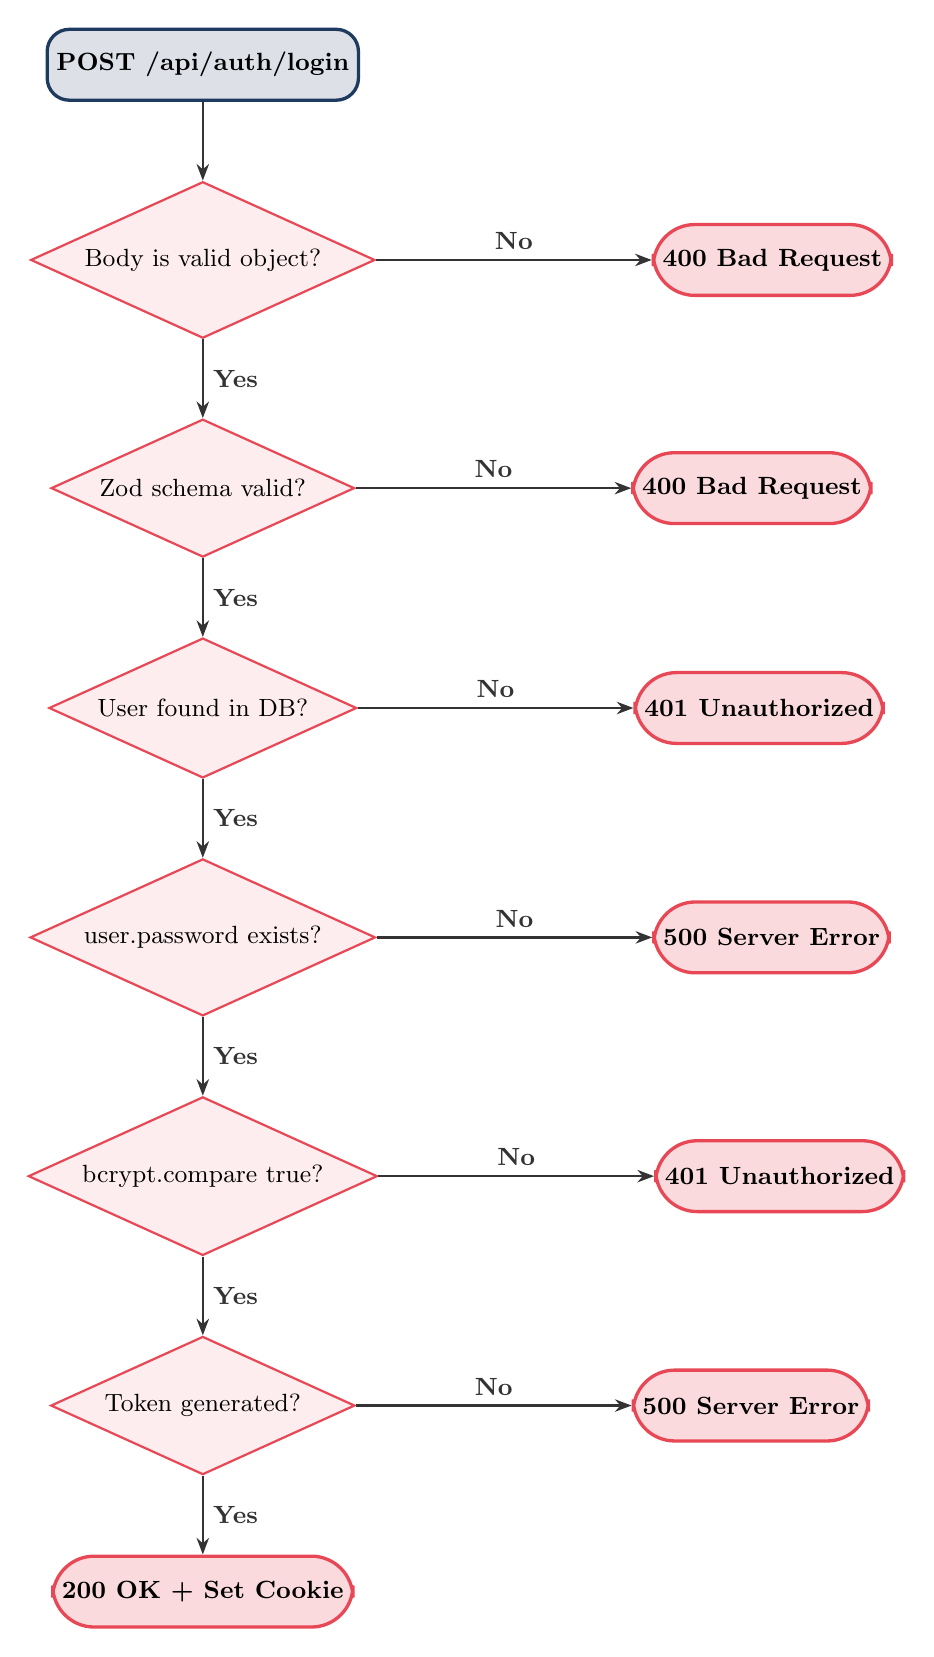
\begin{tikzpicture}[node distance=1.0cm]

  \node[startstop] (start) {POST /api/auth/login};
  \node[decision, below=of start] (d1) {Body is valid object?};
  \node[terminal, right=3.5cm of d1] (r400a) {400 Bad Request};
  \node[decision, below=of d1] (d2) {Zod schema valid?};
  \node[terminal, right=3.5cm of d2] (r400b) {400 Bad Request};
  \node[decision, below=of d2] (d3) {User found in DB?};
  \node[terminal, right=3.5cm of d3] (r401a) {401 Unauthorized};
  \node[decision, below=of d3] (d4) {user.password exists?};
  \node[terminal, right=3.5cm of d4] (r500a) {500 Server Error};
  \node[decision, below=of d4] (d5) {bcrypt.compare true?};
  \node[terminal, right=3.5cm of d5] (r401b) {401 Unauthorized};
  \node[decision, below=of d5] (d6) {Token generated?};
  \node[terminal, right=3.5cm of d6] (r500b) {500 Server Error};
  \node[terminal, below=of d6] (r200) {200 OK + Set Cookie};

  \draw[arrow] (start) -- (d1);
  \draw[arrow] (d1) -- node[no, above]{No} (r400a);
  \draw[arrow] (d1) -- node[yes, right]{Yes} (d2);
  \draw[arrow] (d2) -- node[no, above]{No} (r400b);
  \draw[arrow] (d2) -- node[yes, right]{Yes} (d3);
  \draw[arrow] (d3) -- node[no, above]{No} (r401a);
  \draw[arrow] (d3) -- node[yes, right]{Yes} (d4);
  \draw[arrow] (d4) -- node[no, above]{No} (r500a);
  \draw[arrow] (d4) -- node[yes, right]{Yes} (d5);
  \draw[arrow] (d5) -- node[no, above]{No} (r401b);
  \draw[arrow] (d5) -- node[yes, right]{Yes} (d6);
  \draw[arrow] (d6) -- node[no, above]{No} (r500b);
  \draw[arrow] (d6) -- node[yes, right]{Yes} (r200);

\end{tikzpicture}
\caption{Login route complete decision tree}
\end{figure}

\section{Test Cases --- Authentication}

\begin{tcolorbox}[testbox, title={AUTH-001 \hfill \pone}]
\textbf{Function:} \texttt{verifyToken} \\
\textbf{Scenario:} Token is an empty string \\
\textbf{Input:} \texttt{token = ""} \\
\textbf{Expected Path:} Branch A (falsy check) $\to$ \texttt{return null} \\
\textbf{Expected Output:} \texttt{null} \\
\textbf{Coverage:} Statement + Branch A
\end{tcolorbox}

\begin{tcolorbox}[testbox, title={AUTH-002 \hfill \pone}]
\textbf{Function:} \texttt{verifyToken} \\
\textbf{Scenario:} Token is the string \texttt{"null"} \\
\textbf{Input:} \texttt{token = "null"} \\
\textbf{Expected Path:} Branch A (string \texttt{"null"} check) $\to$ \texttt{return null} \\
\textbf{Expected Output:} \texttt{null} \\
\textbf{Coverage:} Branch A edge case
\end{tcolorbox}

\begin{tcolorbox}[testbox, title={AUTH-003 \hfill \pone}]
\textbf{Function:} \texttt{verifyToken} \\
\textbf{Scenario:} Token is the string \texttt{"undefined"} \\
\textbf{Input:} \texttt{token = "undefined"} \\
\textbf{Expected Path:} Branch A $\to$ \texttt{return null} \\
\textbf{Expected Output:} \texttt{null} \\
\textbf{Coverage:} Branch A edge case
\end{tcolorbox}

\begin{tcolorbox}[testbox, title={AUTH-004 \hfill \pone}]
\textbf{Function:} \texttt{verifyToken} \\
\textbf{Scenario:} Valid JWT token on server side \\
\textbf{Input:} Token generated by \texttt{generateToken("user123")} \\
\textbf{Expected Path:} Branch E $\to$ \texttt{return \{ userId: "user123" \}} \\
\textbf{Expected Output:} \texttt{\{ userId: "user123" \}} \\
\textbf{Coverage:} Happy path
\end{tcolorbox}

\begin{tcolorbox}[criticalbox, title={AUTH-005 \hfill \pone\ --- Expired Token}]
\textbf{Function:} \texttt{verifyToken} \\
\textbf{Scenario:} Expired JWT token \\
\textbf{Input:} Token with \texttt{expiresIn: "1ms"}, verified after 10ms delay \\
\textbf{Expected Path:} Branch D $\to$ \texttt{jwt.verify} throws \texttt{TokenExpiredError} $\to$ \texttt{return null} \\
\textbf{Expected Output:} \texttt{null} \\
\textbf{Coverage:} Exception handling branch
\end{tcolorbox}

\begin{tcolorbox}[criticalbox, title={AUTH-006 \hfill \pone\ --- Wrong Secret (Security)}]
\textbf{Function:} \texttt{verifyToken} \\
\textbf{Scenario:} Token signed with wrong secret \\
\textbf{Input:} \texttt{jwt.sign(\{ userId: "x" \}, "WRONG\_SECRET")} \\
\textbf{Expected Path:} Branch D $\to$ \texttt{jwt.verify} throws \texttt{JsonWebTokenError} $\to$ \texttt{return null} \\
\textbf{Expected Output:} \texttt{null} \\
\textbf{Coverage:} Security branch
\end{tcolorbox}

\begin{tcolorbox}[testbox, title={AUTH-007 \hfill \pone}]
\textbf{Function:} \texttt{verifyToken} \\
\textbf{Scenario:} Malformed / random string token \\
\textbf{Input:} \texttt{token = "not.a.jwt.token"} \\
\textbf{Expected Path:} Branch D $\to$ catch $\to$ \texttt{return null} \\
\textbf{Expected Output:} \texttt{null} \\
\textbf{Coverage:} Malformed input
\end{tcolorbox}

\begin{tcolorbox}[testbox, title={AUTH-008 \hfill \pone}]
\textbf{Function:} \texttt{generateToken} \\
\textbf{Scenario:} Valid userId generates a decodable token \\
\textbf{Input:} \texttt{userId = "abc123"} \\
\textbf{Expected:} \texttt{jwt.decode(result).userId === "abc123"} \\
\textbf{Coverage:} Token payload integrity
\end{tcolorbox}

\begin{tcolorbox}[testbox, title={AUTH-009 \hfill \pone}]
\textbf{Function:} \texttt{hashPassword} + \texttt{comparePassword} \\
\textbf{Scenario:} Hash then compare same password (round-trip) \\
\textbf{Input:} \texttt{password = "SecurePass123!"} \\
\textbf{Steps:} (1) \texttt{hash = await hashPassword(password)} \quad (2) \texttt{result = await comparePassword(password, hash)} \\
\textbf{Expected:} \texttt{result === true} \\
\textbf{Coverage:} Round-trip password verification
\end{tcolorbox}

\begin{tcolorbox}[testbox, title={AUTH-010 \hfill \pone}]
\textbf{Function:} \texttt{comparePassword} \\
\textbf{Scenario:} Wrong password against valid hash \\
\textbf{Input:} \texttt{comparePassword("WrongPass", hashOf("CorrectPass"))} \\
\textbf{Expected:} \texttt{false} \\
\textbf{Coverage:} Negative comparison branch
\end{tcolorbox}

\begin{tcolorbox}[testbox, title={AUTH-011 \hfill \pone}]
\textbf{Route:} \texttt{POST /api/auth/login} \\
\textbf{Scenario:} Missing email field in body \\
\textbf{Input:} \texttt{\{ password: "test123" \}} \\
\textbf{Expected Path:} \texttt{loginSchema.parse} throws \texttt{ZodError} $\to$ 400 \\
\textbf{Expected Response:} \texttt{\{ error: "..." \}}, status \textbf{400} \\
\textbf{Coverage:} Zod validation branch
\end{tcolorbox}

\begin{tcolorbox}[testbox, title={AUTH-012 \hfill \pone}]
\textbf{Route:} \texttt{POST /api/auth/login} \\
\textbf{Scenario:} User not found in database \\
\textbf{Input:} \texttt{\{ email: "nonexistent@test.com", password: "pass" \}} \\
\textbf{Mock:} \texttt{prisma.user.findUnique} returns \texttt{null} \\
\textbf{Expected Path:} \texttt{user === null} $\to$ 401 \\
\textbf{Expected Response:} \texttt{\{ error: "Invalid email or password" \}}, status \textbf{401} \\
\textbf{Coverage:} User not found branch
\end{tcolorbox}

\begin{tcolorbox}[criticalbox, title={AUTH-013 \hfill \ptwo\ --- Corrupted Data}]
\textbf{Route:} \texttt{POST /api/auth/login} \\
\textbf{Scenario:} User found but \texttt{password} field is \texttt{null} \\
\textbf{Mock:} \texttt{prisma.user.findUnique} returns \texttt{\{ id: "x", password: null \}} \\
\textbf{Expected Path:} \texttt{!user.password} $\to$ 500 \\
\textbf{Expected Response:} \texttt{\{ error: "User data corrupted: password missing" \}}, status \textbf{500} \\
\textbf{Coverage:} Data corruption branch
\end{tcolorbox}

\begin{tcolorbox}[testbox, title={AUTH-014 \hfill \pone}]
\textbf{Route:} \texttt{POST /api/auth/login} \\
\textbf{Scenario:} Correct credentials --- full happy path \\
\textbf{Input:} \texttt{\{ email: "admin@test.com", password: "correct" \}} \\
\textbf{Mock:} User found, \texttt{bcrypt.compare} returns \texttt{true} \\
\textbf{Expected Response:} Status \textbf{200}, \texttt{Set-Cookie} header with \texttt{session\_id} \\
\textbf{Coverage:} Full happy path
\end{tcolorbox}

\begin{tcolorbox}[testbox, title={AUTH-015 \hfill \pone}]
\textbf{Function:} \texttt{getSessionFromRequest} \\
\textbf{Scenario:} No \texttt{session\_id} cookie present \\
\textbf{Input:} Request with no cookies \\
\textbf{Expected Path:} \texttt{cookie === undefined} $\to$ \texttt{return null} \\
\textbf{Expected Output:} \texttt{null} \\
\textbf{Coverage:} Missing cookie branch
\end{tcolorbox}

\begin{tcolorbox}[testbox, title={AUTH-016 \hfill \ptwo}]
\textbf{Function:} \texttt{getSessionFromRequest} \\
\textbf{Scenario:} Valid cookie but user deleted from DB \\
\textbf{Mock:} \texttt{prisma.user.findUnique} returns \texttt{null} \\
\textbf{Expected Path:} Decoded OK $\to$ DB query $\to$ \texttt{null} \\
\textbf{Expected Output:} \texttt{null} \\
\textbf{Coverage:} Deleted user edge case
\end{tcolorbox}


% ══════════════════════════════════════════════════════════════════════════════

\chapter{Module 2: Order Management \& Stock State Machine}
% ══════════════════════════════════════════════════════════════════════════════

\textbf{Source Files:} \texttt{prisma/order.ts}, \texttt{app/api/orders/route.ts}

\section{Stock Reservation State Machine}

\begin{tcolorbox}[criticalbox, title={Critical Business Logic --- Stock Reservation}]
\begin{itemize}
  \item \textbf{Order CREATE (pending):} \texttt{reservedQuantity} \textbf{INCREASES} (stock reserved, not deducted)
  \item \textbf{Order CONFIRM / PAY:} \texttt{quantity} \textbf{DECREASES}, \texttt{reservedQuantity} \textbf{DECREASES}
  \item \textbf{Order CANCEL (was pending):} \texttt{reservedQuantity} \textbf{DECREASES} (reservation released)
  \item \textbf{Order CANCEL (was confirmed/paid):} \texttt{quantity} \textbf{INCREASES} (stock restored)
  \item \textbf{Available Stock Formula:} $\text{availableStock} = \text{quantity} - \text{reservedQuantity}$
\end{itemize}
\end{tcolorbox}

\subsection{Order Status State Machine Diagram}

\begin{figure}[h!]
\centering
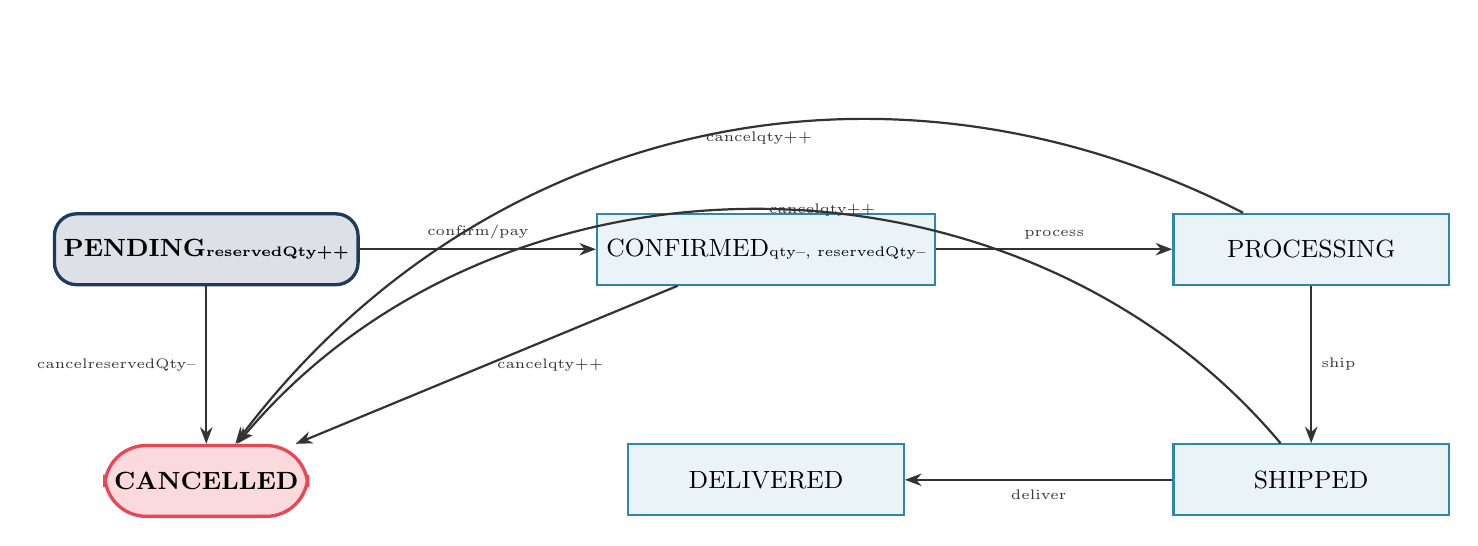
\begin{tikzpicture}[node distance=1.8cm, every node/.style={font=\small}]

  \node[startstop] (pending) {PENDING \\ \tiny reservedQty++};
  \node[process, right=3cm of pending] (confirmed) {CONFIRMED \\ \tiny qty--, reservedQty--};
  \node[process, right=3cm of confirmed] (processing) {PROCESSING};
  \node[process, below=2cm of processing] (shipped) {SHIPPED};
  \node[process, below=2cm of confirmed] (delivered) {DELIVERED};
  \node[terminal, below=2cm of pending] (cancelled) {CANCELLED};

  \draw[arrow] (pending) -- node[above]{\tiny confirm/pay} (confirmed);
  \draw[arrow] (confirmed) -- node[above]{\tiny process} (processing);
  \draw[arrow] (processing) -- node[right]{\tiny ship} (shipped);
  \draw[arrow] (shipped) -- node[below]{\tiny deliver} (delivered);
  \draw[arrow] (pending) -- node[left]{\tiny cancel \\ \tiny reservedQty--} (cancelled);
  \draw[arrow] (confirmed) -- node[right]{\tiny cancel \\ \tiny qty++} (cancelled);
  \draw[arrow] (processing) to[bend right=40] node[right]{\tiny cancel \\ \tiny qty++} (cancelled);
  \draw[arrow] (shipped) to[bend right=50] node[right]{\tiny cancel \\ \tiny qty++} (cancelled);

\end{tikzpicture}
\caption{Order status state machine with stock side-effects}
\end{figure}

\subsection{createOrder Control Flow Diagram}

\begin{figure}[h!]
\centering
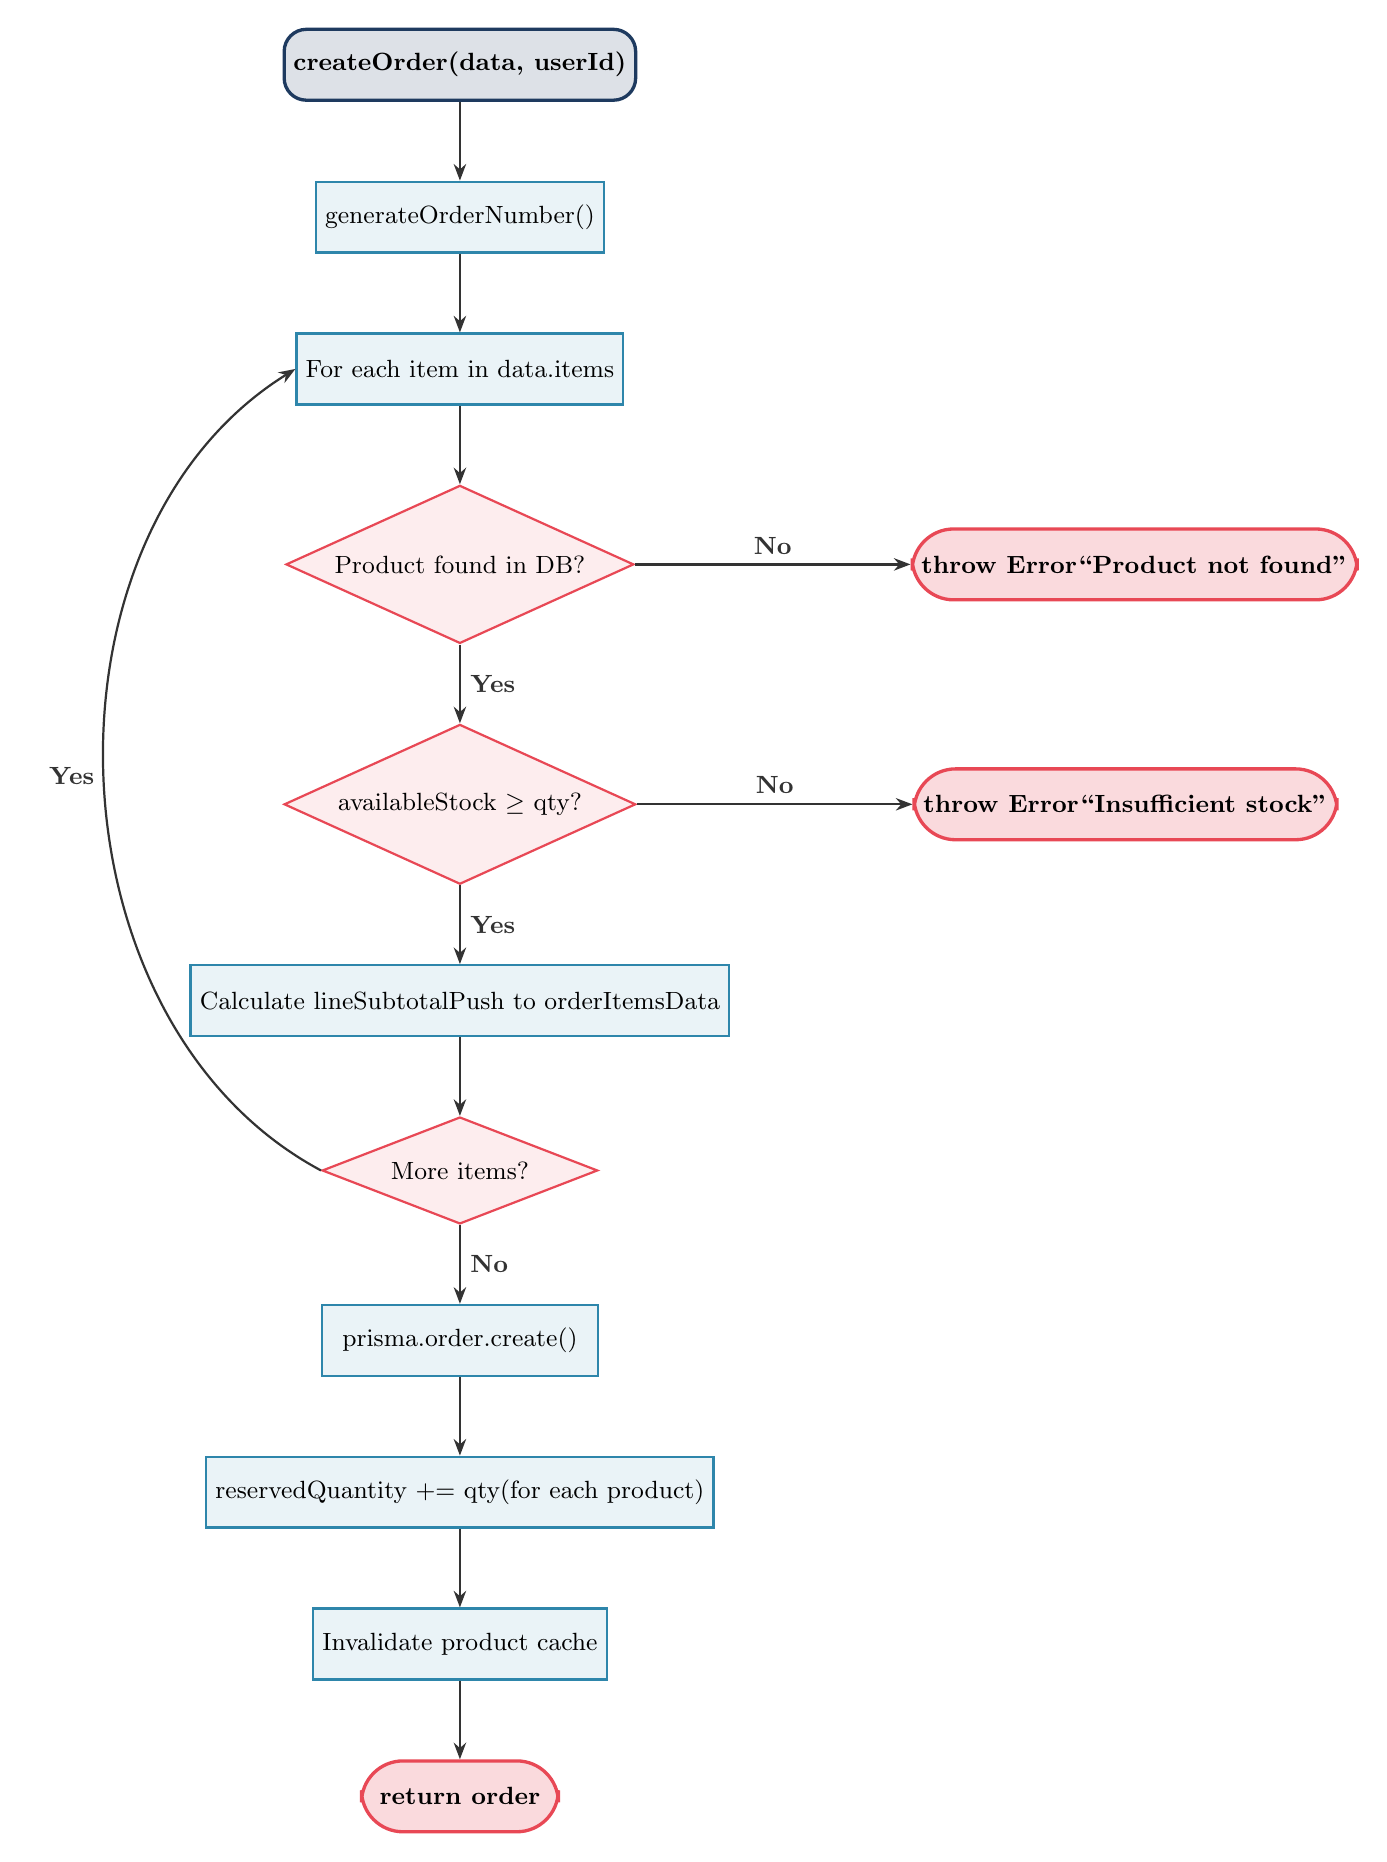
\begin{tikzpicture}[node distance=1.0cm]

  \node[startstop] (start) {createOrder(data, userId)};
  \node[process, below=of start] (gennum) {generateOrderNumber()};
  \node[process, below=of gennum] (loop) {For each item in data.items};
  \node[decision, below=of loop] (d1) {Product found in DB?};
  \node[terminal, right=3.5cm of d1] (err1) {throw Error \\ ``Product not found''};
  \node[decision, below=of d1] (d2) {availableStock $\geq$ qty?};
  \node[terminal, right=3.5cm of d2] (err2) {throw Error \\ ``Insufficient stock''};
  \node[process, below=of d2] (calc) {Calculate lineSubtotal \\ Push to orderItemsData};
  \node[decision, below=of calc] (d3) {More items?};
  \node[process, below=of d3] (create) {prisma.order.create()};
  \node[process, below=of create] (reserve) {reservedQuantity += qty \\ (for each product)};
  \node[process, below=of reserve] (cache) {Invalidate product cache};
  \node[terminal, below=of cache] (ret) {return order};

  \draw[arrow] (start) -- (gennum);
  \draw[arrow] (gennum) -- (loop);
  \draw[arrow] (loop) -- (d1);
  \draw[arrow] (d1) -- node[no, above]{No} (err1);
  \draw[arrow] (d1) -- node[yes, right]{Yes} (d2);
  \draw[arrow] (d2) -- node[no, above]{No} (err2);
  \draw[arrow] (d2) -- node[yes, right]{Yes} (calc);
  \draw[arrow] (calc) -- (d3);
  \draw[arrow] (d3.west) to[bend left=60] node[yes, left]{Yes} (loop.west);
  \draw[arrow] (d3) -- node[no, right]{No} (create);
  \draw[arrow] (create) -- (reserve);
  \draw[arrow] (reserve) -- (cache);
  \draw[arrow] (cache) -- (ret);

\end{tikzpicture}
\caption{createOrder complete control flow}
\end{figure}

\section{Test Cases --- Order Management}

\begin{tcolorbox}[testbox, title={ORD-001 \hfill \ptwo}]
\textbf{Function:} \texttt{generateOrderNumber} \\
\textbf{Scenario:} First order of the day (0 existing orders today) \\
\textbf{Mock:} \texttt{prisma.order.count} returns \texttt{0} \\
\textbf{Expected:} Sequence part = \texttt{"0001"}, format: \texttt{ORD-2026-0401-HHMMSS-0001} \\
\textbf{Coverage:} Sequence generation, zero-count branch
\end{tcolorbox}

\begin{tcolorbox}[testbox, title={ORD-002 \hfill \pthree\ --- Boundary}]
\textbf{Function:} \texttt{generateOrderNumber} \\
\textbf{Scenario:} 9999 orders already exist today \\
\textbf{Mock:} \texttt{prisma.order.count} returns \texttt{9999} \\
\textbf{Expected:} Sequence = \texttt{"10000"} (5 digits, overflow of 4-digit pad) \\
\textbf{Note:} Race condition possible under high concurrency --- not atomic \\
\textbf{Coverage:} Boundary value, sequence overflow
\end{tcolorbox}

\begin{tcolorbox}[criticalbox, title={ORD-003 \hfill \pone\ --- Product Not Found}]
\textbf{Function:} \texttt{createOrder} \\
\textbf{Scenario:} Product not found in database \\
\textbf{Input:} \texttt{data.items = [\{ productId: "nonexistent", quantity: 1 \}]} \\
\textbf{Mock:} \texttt{prisma.product.findUnique} returns \texttt{null} \\
\textbf{Expected:} \texttt{throw Error("Product not found: nonexistent")} \\
\textbf{Coverage:} Product not found branch
\end{tcolorbox}

\begin{tcolorbox}[criticalbox, title={ORD-004 \hfill \pone\ --- Insufficient Stock}]
\textbf{Function:} \texttt{createOrder} \\
\textbf{Scenario:} Insufficient available stock \\
\textbf{Input:} \texttt{item.quantity = 10} \\
\textbf{Mock:} \texttt{product.quantity = 15}, \texttt{product.reservedQuantity = 8} \\
\textbf{Internal:} $\text{availableStock} = 15 - 8 = 7 < 10$ \\
\textbf{Expected:} \texttt{throw Error("Insufficient stock. Available: 7, Requested: 10")} \\
\textbf{Coverage:} Stock check branch (insufficient)
\end{tcolorbox}

\begin{tcolorbox}[testbox, title={ORD-005 \hfill \pone\ --- Exact Stock Boundary}]
\textbf{Function:} \texttt{createOrder} \\
\textbf{Scenario:} Exactly enough stock (boundary value) \\
\textbf{Input:} \texttt{item.quantity = 7} \\
\textbf{Mock:} \texttt{product.quantity = 15}, \texttt{product.reservedQuantity = 8} \\
\textbf{Internal:} $\text{availableStock} = 7 = 7$ (exactly enough) \\
\textbf{Expected:} Order created successfully, no error \\
\textbf{Coverage:} Boundary value (exact stock match)
\end{tcolorbox}

\begin{tcolorbox}[criticalbox, title={ORD-006 \hfill \pone\ --- Boundary + 1}]
\textbf{Function:} \texttt{createOrder} \\
\textbf{Scenario:} One more than available stock \\
\textbf{Input:} \texttt{item.quantity = 8} \\
\textbf{Mock:} \texttt{product.quantity = 15}, \texttt{product.reservedQuantity = 8} \\
\textbf{Internal:} $\text{availableStock} = 7 < 8$ \\
\textbf{Expected:} \texttt{throw Error("Insufficient stock")} \\
\textbf{Coverage:} Boundary value + 1
\end{tcolorbox}

\begin{tcolorbox}[testbox, title={ORD-007 \hfill \ptwo}]
\textbf{Function:} \texttt{createOrder} \\
\textbf{Scenario:} \texttt{reservedQuantity} is \texttt{null} (not yet set) \\
\textbf{Mock:} \texttt{product.quantity = 10}, \texttt{product.reservedQuantity = null} \\
\textbf{Internal:} $\text{availableStock} = 10 - \texttt{Number(null)} = 10 - 0 = 10$ \\
\textbf{Expected:} \texttt{availableStock} correctly computed as \texttt{10} \\
\textbf{Coverage:} Null coalescing in stock calculation
\end{tcolorbox}

\begin{tcolorbox}[criticalbox, title={ORD-008 \hfill \pone\ --- Atomicity Gap}]
\textbf{Function:} \texttt{createOrder} \\
\textbf{Scenario:} Multiple items, second item fails stock check \\
\textbf{Input:} \texttt{items = [\{ productA, qty: 1 \}, \{ productB, qty: 999 \}]} \\
\textbf{Mock:} productA has stock, productB has only 5 \\
\textbf{Expected:} Error thrown on productB; \textbf{NO} reservation made for productA \\
\textbf{Note:} Tests fail-fast behaviour before any DB writes \\
\textbf{Coverage:} Partial failure rollback (atomicity check)
\end{tcolorbox}

\begin{tcolorbox}[testbox, title={ORD-009 \hfill \pone}]
\textbf{Function:} \texttt{createOrder} \\
\textbf{Scenario:} Tax, shipping, discount all provided \\
\textbf{Input:} \texttt{subtotal=100, tax=10, shipping=5, discount=15} \\
\textbf{Expected:} $\text{total} = 100 + 10 + 5 - 15 = 100$ \\
\textbf{Coverage:} Total calculation formula
\end{tcolorbox}

\begin{tcolorbox}[testbox, title={ORD-010 \hfill \ptwo}]
\textbf{Function:} \texttt{createOrder} \\
\textbf{Scenario:} Tax and shipping are 0 (falsy) \\
\textbf{Input:} \texttt{tax=0, shipping=0, discount=0} \\
\textbf{Internal:} \texttt{tax > 0} is \texttt{false} $\to$ stored as \texttt{null} \\
\textbf{Expected:} \texttt{order.tax = null}, \texttt{order.shipping = null}, \texttt{order.discount = null} \\
\textbf{Coverage:} Falsy-to-null conversion branches
\end{tcolorbox}

\begin{tcolorbox}[testbox, title={ORD-011 \hfill \pone}]
\textbf{Function:} \texttt{createOrder} \\
\textbf{Scenario:} Verify \texttt{reservedQuantity} incremented after order creation \\
\textbf{Input:} Single item, \texttt{quantity = 3} \\
\textbf{Mock:} \texttt{product.reservedQuantity = 5} before order \\
\textbf{Expected:} After \texttt{createOrder}, \texttt{product.reservedQuantity = 8} \\
\textbf{Coverage:} Stock reservation side effect
\end{tcolorbox}

\begin{tcolorbox}[testbox, title={ORD-012 \hfill \pone}]
\textbf{Route:} \texttt{GET /api/orders} \\
\textbf{Scenario:} Unauthenticated request (no session cookie) \\
\textbf{Mock:} \texttt{getSessionFromRequest} returns \texttt{null} \\
\textbf{Expected:} \texttt{\{ error: "Unauthorized" \}}, status \textbf{401} \\
\textbf{Coverage:} Auth guard branch
\end{tcolorbox}

\begin{tcolorbox}[testbox, title={ORD-013 \hfill \ptwo}]
\textbf{Route:} \texttt{GET /api/orders} \\
\textbf{Scenario:} Supplier role with no supplier record \\
\textbf{Mock:} \texttt{session.role = "supplier"}, \texttt{getSupplierByUserId} returns \texttt{null} \\
\textbf{Expected:} \texttt{NextResponse.json([])} --- empty array, not error \\
\textbf{Coverage:} Supplier without record branch
\end{tcolorbox}

\begin{tcolorbox}[testbox, title={ORD-014 \hfill \ptwo}]
\textbf{Route:} \texttt{GET /api/orders} \\
\textbf{Scenario:} Cache hit for orders list \\
\textbf{Mock:} \texttt{getCache} returns cached array \\
\textbf{Expected:} Returns cached data without DB query \\
\textbf{Coverage:} Cache hit branch
\end{tcolorbox}

\begin{tcolorbox}[testbox, title={ORD-015 \hfill \pone}]
\textbf{Route:} \texttt{GET /api/orders} \\
\textbf{Scenario:} Client role fetches only their orders \\
\textbf{Mock:} \texttt{session.role = "client"}, \texttt{session.id = "clientUserId"} \\
\textbf{Expected:} \texttt{getOrdersByClientId} called with \texttt{"clientUserId"} \\
\textbf{Coverage:} Role-based query branching (client)
\end{tcolorbox}

\begin{tcolorbox}[testbox, title={ORD-016 \hfill \ptwo}]
\textbf{Route:} \texttt{GET /api/orders} \\
\textbf{Scenario:} Rate limit exceeded \\
\textbf{Mock:} \texttt{withRateLimit} returns a 429 response \\
\textbf{Expected:} 429 response returned immediately, no DB query \\
\textbf{Coverage:} Rate limit early return branch
\end{tcolorbox}


% ══════════════════════════════════════════════════════════════════════════════

\chapter{Module 3: Invoice Generation \& Financial Logic}
% ══════════════════════════════════════════════════════════════════════════════

\textbf{Source Files:} \texttt{prisma/invoice.ts}, \texttt{app/api/invoices/route.ts}

\section{Internal Logic Walkthrough}

\subsection{createInvoice Control Flow Diagram}

\begin{figure}[h!]
\centering
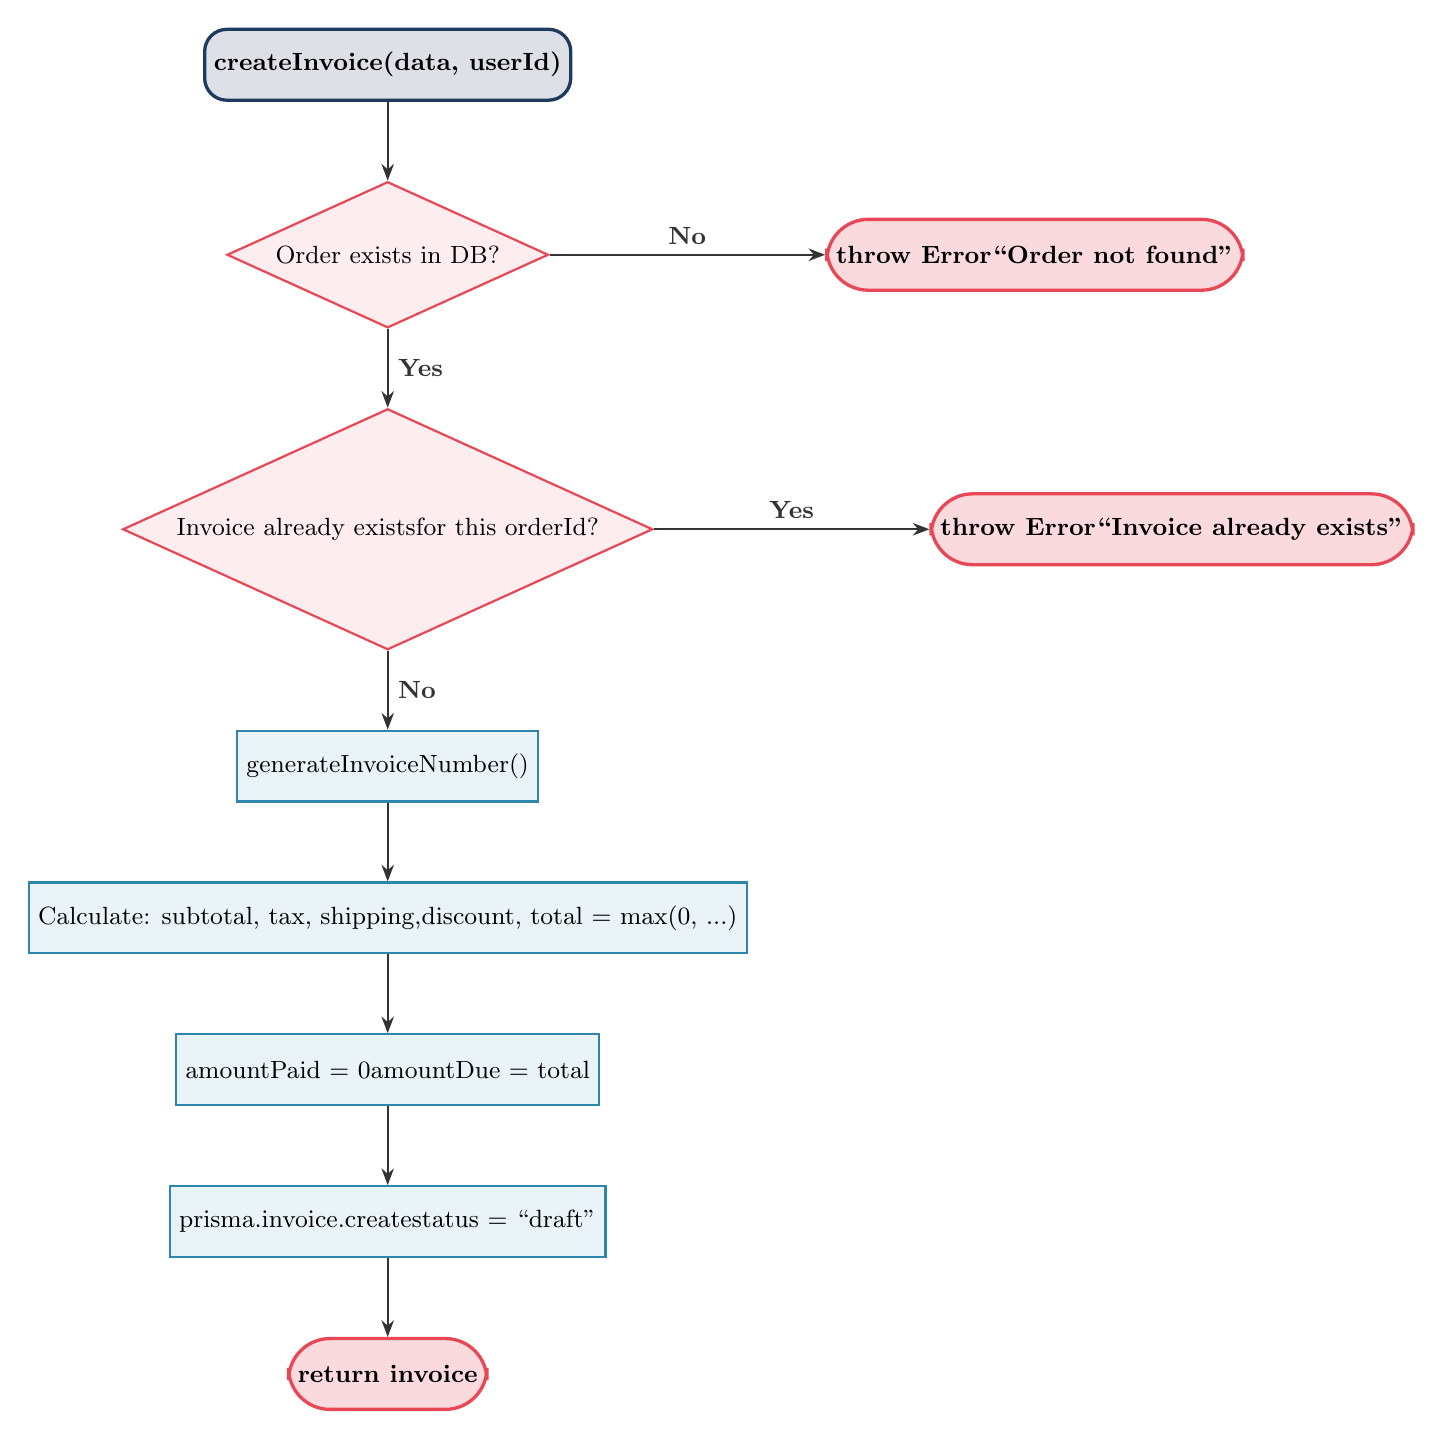
\begin{tikzpicture}[node distance=1.0cm]

  \node[startstop] (start) {createInvoice(data, userId)};
  \node[decision, below=of start] (d1) {Order exists in DB?};
  \node[terminal, right=3.5cm of d1] (err1) {throw Error \\ ``Order not found''};
  \node[decision, below=of d1] (d2) {Invoice already exists \\ for this orderId?};
  \node[terminal, right=3.5cm of d2] (err2) {throw Error \\ ``Invoice already exists''};
  \node[process, below=of d2] (gennum) {generateInvoiceNumber()};
  \node[process, below=of gennum] (calc) {Calculate: subtotal, tax, shipping, \\ discount, total = max(0, ...)};
  \node[process, below=of calc] (amounts) {amountPaid = 0 \\ amountDue = total};
  \node[process, below=of amounts] (create) {prisma.invoice.create \\ status = ``draft''};
  \node[terminal, below=of create] (ret) {return invoice};

  \draw[arrow] (start) -- (d1);
  \draw[arrow] (d1) -- node[no, above]{No} (err1);
  \draw[arrow] (d1) -- node[yes, right]{Yes} (d2);
  \draw[arrow] (d2) -- node[yes, above]{Yes} (err2);
  \draw[arrow] (d2) -- node[no, right]{No} (gennum);
  \draw[arrow] (gennum) -- (calc);
  \draw[arrow] (calc) -- (amounts);
  \draw[arrow] (amounts) -- (create);
  \draw[arrow] (create) -- (ret);

\end{tikzpicture}
\caption{createInvoice complete control flow}
\end{figure}

\subsection{generateInvoiceNumber Uniqueness Loop}

\begin{figure}[h!]
\centering
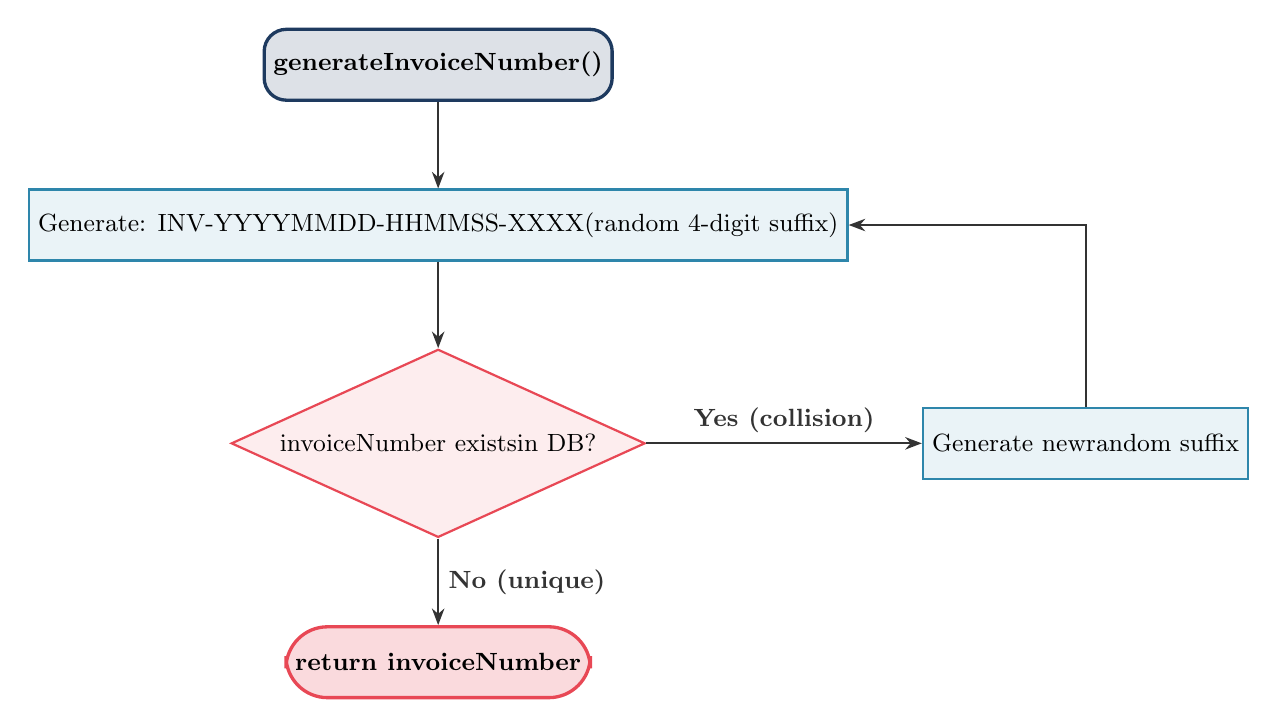
\begin{tikzpicture}[node distance=1.1cm]

  \node[startstop] (start) {generateInvoiceNumber()};
  \node[process, below=of start] (gen) {Generate: INV-YYYYMMDD-HHMMSS-XXXX \\ (random 4-digit suffix)};
  \node[decision, below=of gen] (d1) {invoiceNumber exists \\ in DB?};
  \node[process, right=3.5cm of d1] (regen) {Generate new \\ random suffix};
  \node[terminal, below=of d1] (ret) {return invoiceNumber};

  \draw[arrow] (start) -- (gen);
  \draw[arrow] (gen) -- (d1);
  \draw[arrow] (d1) -- node[yes, above]{Yes (collision)} (regen);
  \draw[arrow] (regen) |- (gen);
  \draw[arrow] (d1) -- node[no, right]{No (unique)} (ret);

\end{tikzpicture}
\caption{Invoice number uniqueness loop (collision probability = 1/9000)}
\end{figure}

\subsection{Nullish Coalescing Chain for Tax/Shipping/Discount}

\begin{tcolorbox}[infobox, title={Critical: \texttt{??} vs \texttt{||} Operator}]
The invoice uses \textbf{nullish coalescing} (\texttt{??}) not logical OR (\texttt{||}).
This means an explicit \texttt{0} from \texttt{data.tax} is \textbf{respected} and does NOT
fall back to \texttt{order.tax}. Only \texttt{null} or \texttt{undefined} trigger the fallback.

\medskip
\texttt{tax = data.tax ?? order.tax ?? 0}

\begin{center}
\begin{tabular}{lll}
  \toprule
  \texttt{data.tax} & \texttt{order.tax} & \textbf{Result} \\
  \midrule
  \texttt{20}        & \texttt{15}        & \texttt{20} (data wins) \\
  \texttt{0}         & \texttt{15}        & \texttt{0}  (explicit zero respected) \\
  \texttt{undefined} & \texttt{15}        & \texttt{15} (fallback to order) \\
  \texttt{null}      & \texttt{15}        & \texttt{15} (fallback to order) \\
  \texttt{null}      & \texttt{null}      & \texttt{0}  (final fallback) \\
  \bottomrule
\end{tabular}
\end{center}
\end{tcolorbox}

\section{Test Cases --- Invoice Generation}

\begin{tcolorbox}[testbox, title={INV-001 \hfill \ptwo}]
\textbf{Function:} \texttt{generateInvoiceNumber} \\
\textbf{Scenario:} No collision (first attempt is unique) \\
\textbf{Mock:} \texttt{prisma.invoice.findUnique} returns \texttt{null} on first call \\
\textbf{Expected:} Returns \texttt{INV-YYYYMMDD-HHMMSS-XXXX} format; while loop executes once \\
\textbf{Coverage:} Happy path, no collision
\end{tcolorbox}

\begin{tcolorbox}[testbox, title={INV-002 \hfill \ptwo}]
\textbf{Function:} \texttt{generateInvoiceNumber} \\
\textbf{Scenario:} First attempt collides, second is unique \\
\textbf{Mock:} \texttt{findUnique} returns existing invoice on call 1, \texttt{null} on call 2 \\
\textbf{Expected:} While loop executes twice, returns second generated number \\
\textbf{Coverage:} Collision handling branch (while loop iteration)
\end{tcolorbox}

\begin{tcolorbox}[testbox, title={INV-003 \hfill \ptwo}]
\textbf{Function:} \texttt{generateInvoiceNumber} \\
\textbf{Scenario:} Verify format structure \\
\textbf{Expected:} Result matches regex \texttt{/\^{}INV-\textbackslash d\{8\}-\textbackslash d\{6\}-\textbackslash d\{4\}\$/} \\
\textbf{Coverage:} Output format validation
\end{tcolorbox}

\begin{tcolorbox}[criticalbox, title={INV-004 \hfill \pone\ --- Order Not Found}]
\textbf{Function:} \texttt{createInvoice} \\
\textbf{Scenario:} Order not found \\
\textbf{Input:} \texttt{data.orderId = "nonexistent"} \\
\textbf{Mock:} \texttt{prisma.order.findUnique} returns \texttt{null} \\
\textbf{Expected:} \texttt{throw Error("Order with ID nonexistent not found")} \\
\textbf{Coverage:} Order not found branch
\end{tcolorbox}

\begin{tcolorbox}[criticalbox, title={INV-005 \hfill \pone\ --- Duplicate Invoice}]
\textbf{Function:} \texttt{createInvoice} \\
\textbf{Scenario:} Invoice already exists for this order \\
\textbf{Mock:} \texttt{prisma.invoice.findUnique} returns existing invoice \\
\textbf{Expected:} \texttt{throw Error("Invoice already exists for order \{orderId\}")} \\
\textbf{Coverage:} Duplicate invoice prevention branch
\end{tcolorbox}

\begin{tcolorbox}[testbox, title={INV-006 \hfill \pone}]
\textbf{Function:} \texttt{createInvoice} \\
\textbf{Scenario:} Total calculation with all fields \\
\textbf{Input:} \texttt{subtotal=200, tax=20, shipping=10, discount=30} \\
\textbf{Expected:} $\text{total} = \max(0,\; 200 + 20 + 10 - 30) = 200$ \\
\textbf{Coverage:} Total formula
\end{tcolorbox}

\begin{tcolorbox}[criticalbox, title={INV-007 \hfill \pone\ --- Negative Total Prevention}]
\textbf{Function:} \texttt{createInvoice} \\
\textbf{Scenario:} Discount exceeds subtotal + tax + shipping \\
\textbf{Input:} \texttt{subtotal=50, tax=5, shipping=5, discount=100} \\
\textbf{Expected:} $\text{total} = \max(0,\; 50 + 5 + 5 - 100) = \max(0, -40) = 0$ \\
\textbf{Coverage:} \texttt{Math.max(0, ...)} negative prevention branch
\end{tcolorbox}

\begin{tcolorbox}[testbox, title={INV-008 \hfill \ptwo}]
\textbf{Function:} \texttt{createInvoice} \\
\textbf{Scenario:} \texttt{data.tax} is \texttt{0} (explicit zero, not null) \\
\textbf{Input:} \texttt{data.tax = 0}, \texttt{order.tax = 15} \\
\textbf{Internal:} \texttt{tax = 0 ?? 15 = 0} \\
\textbf{Expected:} \texttt{tax = 0} (data value respected, not overridden by \texttt{order.tax}) \\
\textbf{Coverage:} Nullish coalescing vs OR operator distinction
\end{tcolorbox}

\begin{tcolorbox}[testbox, title={INV-009 \hfill \ptwo}]
\textbf{Function:} \texttt{createInvoice} \\
\textbf{Scenario:} \texttt{data.tax} is \texttt{undefined}, \texttt{order.tax} is \texttt{15} \\
\textbf{Internal:} \texttt{tax = undefined ?? 15 ?? 0 = 15} \\
\textbf{Expected:} \texttt{tax = 15} (falls back to \texttt{order.tax}) \\
\textbf{Coverage:} Fallback chain in nullish coalescing
\end{tcolorbox}

\begin{tcolorbox}[testbox, title={INV-010 \hfill \ptwo}]
\textbf{Function:} \texttt{createInvoice} \\
\textbf{Scenario:} Both \texttt{data.tax} and \texttt{order.tax} are \texttt{null} \\
\textbf{Internal:} \texttt{tax = null ?? null ?? 0 = 0} \\
\textbf{Expected:} \texttt{tax = 0} (final fallback) \\
\textbf{Coverage:} Double null fallback
\end{tcolorbox}

\begin{tcolorbox}[testbox, title={INV-011 \hfill \pone}]
\textbf{Function:} \texttt{createInvoice} \\
\textbf{Scenario:} \texttt{amountPaid} always starts at 0 \\
\textbf{Expected:} \texttt{invoice.amountPaid = 0} regardless of input; \texttt{invoice.amountDue = invoice.total} \\
\textbf{Coverage:} Initial payment state
\end{tcolorbox}

\begin{tcolorbox}[testbox, title={INV-012 \hfill \pone}]
\textbf{Function:} \texttt{createInvoice} \\
\textbf{Scenario:} Invoice status always starts as \texttt{"draft"} \\
\textbf{Expected:} \texttt{invoice.status = "draft"} \\
\textbf{Coverage:} Default status branch
\end{tcolorbox}


% ══════════════════════════════════════════════════════════════════════════════

\chapter{Module 4: Demand Forecasting Engine}
% ══════════════════════════════════════════════════════════════════════════════

\textbf{Source File:} \texttt{lib/forecasting/demand-forecast.ts}

\section{Configuration Constants}

\begin{center}
\begin{tabular}{lrl}
  \toprule
  \textbf{Constant} & \textbf{Value} & \textbf{Purpose} \\
  \midrule
  \texttt{ANALYSIS\_DAYS}     & 30  & Days of historical data to analyse \\
  \texttt{FORECAST\_DAYS}     & 14  & Days to forecast ahead \\
  \texttt{ANOMALY\_THRESHOLD} & 2.0 & Standard deviations for anomaly detection \\
  \texttt{REORDER\_LEAD\_DAYS}& 7   & Days lead time for reorder \\
  \bottomrule
\end{tabular}
\end{center}

\section{Mathematical Formulas}

\subsection{Standard Deviation (Population)}
\[
  \sigma = \sqrt{\frac{1}{N}\sum_{i=1}^{N}(x_i - \bar{x})^2}
\]

\subsection{Linear Regression Slope}
\[
  \text{slope} = \frac{n \sum x_i y_i - \sum x_i \sum y_i}{n \sum x_i^2 - (\sum x_i)^2}
\]

\subsection{Percentage Change (Trend)}
\[
  \text{percentageChange} = \frac{\text{slope} \times n \times 100}{\bar{y}} \quad (\text{if } \bar{y} > 0)
\]

\subsection{Days Until Stockout}
\[
  \text{daysUntilStockout} = \left\lfloor \frac{\text{availableStock}}{\text{predictedDailySales}} \right\rfloor \quad (\text{if predictedDailySales} > 0)
\]

\subsection{Weighted Predicted Daily Sales}
\[
  \text{predicted} = 0.7 \times \text{recentAvg} + 0.3 \times \text{overallAvg} \quad (\text{if recentDays} \geq 7)
\]

\section{analyzeTrend Control Flow Diagram}

\begin{figure}[h!]
\centering
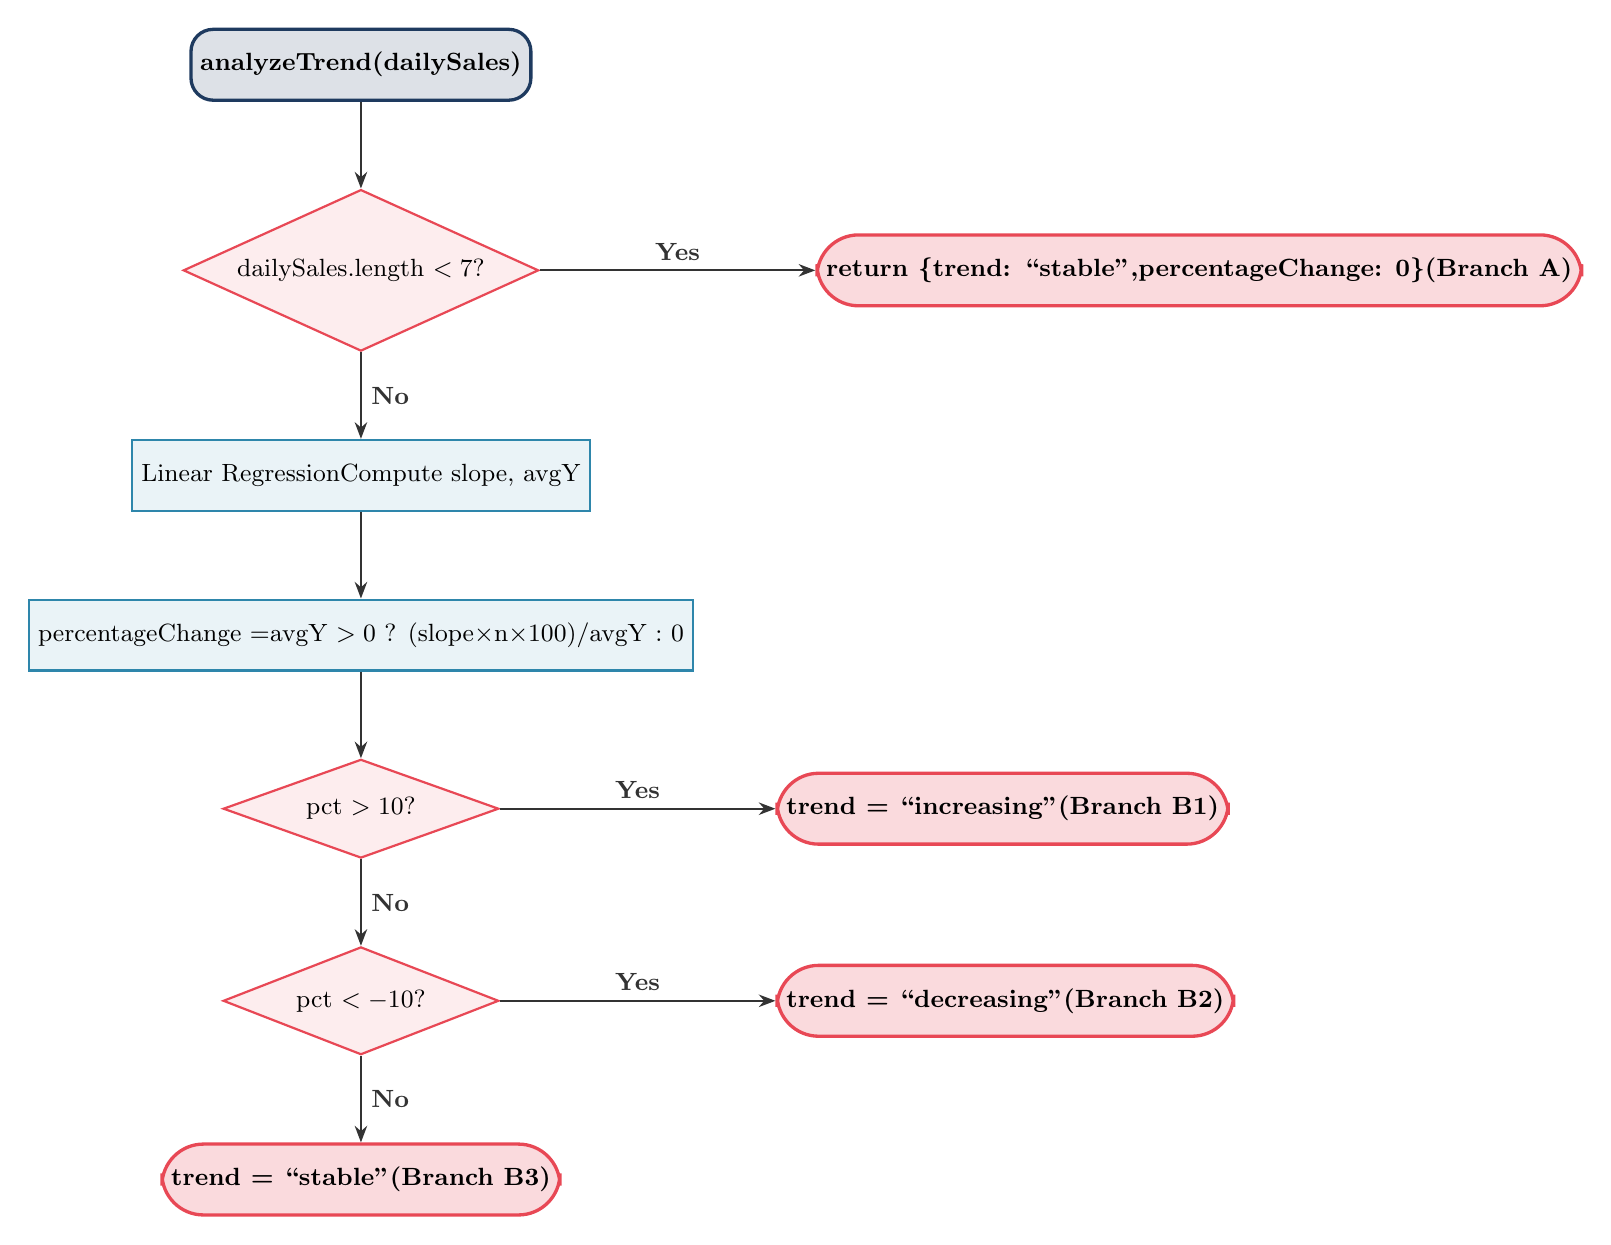
\begin{tikzpicture}[node distance=1.1cm]

  \node[startstop] (start) {analyzeTrend(dailySales)};
  \node[decision, below=of start] (d1) {dailySales.length $< 7$?};
  \node[terminal, right=3.5cm of d1] (rA) {return \{trend: ``stable'', \\ percentageChange: 0\} \\ \small(Branch A)};
  \node[process, below=of d1] (regress) {Linear Regression \\ Compute slope, avgY};
  \node[process, below=of regress] (pct) {percentageChange = \\ avgY $> 0$ ? (slope$\times$n$\times$100)/avgY : 0};
  \node[decision, below=of pct] (d2) {pct $> 10$?};
  \node[terminal, right=3.5cm of d2] (rB1) {trend = ``increasing'' \\ \small(Branch B1)};
  \node[decision, below=of d2] (d3) {pct $< -10$?};
  \node[terminal, right=3.5cm of d3] (rB2) {trend = ``decreasing'' \\ \small(Branch B2)};
  \node[terminal, below=of d3] (rB3) {trend = ``stable'' \\ \small(Branch B3)};

  \draw[arrow] (start) -- (d1);
  \draw[arrow] (d1) -- node[yes, above]{Yes} (rA);
  \draw[arrow] (d1) -- node[no, right]{No} (regress);
  \draw[arrow] (regress) -- (pct);
  \draw[arrow] (pct) -- (d2);
  \draw[arrow] (d2) -- node[yes, above]{Yes} (rB1);
  \draw[arrow] (d2) -- node[no, right]{No} (d3);
  \draw[arrow] (d3) -- node[yes, above]{Yes} (rB2);
  \draw[arrow] (d3) -- node[no, right]{No} (rB3);

\end{tikzpicture}
\caption{analyzeTrend control flow with all branches}
\end{figure}

\section{detectAnomalies Control Flow Diagram}

\begin{figure}[h!]
\centering
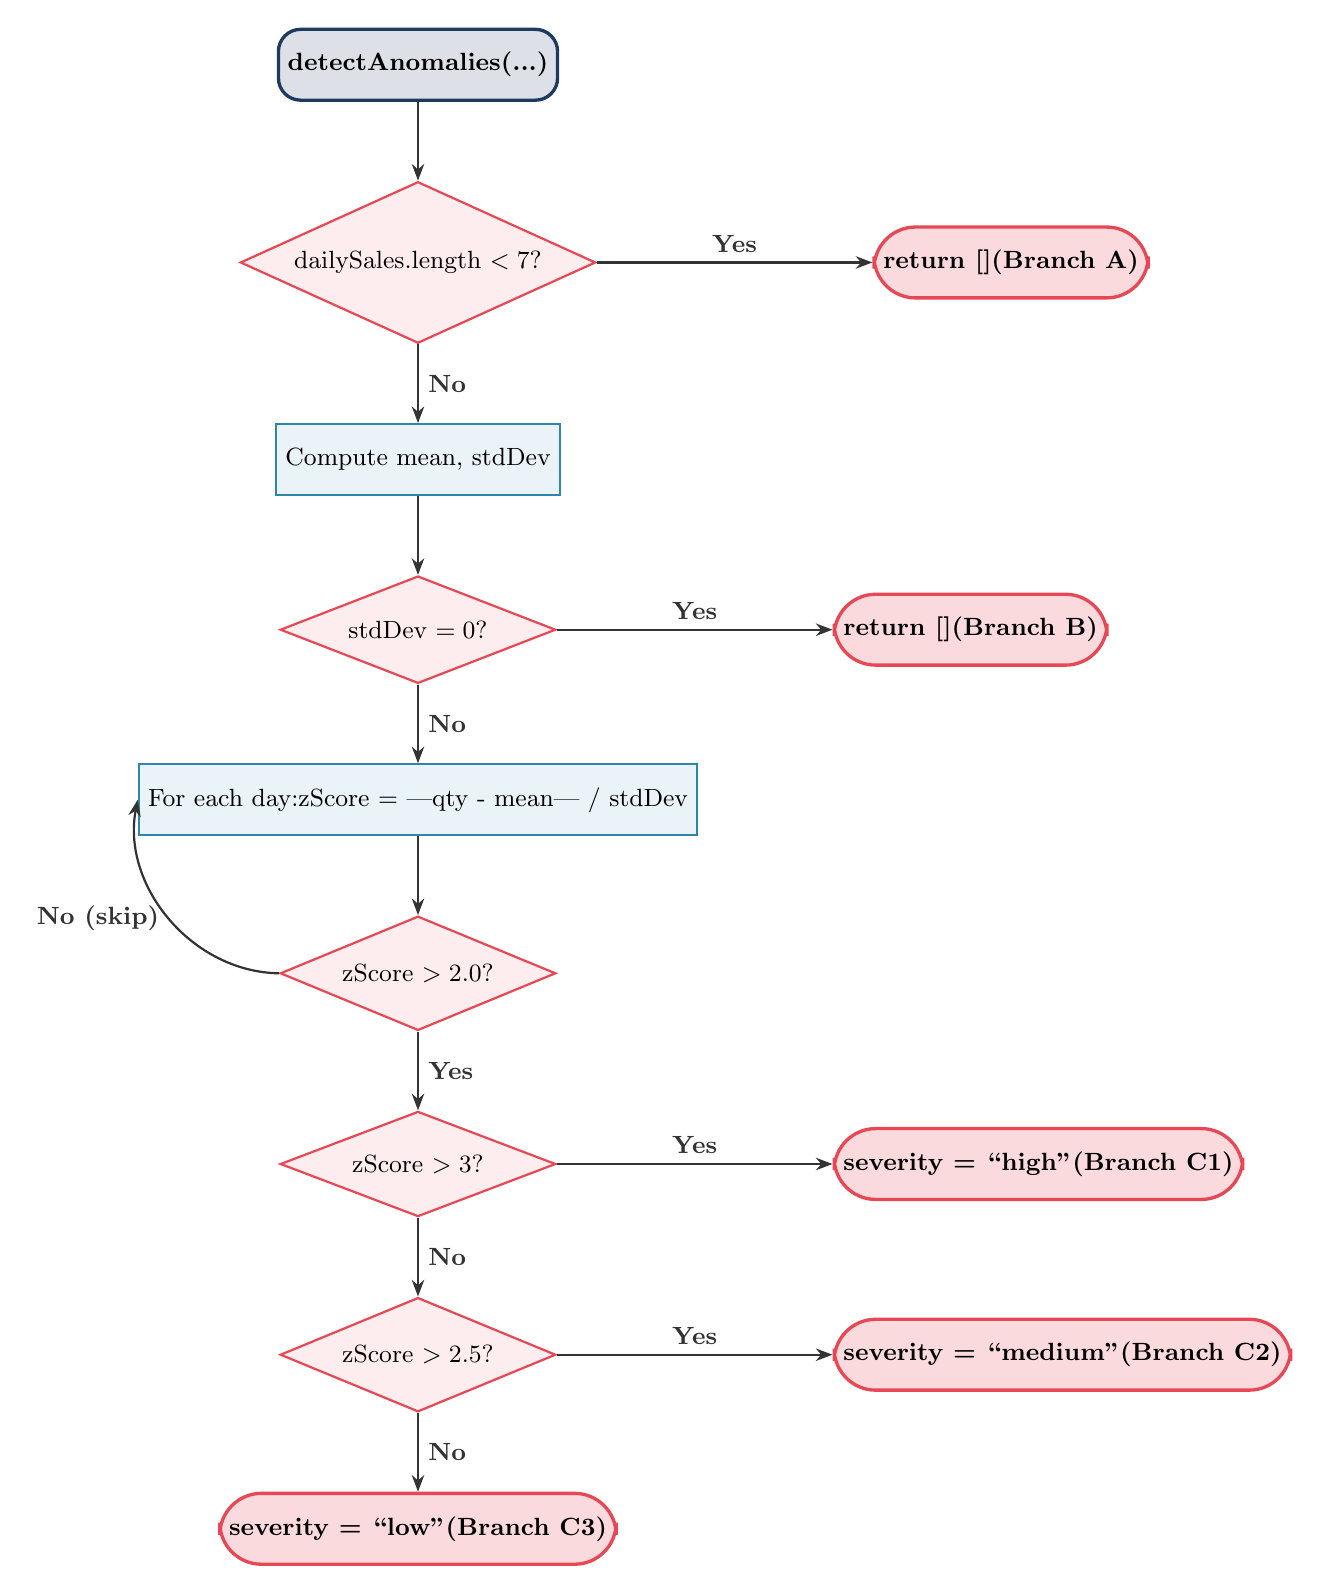
\begin{tikzpicture}[node distance=1.0cm]

  \node[startstop] (start) {detectAnomalies(...)};
  \node[decision, below=of start] (d1) {dailySales.length $< 7$?};
  \node[terminal, right=3.5cm of d1] (rA) {return [] \\ \small(Branch A)};
  \node[process, below=of d1] (stats) {Compute mean, stdDev};
  \node[decision, below=of stats] (d2) {stdDev $= 0$?};
  \node[terminal, right=3.5cm of d2] (rB) {return [] \\ \small(Branch B)};
  \node[process, below=of d2] (loop) {For each day: \\ zScore = |qty - mean| / stdDev};
  \node[decision, below=of loop] (d3) {zScore $> 2.0$?};
  \node[decision, below=of d3] (d4) {zScore $> 3$?};
  \node[terminal, right=3.5cm of d4] (rC1) {severity = ``high'' \\ \small(Branch C1)};
  \node[decision, below=of d4] (d5) {zScore $> 2.5$?};
  \node[terminal, right=3.5cm of d5] (rC2) {severity = ``medium'' \\ \small(Branch C2)};
  \node[terminal, below=of d5] (rC3) {severity = ``low'' \\ \small(Branch C3)};

  \draw[arrow] (start) -- (d1);
  \draw[arrow] (d1) -- node[yes, above]{Yes} (rA);
  \draw[arrow] (d1) -- node[no, right]{No} (stats);
  \draw[arrow] (stats) -- (d2);
  \draw[arrow] (d2) -- node[yes, above]{Yes} (rB);
  \draw[arrow] (d2) -- node[no, right]{No} (loop);
  \draw[arrow] (loop) -- (d3);
  \draw[arrow] (d3.west) to[bend left=50] node[no, left]{No (skip)} (loop.west);
  \draw[arrow] (d3) -- node[yes, right]{Yes} (d4);
  \draw[arrow] (d4) -- node[yes, above]{Yes} (rC1);
  \draw[arrow] (d4) -- node[no, right]{No} (d5);
  \draw[arrow] (d5) -- node[yes, above]{Yes} (rC2);
  \draw[arrow] (d5) -- node[no, right]{No} (rC3);

\end{tikzpicture}
\caption{detectAnomalies control flow with severity branches}
\end{figure}

\section{Reorder Recommendation Decision Diagram}

\begin{figure}[h!]
\centering
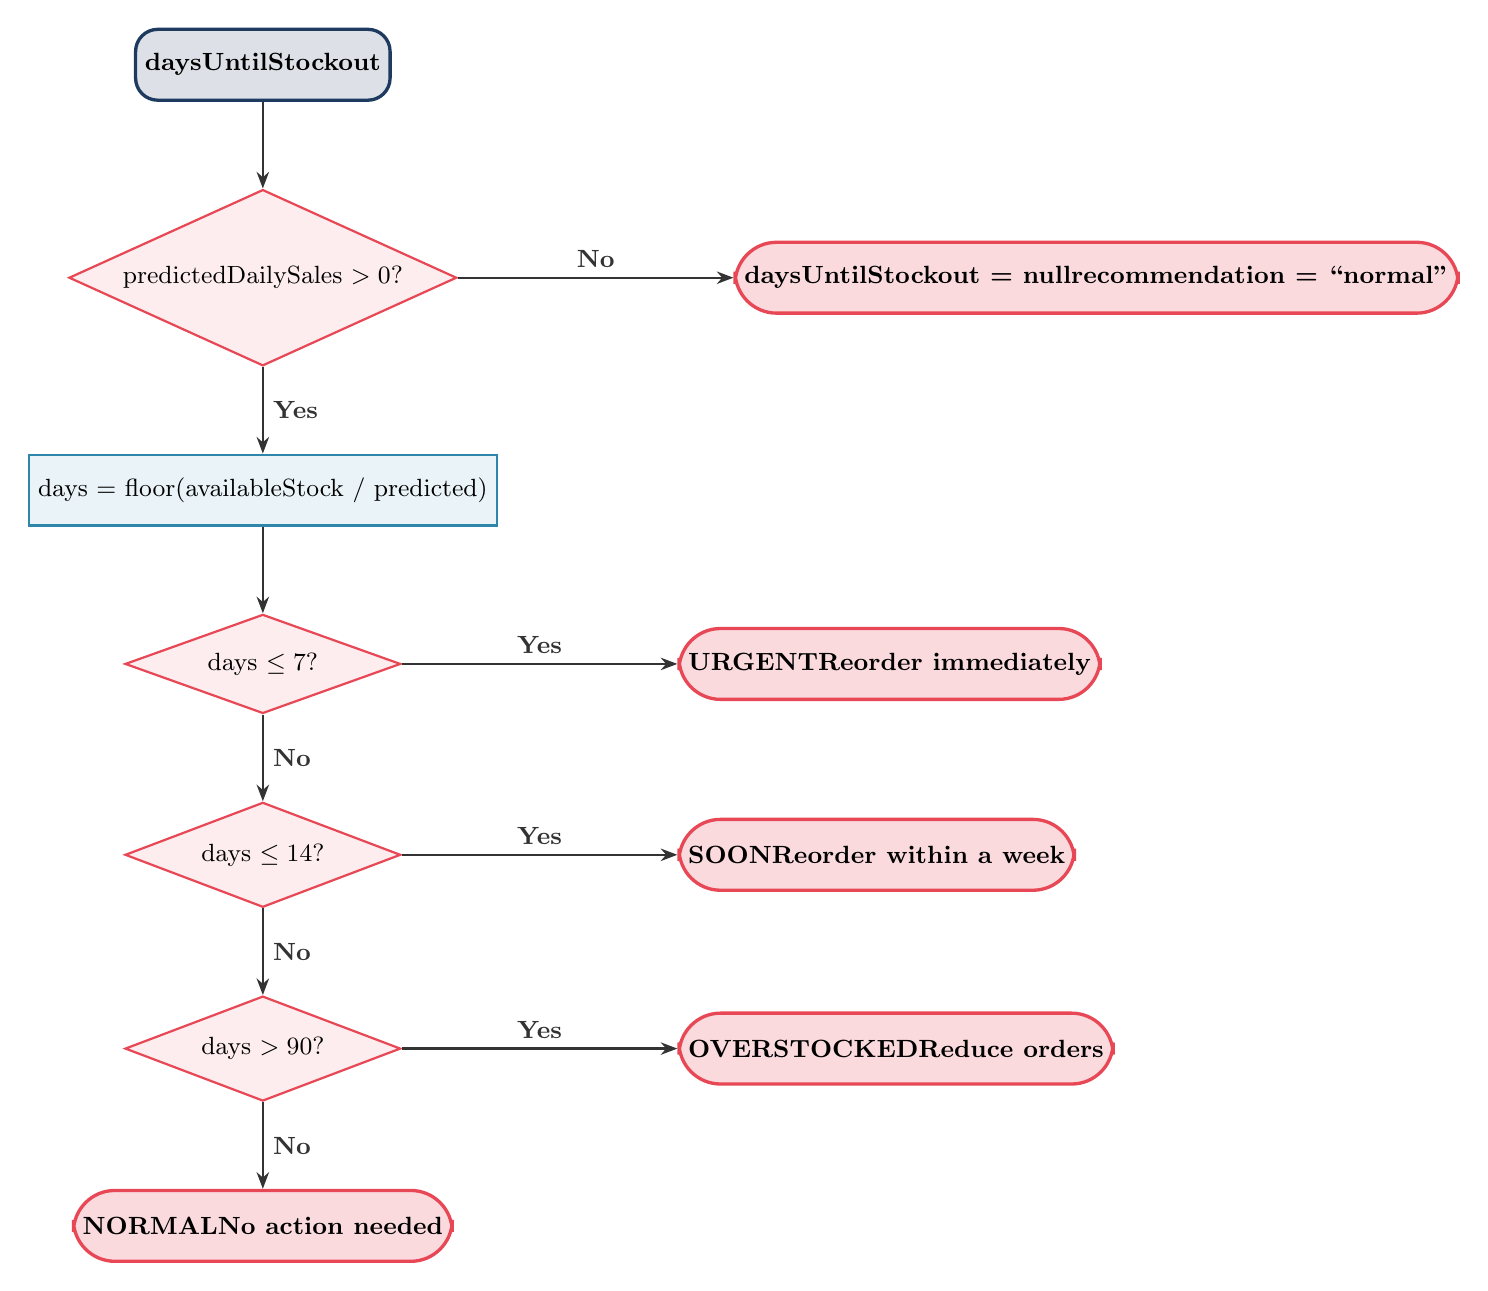
\begin{tikzpicture}[node distance=1.1cm]

  \node[startstop] (start) {daysUntilStockout};
  \node[decision, below=of start] (d1) {predictedDailySales $> 0$?};
  \node[terminal, right=3.5cm of d1] (null) {daysUntilStockout = null \\ recommendation = ``normal''};
  \node[process, below=of d1] (calc) {days = floor(availableStock / predicted)};
  \node[decision, below=of calc] (d2) {days $\leq 7$?};
  \node[terminal, right=3.5cm of d2] (urgent) {\textbf{URGENT} \\ Reorder immediately};
  \node[decision, below=of d2] (d3) {days $\leq 14$?};
  \node[terminal, right=3.5cm of d3] (soon) {\textbf{SOON} \\ Reorder within a week};
  \node[decision, below=of d3] (d4) {days $> 90$?};
  \node[terminal, right=3.5cm of d4] (over) {\textbf{OVERSTOCKED} \\ Reduce orders};
  \node[terminal, below=of d4] (normal) {\textbf{NORMAL} \\ No action needed};

  \draw[arrow] (start) -- (d1);
  \draw[arrow] (d1) -- node[no, above]{No} (null);
  \draw[arrow] (d1) -- node[yes, right]{Yes} (calc);
  \draw[arrow] (calc) -- (d2);
  \draw[arrow] (d2) -- node[yes, above]{Yes} (urgent);
  \draw[arrow] (d2) -- node[no, right]{No} (d3);
  \draw[arrow] (d3) -- node[yes, above]{Yes} (soon);
  \draw[arrow] (d3) -- node[no, right]{No} (d4);
  \draw[arrow] (d4) -- node[yes, above]{Yes} (over);
  \draw[arrow] (d4) -- node[no, right]{No} (normal);

\end{tikzpicture}
\caption{Reorder recommendation decision tree with boundary values}
\end{figure}

\section{Test Cases --- Demand Forecasting}

\begin{tcolorbox}[testbox, title={FORE-001 \hfill \ptwo}]
\textbf{Function:} \texttt{calculateMovingAverage} \\
\textbf{Scenario:} Window larger than data length \\
\textbf{Input:} \texttt{values = [10, 20, 30]}, \texttt{window = 5} \\
\textbf{Expected:} \texttt{[10, 15, 20]} (partial windows used for early elements) \\
\textbf{Coverage:} \texttt{Math.max(0, i - window + 1)} branch for early indices
\end{tcolorbox}

\begin{tcolorbox}[testbox, title={FORE-004 \hfill \pone}]
\textbf{Function:} \texttt{calculateStdDev} \\
\textbf{Scenario:} Empty array \\
\textbf{Input:} \texttt{values = []} \\
\textbf{Expected:} \texttt{0} (early return branch) \\
\textbf{Coverage:} Empty array branch
\end{tcolorbox}

\begin{tcolorbox}[criticalbox, title={FORE-005 \hfill \pone\ --- Zero Variance}]
\textbf{Function:} \texttt{calculateStdDev} \\
\textbf{Scenario:} All identical values (zero variance) \\
\textbf{Input:} \texttt{values = [5, 5, 5, 5, 5]} \\
\textbf{Expected:} \texttt{0} \\
\textbf{Note:} Critical for anomaly detection --- if stdDev = 0, detectAnomalies returns \texttt{[]} \\
\textbf{Coverage:} Zero variance case
\end{tcolorbox}

\begin{tcolorbox}[testbox, title={FORE-007 \hfill \pone}]
\textbf{Function:} \texttt{analyzeTrend} \\
\textbf{Scenario:} Less than 7 data points \\
\textbf{Input:} 6 days of data \\
\textbf{Expected:} \texttt{\{ trend: "stable", percentageChange: 0, periodDays: 6 \}} \\
\textbf{Coverage:} Branch A (insufficient data)
\end{tcolorbox}

\begin{tcolorbox}[testbox, title={FORE-008 \hfill \pone\ --- Boundary}]
\textbf{Function:} \texttt{analyzeTrend} \\
\textbf{Scenario:} Exactly 7 data points (boundary value) \\
\textbf{Input:} 7 days of data with clear upward trend \\
\textbf{Expected:} \texttt{trend = "increasing"} (NOT blocked by \texttt{< 7} check) \\
\textbf{Coverage:} Boundary value (exactly 7)
\end{tcolorbox}

\begin{tcolorbox}[criticalbox, title={FORE-012 \hfill \pone\ --- Division by Zero}]
\textbf{Function:} \texttt{analyzeTrend} \\
\textbf{Scenario:} All zero sales (\texttt{avgY = 0}) \\
\textbf{Input:} 8 days of \texttt{quantity = 0} \\
\textbf{Internal:} \texttt{avgY = 0} $\to$ \texttt{percentageChange = 0} (division by zero protection) \\
\textbf{Expected:} \texttt{trend = "stable"}, \texttt{percentageChange = 0} \\
\textbf{Coverage:} Division by zero protection
\end{tcolorbox}

\begin{tcolorbox}[criticalbox, title={FORE-018 \hfill \pone\ --- Zero Sales Stockout}]
\textbf{Function:} \texttt{generateProductForecast} \\
\textbf{Scenario:} Zero predicted daily sales (no sales history) \\
\textbf{Input:} \texttt{dailySales = []} \\
\textbf{Internal:} \texttt{predictedDailySales = 0} $\to$ division by zero protection \\
\textbf{Expected:} \texttt{daysUntilStockout = null} (not \texttt{Infinity} or \texttt{NaN}) \\
\textbf{Coverage:} Division by zero protection in daysUntilStockout
\end{tcolorbox}

\begin{tcolorbox}[testbox, title={FORE-019 \hfill \pone}]
\textbf{Function:} \texttt{generateProductForecast} \\
\textbf{Scenario:} Urgent reorder (\texttt{daysUntilStockout = 5}) \\
\textbf{Input:} \texttt{availableStock=50}, \texttt{predictedDailySales=10} $\to$ days = 5 \\
\textbf{Expected:} \texttt{reorderRecommendation = "urgent"} ($5 \leq 7$) \\
\textbf{Coverage:} Urgent branch
\end{tcolorbox}

\begin{tcolorbox}[testbox, title={FORE-020 \hfill \pone\ --- Boundary}]
\textbf{Function:} \texttt{generateProductForecast} \\
\textbf{Scenario:} \texttt{daysUntilStockout = 7} (exactly at lead days boundary) \\
\textbf{Input:} \texttt{availableStock=70}, \texttt{predictedDailySales=10} $\to$ days = 7 \\
\textbf{Expected:} \texttt{reorderRecommendation = "urgent"} ($7 \leq 7$) \\
\textbf{Coverage:} Boundary value for urgent
\end{tcolorbox}

\begin{tcolorbox}[testbox, title={FORE-022 \hfill \ptwo}]
\textbf{Function:} \texttt{generateProductForecast} \\
\textbf{Scenario:} Overstocked (\texttt{daysUntilStockout = 91}) \\
\textbf{Input:} \texttt{availableStock=910}, \texttt{predictedDailySales=10} $\to$ days = 91 \\
\textbf{Expected:} \texttt{reorderRecommendation = "overstocked"} ($91 > 90$) \\
\textbf{Coverage:} Overstocked branch
\end{tcolorbox}

\begin{tcolorbox}[testbox, title={FORE-023 \hfill \ptwo\ --- Boundary}]
\textbf{Function:} \texttt{generateProductForecast} \\
\textbf{Scenario:} \texttt{daysUntilStockout = 90} (NOT overstocked) \\
\textbf{Input:} \texttt{availableStock=900}, \texttt{predictedDailySales=10} $\to$ days = 90 \\
\textbf{Expected:} \texttt{reorderRecommendation = "normal"} ($90$ is NOT $> 90$) \\
\textbf{Coverage:} Boundary value for overstocked
\end{tcolorbox}


% ══════════════════════════════════════════════════════════════════════════════

\chapter{Module 5: Email Notification System}
% ══════════════════════════════════════════════════════════════════════════════

\textbf{Source File:} \texttt{lib/email/notifications.ts}

\section{isLowStock \& isOutOfStock Logic}

\begin{tcolorbox}[infobox, title={Stock Alert Thresholds}]
\begin{itemize}
  \item \texttt{LOW\_STOCK\_THRESHOLD = 20}
  \item \texttt{isLowStock(qty, threshold=20):} \texttt{qty > 0 \&\& qty <= threshold}
  \item \texttt{isOutOfStock(qty):} \texttt{qty === 0} (strict equality)
\end{itemize}
\end{tcolorbox}

\subsection{isLowStock Truth Table}

\begin{center}
\begin{tabular}{rrlc}
  \toprule
  \textbf{quantity} & \textbf{threshold} & \textbf{Evaluation} & \textbf{Result} \\
  \midrule
  0  & 20 & $0 > 0$ is FALSE (short-circuit) & \texttt{false} \\
  1  & 20 & $1 > 0$ AND $1 \leq 20$          & \texttt{true} \\
  20 & 20 & $20 > 0$ AND $20 \leq 20$        & \texttt{true} \\
  21 & 20 & $21 > 0$ AND $21 \leq 20$ = FALSE & \texttt{false} \\
  $-1$ & 20 & $-1 > 0$ is FALSE (short-circuit) & \texttt{false} \\
  \bottomrule
\end{tabular}
\end{center}

\subsection{sendLowStockAlert Control Flow}

\begin{figure}[h!]
\centering
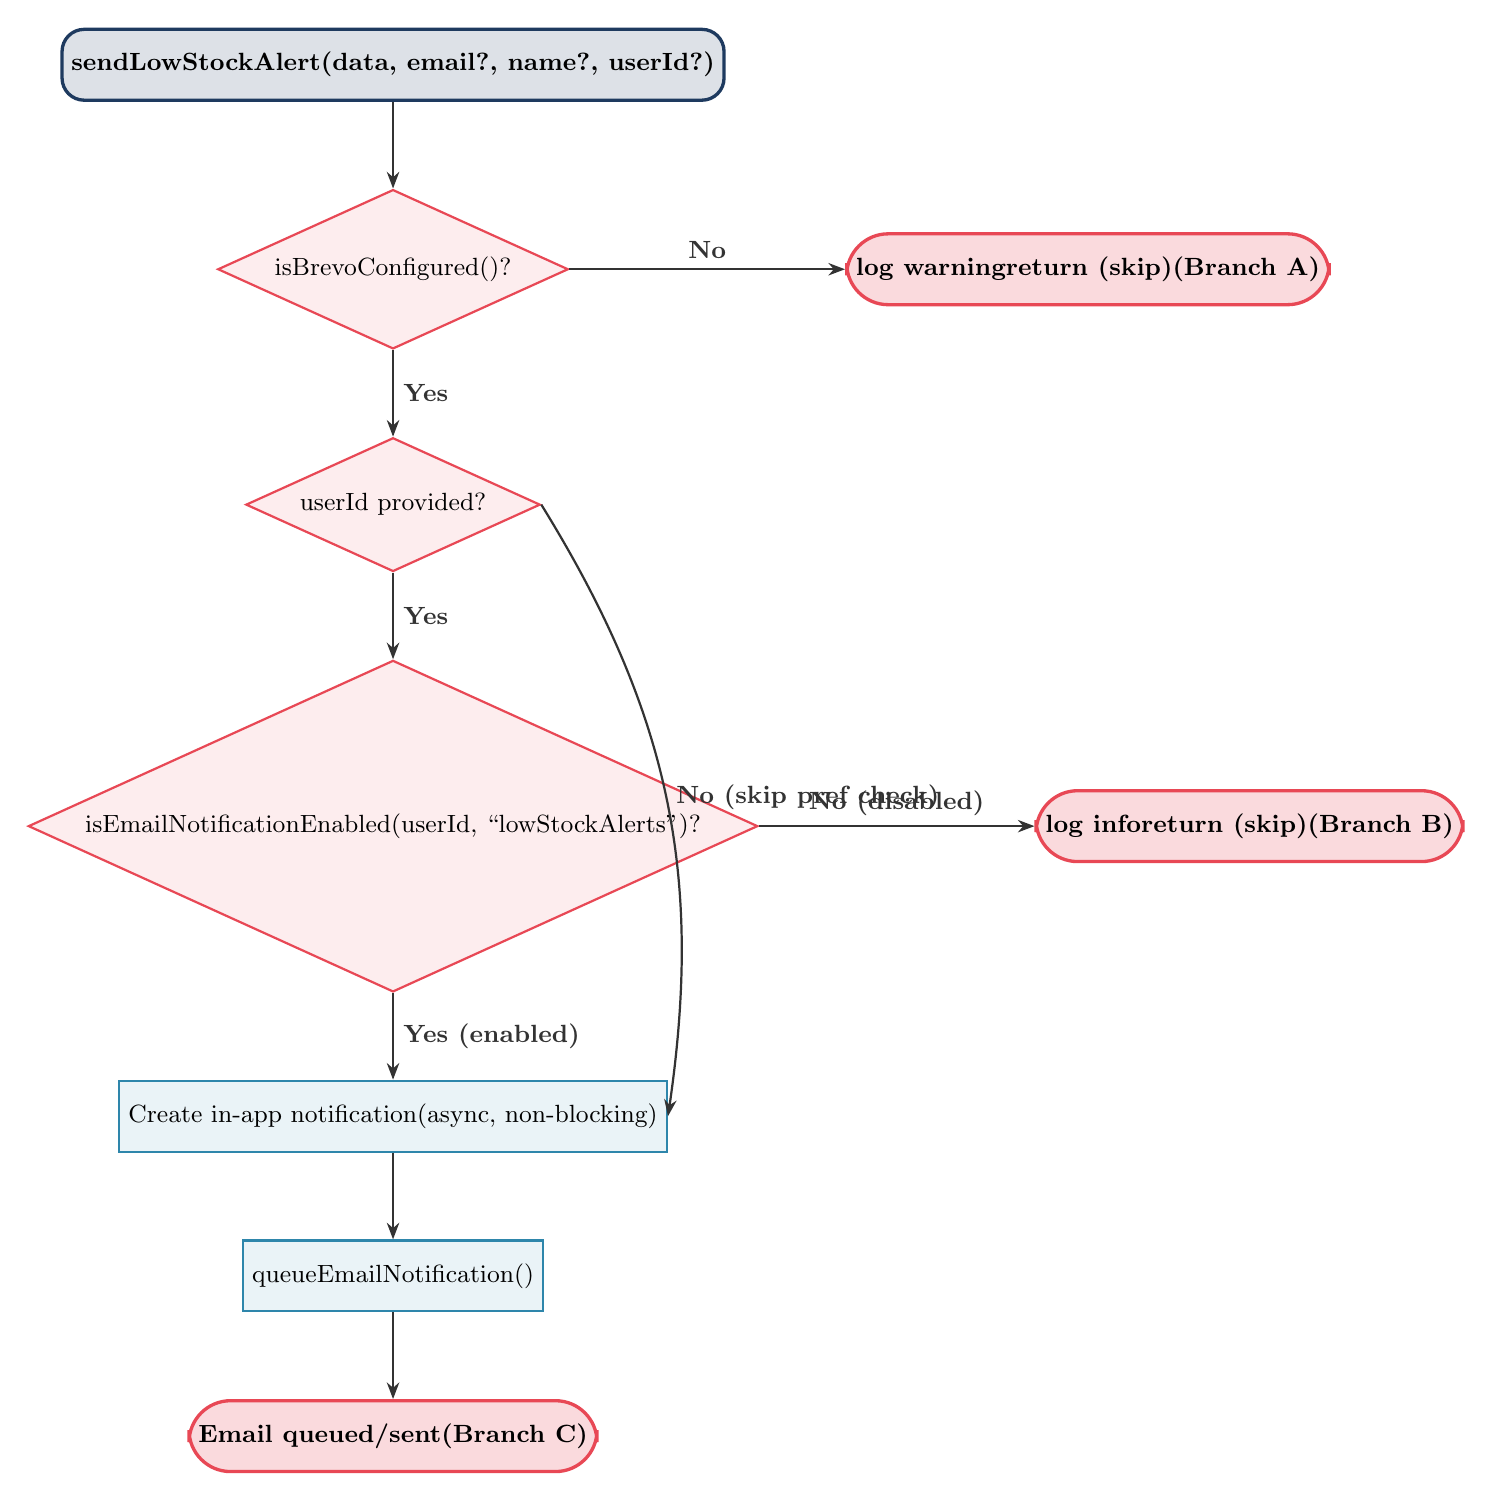
\begin{tikzpicture}[node distance=1.1cm]

  \node[startstop] (start) {sendLowStockAlert(data, email?, name?, userId?)};
  \node[decision, below=of start] (d1) {isBrevoConfigured()?};
  \node[terminal, right=3.5cm of d1] (rA) {log warning \\ return (skip) \\ \small(Branch A)};
  \node[decision, below=of d1] (d2) {userId provided?};
  \node[decision, below=of d2] (d3) {isEmailNotificationEnabled \\ (userId, ``lowStockAlerts'')?};
  \node[terminal, right=3.5cm of d3] (rB) {log info \\ return (skip) \\ \small(Branch B)};
  \node[process, below=of d3] (inapp) {Create in-app notification \\ (async, non-blocking)};
  \node[process, below=of inapp] (queue) {queueEmailNotification()};
  \node[terminal, below=of queue] (rC) {Email queued/sent \\ \small(Branch C)};

  \draw[arrow] (start) -- (d1);
  \draw[arrow] (d1) -- node[no, above]{No} (rA);
  \draw[arrow] (d1) -- node[yes, right]{Yes} (d2);
  \draw[arrow] (d2.east) to[bend left=20] node[no, right]{No (skip pref check)} (inapp.east);
  \draw[arrow] (d2) -- node[yes, right]{Yes} (d3);
  \draw[arrow] (d3) -- node[no, above]{No (disabled)} (rB);
  \draw[arrow] (d3) -- node[yes, right]{Yes (enabled)} (inapp);
  \draw[arrow] (inapp) -- (queue);
  \draw[arrow] (queue) -- (rC);

\end{tikzpicture}
\caption{sendLowStockAlert control flow with all branches}
\end{figure}

\section{Test Cases --- Email Notifications}

\begin{tcolorbox}[criticalbox, title={EMAIL-001 \hfill \pone\ --- Out of Stock Not Low Stock}]
\textbf{Function:} \texttt{isLowStock} \\
\textbf{Scenario:} Quantity is 0 (out of stock, not low stock) \\
\textbf{Input:} \texttt{quantity = 0}, \texttt{threshold = 20} \\
\textbf{Internal:} $0 > 0$ is \texttt{FALSE} $\to$ short-circuit $\to$ \texttt{return false} \\
\textbf{Expected:} \texttt{false} \\
\textbf{Coverage:} First condition false (AND short-circuit)
\end{tcolorbox}

\begin{tcolorbox}[testbox, title={EMAIL-002 \hfill \pone\ --- At Threshold Boundary}]
\textbf{Function:} \texttt{isLowStock} \\
\textbf{Scenario:} Quantity exactly at threshold \\
\textbf{Input:} \texttt{quantity = 20}, \texttt{threshold = 20} \\
\textbf{Internal:} $20 > 0$ AND $20 \leq 20$ $\to$ \texttt{true} \\
\textbf{Expected:} \texttt{true} \\
\textbf{Coverage:} Boundary value (at threshold)
\end{tcolorbox}

\begin{tcolorbox}[testbox, title={EMAIL-003 \hfill \pone\ --- Above Threshold}]
\textbf{Function:} \texttt{isLowStock} \\
\textbf{Scenario:} Quantity one above threshold \\
\textbf{Input:} \texttt{quantity = 21}, \texttt{threshold = 20} \\
\textbf{Internal:} $21 > 0$ AND $21 \leq 20$ $\to$ \texttt{false} \\
\textbf{Expected:} \texttt{false} \\
\textbf{Coverage:} Boundary value + 1
\end{tcolorbox}

\begin{tcolorbox}[testbox, title={EMAIL-007 \hfill \pone}]
\textbf{Function:} \texttt{isOutOfStock} \\
\textbf{Scenario:} Quantity is exactly 0 \\
\textbf{Input:} \texttt{quantity = 0} \\
\textbf{Internal:} \texttt{0 === 0} $\to$ \texttt{true} \\
\textbf{Expected:} \texttt{true} \\
\textbf{Coverage:} Exact zero match
\end{tcolorbox}

\begin{tcolorbox}[testbox, title={EMAIL-009 \hfill \ptwo}]
\textbf{Function:} \texttt{isOutOfStock} \\
\textbf{Scenario:} Negative quantity (corrupted data) \\
\textbf{Input:} \texttt{quantity = -1} \\
\textbf{Internal:} \texttt{-1 === 0} is \texttt{false} (strict equality) \\
\textbf{Expected:} \texttt{false} \\
\textbf{Coverage:} Strict equality check
\end{tcolorbox}

\begin{tcolorbox}[testbox, title={EMAIL-010 \hfill \pone}]
\textbf{Function:} \texttt{sendLowStockAlert} \\
\textbf{Scenario:} Brevo not configured \\
\textbf{Mock:} \texttt{isBrevoConfigured()} returns \texttt{false} \\
\textbf{Expected:} Function returns early, no email sent, warning logged \\
\textbf{Coverage:} Branch A
\end{tcolorbox}

\begin{tcolorbox}[testbox, title={EMAIL-011 \hfill \ptwo}]
\textbf{Function:} \texttt{sendLowStockAlert} \\
\textbf{Scenario:} User has disabled low stock alerts \\
\textbf{Mock:} \texttt{isBrevoConfigured()} = \texttt{true}; \texttt{isEmailNotificationEnabled} = \texttt{false} \\
\textbf{Expected:} Function returns early, no email sent, info logged \\
\textbf{Coverage:} Branch B
\end{tcolorbox}

% ══════════════════════════════════════════════════════════════════════════════

\chapter{Module 6: Rate Limiting \& Caching}
% ══════════════════════════════════════════════════════════════════════════════

\textbf{Source File:} \texttt{lib/api/rate-limit.ts}

\section{Rate Limit Configurations}

\begin{center}
\begin{tabular}{lccp{6cm}}
  \toprule
  \textbf{Config} & \textbf{Limit} & \textbf{Window} & \textbf{Identifier} \\
  \midrule
  \texttt{standard} & 600 req & 60 sec & User ID (header) or IP \\
  \texttt{strict}   & 10 req  & 60 sec & User ID (header) or IP \\
  \texttt{auth}     & 5 req   & 60 sec & \textbf{Always IP} (brute-force protection) \\
  \bottomrule
\end{tabular}
\end{center}

\subsection{Identifier Resolution Flowchart}

\begin{figure}[h!]
\centering
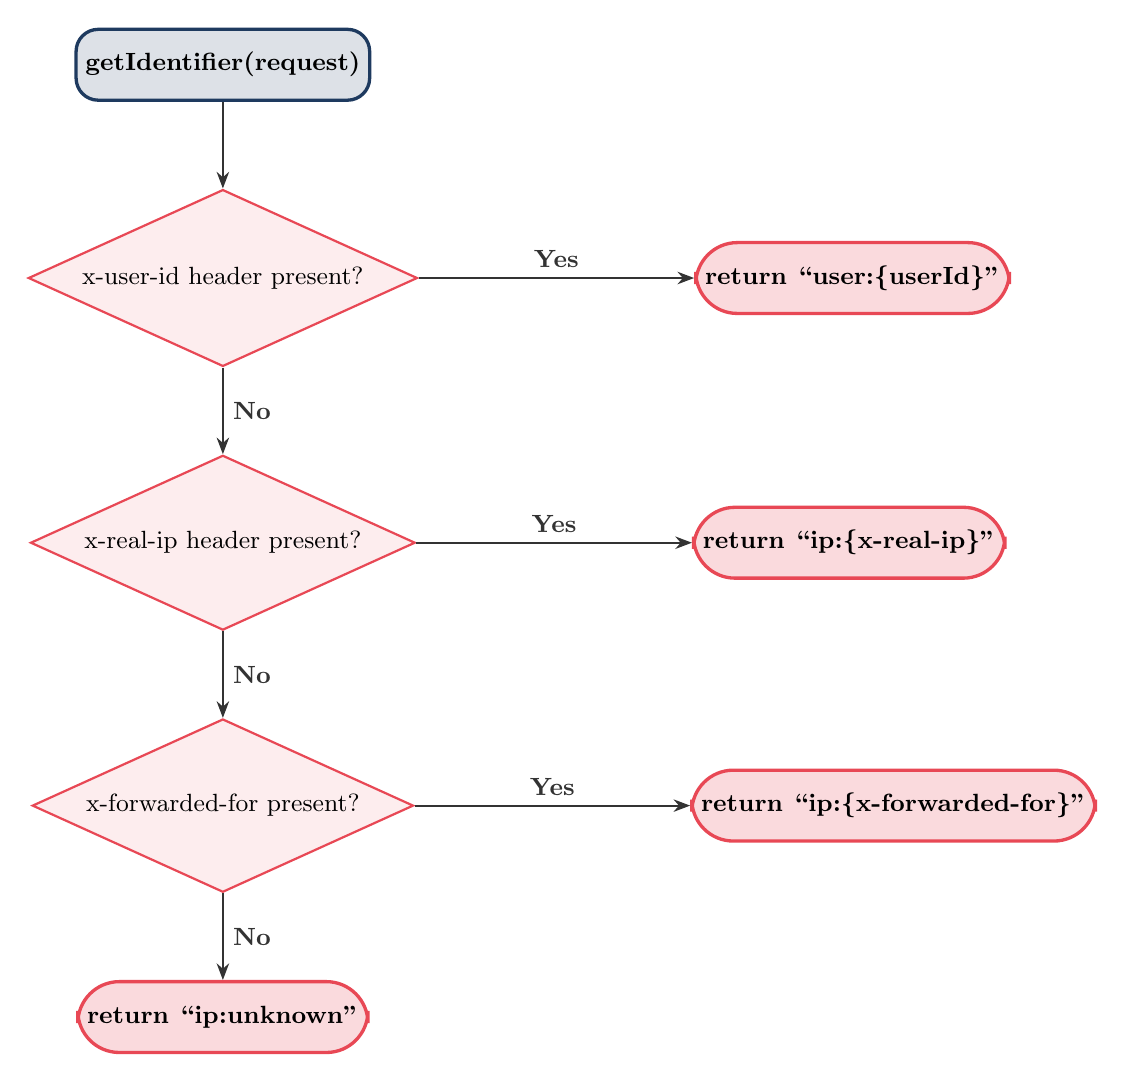
\begin{tikzpicture}[node distance=1.1cm]

  \node[startstop] (start) {getIdentifier(request)};
  \node[decision, below=of start] (d1) {x-user-id header present?};
  \node[terminal, right=3.5cm of d1] (uid) {return ``user:\{userId\}''};
  \node[decision, below=of d1] (d2) {x-real-ip header present?};
  \node[terminal, right=3.5cm of d2] (rip) {return ``ip:\{x-real-ip\}''};
  \node[decision, below=of d2] (d3) {x-forwarded-for present?};
  \node[terminal, right=3.5cm of d3] (fwd) {return ``ip:\{x-forwarded-for\}''};
  \node[terminal, below=of d3] (unk) {return ``ip:unknown''};

  \draw[arrow] (start) -- (d1);
  \draw[arrow] (d1) -- node[yes, above]{Yes} (uid);
  \draw[arrow] (d1) -- node[no, right]{No} (d2);
  \draw[arrow] (d2) -- node[yes, above]{Yes} (rip);
  \draw[arrow] (d2) -- node[no, right]{No} (d3);
  \draw[arrow] (d3) -- node[yes, above]{Yes} (fwd);
  \draw[arrow] (d3) -- node[no, right]{No} (unk);

\end{tikzpicture}
\caption{Rate limit identifier resolution (standard/strict configs)}
\end{figure}

\section{Test Cases --- Rate Limiting}

\begin{tcolorbox}[criticalbox, title={RATE-005 \hfill \pone\ --- Auth Always Uses IP}]
\textbf{Config:} \texttt{defaultRateLimits.auth} \\
\textbf{Scenario:} Auth endpoint always uses IP even if user ID header present \\
\textbf{Input:} Request with \texttt{x-user-id = "user123"} AND \texttt{x-real-ip = "1.2.3.4"} \\
\textbf{Expected:} \texttt{"ip:1.2.3.4"} (NOT \texttt{"user:user123"}) \\
\textbf{Coverage:} Auth always-IP security requirement
\end{tcolorbox}

\begin{tcolorbox}[testbox, title={RATE-007 \hfill \pone}]
\textbf{Function:} \texttt{withRateLimit} \\
\textbf{Scenario:} Rate limit exceeded \\
\textbf{Mock:} \texttt{checkRateLimit} returns \texttt{\{ limited: true, retryAfter: 30 \}} \\
\textbf{Expected:} Returns \texttt{NextResponse} with status \textbf{429} and \texttt{Retry-After} header \\
\textbf{Coverage:} Rate limited branch
\end{tcolorbox}

% ══════════════════════════════════════════════════════════════════════════════

\chapter{Module 7: Input Validation (Zod Schemas)}
% ══════════════════════════════════════════════════════════════════════════════

\section{Validation Behaviour}

\begin{tcolorbox}[infobox, title={Zod Schema Behaviour}]
When \texttt{schema.parse(data)} is called:
\begin{itemize}
  \item \textbf{Valid data:} Returns typed, parsed data object.
  \item \textbf{Invalid data:} Throws \texttt{ZodError} with field-level error messages.
\end{itemize}
The login route catches \texttt{ZodError} and returns HTTP 400.
\end{tcolorbox}

\section{Test Cases --- Input Validation}

\begin{tcolorbox}[testbox, title={VAL-002 \hfill \pone}]
\textbf{Schema:} \texttt{loginSchema} \\
\textbf{Scenario:} Invalid email format \\
\textbf{Input:} \texttt{\{ email: "not-an-email", password: "pass123" \}} \\
\textbf{Expected:} \texttt{ZodError} thrown, error on \texttt{"email"} field \\
\textbf{Coverage:} Email format validation
\end{tcolorbox}

\begin{tcolorbox}[criticalbox, title={VAL-006 \hfill \pone\ --- Zero Quantity}]
\textbf{Schema:} \texttt{createOrderSchema} \\
\textbf{Scenario:} Item with \texttt{quantity = 0} \\
\textbf{Input:} \texttt{\{ items: [\{ productId: "abc", quantity: 0 \}] \}} \\
\textbf{Expected:} \texttt{ZodError} (if \texttt{min(1)} enforced on quantity) \\
\textbf{Coverage:} Zero quantity validation
\end{tcolorbox}

\begin{tcolorbox}[criticalbox, title={VAL-012 \hfill \pone\ --- Injection Attempt}]
\textbf{Scenario:} NoSQL injection attempt in email field \\
\textbf{Input:} \texttt{\{ email: "\$where: function() \{ return true; \}" \}} \\
\textbf{Expected:} \texttt{ZodError} (invalid email format) or safely stored as string \\
\textbf{Note:} MongoDB is not SQL-injectable, but Zod should reject invalid emails \\
\textbf{Coverage:} Injection attempt handling
\end{tcolorbox}

\begin{tcolorbox}[criticalbox, title={VAL-013 \hfill \pone\ --- XSS Attempt}]
\textbf{Scenario:} XSS attempt in notes field \\
\textbf{Input:} \texttt{\{ notes: "<script>alert('xss')</script>" \}} \\
\textbf{Expected:} Stored as plain string (no execution), or sanitized \\
\textbf{Coverage:} XSS in text fields
\end{tcolorbox}


% ══════════════════════════════════════════════════════════════════════════════

\chapter{Module 8: Role-Based Access Control (RBAC)}
% ══════════════════════════════════════════════════════════════════════════════

\section{RBAC Decision Flowchart}

\begin{figure}[h!]
\centering
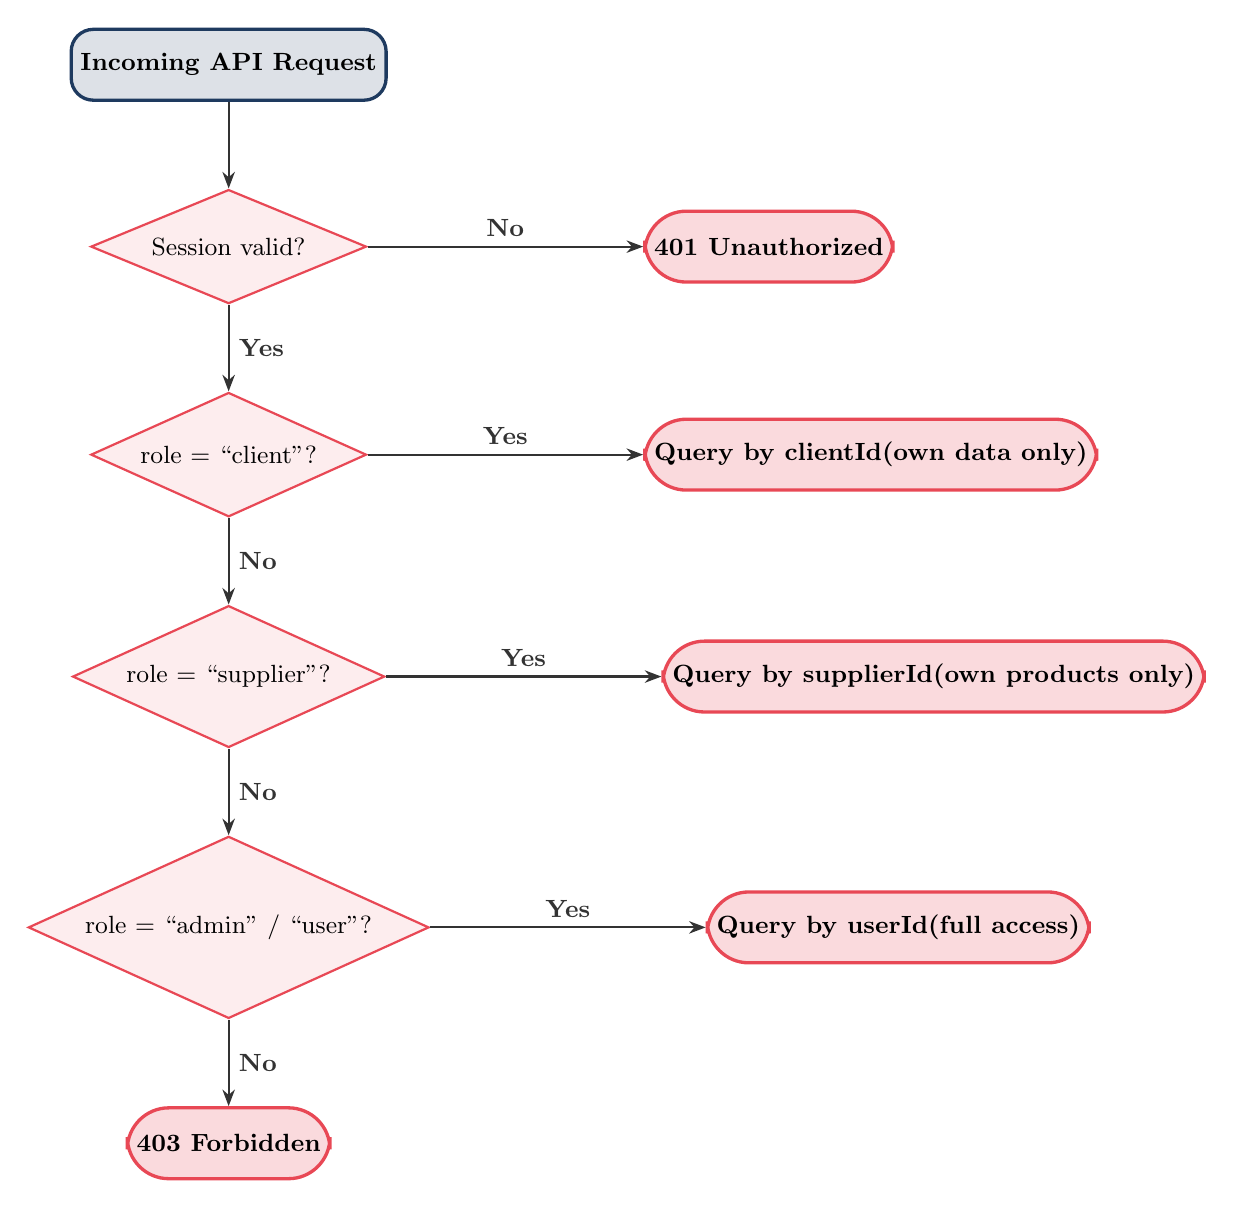
\begin{tikzpicture}[node distance=1.1cm]

  \node[startstop] (start) {Incoming API Request};
  \node[decision, below=of start] (d1) {Session valid?};
  \node[terminal, right=3.5cm of d1] (r401) {401 Unauthorized};
  \node[decision, below=of d1] (d2) {role = ``client''?};
  \node[terminal, right=3.5cm of d2] (client) {Query by clientId \\ (own data only)};
  \node[decision, below=of d2] (d3) {role = ``supplier''?};
  \node[terminal, right=3.5cm of d3] (supplier) {Query by supplierId \\ (own products only)};
  \node[decision, below=of d3] (d4) {role = ``admin'' / ``user''?};
  \node[terminal, right=3.5cm of d4] (admin) {Query by userId \\ (full access)};
  \node[terminal, below=of d4] (r403) {403 Forbidden};

  \draw[arrow] (start) -- (d1);
  \draw[arrow] (d1) -- node[no, above]{No} (r401);
  \draw[arrow] (d1) -- node[yes, right]{Yes} (d2);
  \draw[arrow] (d2) -- node[yes, above]{Yes} (client);
  \draw[arrow] (d2) -- node[no, right]{No} (d3);
  \draw[arrow] (d3) -- node[yes, above]{Yes} (supplier);
  \draw[arrow] (d3) -- node[no, right]{No} (d4);
  \draw[arrow] (d4) -- node[yes, above]{Yes} (admin);
  \draw[arrow] (d4) -- node[no, right]{No} (r403);

\end{tikzpicture}
\caption{RBAC decision flow for API routes}
\end{figure}

\section{Test Cases --- RBAC}

\begin{tcolorbox}[criticalbox, title={RBAC-008 \hfill \pone\ --- Unauthenticated}]
\textbf{Scenario:} Unauthenticated request to any protected route \\
\textbf{Mock:} \texttt{getSessionFromRequest} returns \texttt{null} \\
\textbf{Expected:} \textbf{401 Unauthorized} response \\
\textbf{Coverage:} Auth guard (all routes)
\end{tcolorbox}

\begin{tcolorbox}[criticalbox, title={RBAC-010 \hfill \pone\ --- Data Isolation}]
\textbf{Scenario:} Supplier tries to access another supplier's products \\
\textbf{Mock:} \texttt{session.role = "supplier"}, \texttt{supplierId = "supplierA"} \\
\textbf{Expected:} Only products with \texttt{supplierId = "supplierA"} returned \\
\textbf{Coverage:} Data isolation between suppliers
\end{tcolorbox}

\begin{tcolorbox}[criticalbox, title={RBAC-011 \hfill \pone\ --- Horizontal Privilege Escalation}]
\textbf{Scenario:} User tries to access another user's orders \\
\textbf{Mock:} \texttt{session.id = "userA"}, request attempts to get orders for \texttt{"userB"} \\
\textbf{Expected:} Only userA's orders returned (userId from session, not request body) \\
\textbf{Coverage:} Horizontal privilege escalation prevention
\end{tcolorbox}

% ══════════════════════════════════════════════════════════════════════════════

\chapter{Module 9: Data Integrity \& Database Layer}
% ══════════════════════════════════════════════════════════════════════════════

\section{Unique Constraints}

\begin{center}
\begin{tabular}{lll}
  \toprule
  \textbf{Model} & \textbf{Field} & \textbf{Constraint} \\
  \midrule
  \texttt{User}    & \texttt{email}         & Globally unique \\
  \texttt{Product} & \texttt{sku}           & Globally unique \\
  \texttt{Order}   & \texttt{orderNumber}   & Globally unique \\
  \texttt{Invoice} & \texttt{invoiceNumber} & Globally unique \\
  \texttt{Invoice} & \texttt{orderId}       & Unique (one invoice per order) \\
  \bottomrule
\end{tabular}
\end{center}

\section{Cascade Relationships}

\begin{center}
\begin{tabular}{lll}
  \toprule
  \textbf{Parent} & \textbf{Child} & \textbf{On Delete} \\
  \midrule
  \texttt{Order}         & \texttt{Invoice}   & Cascade (invoice deleted) \\
  \texttt{Order}         & \texttt{OrderItem} & Cascade (items deleted) \\
  \texttt{User}          & \texttt{Notification} & Cascade \\
  \texttt{SupportTicket} & \texttt{SupportTicketReply} & Cascade \\
  \bottomrule
\end{tabular}
\end{center}

\section{Test Cases --- Data Integrity}

\begin{tcolorbox}[criticalbox, title={DB-004 \hfill \pone\ --- Cascade Delete}]
\textbf{Scenario:} Deleting an order removes its invoice \\
\textbf{Steps:} (1) Create order \quad (2) Create invoice for that order \quad (3) Delete the order \\
\textbf{Expected:} Invoice is also deleted (cascade) \\
\textbf{Coverage:} \texttt{onDelete: Cascade} relationship
\end{tcolorbox}

\begin{tcolorbox}[criticalbox, title={DB-007 \hfill \pone\ --- Atomicity Gap}]
\textbf{Scenario:} \texttt{prisma.product.update} fails after \texttt{order.create} succeeds \\
\textbf{Expected:} Order exists but stock not reserved (partial state) \\
\textbf{Note:} \textbf{Known issue} --- order creation is not wrapped in a database transaction. \\
This is a documented architectural risk. \\
\textbf{Coverage:} Transaction atomicity gap
\end{tcolorbox}

\begin{tcolorbox}[testbox, title={DB-008 \hfill \ptwo}]
\textbf{Scenario:} Audit log failure does not break main operation \\
\textbf{Mock:} \texttt{createAuditLog} throws an error \\
\textbf{Expected:} Main operation (order create, etc.) still succeeds \\
\textbf{Coverage:} Audit log error isolation (fire-and-forget)
\end{tcolorbox}

% ══════════════════════════════════════════════════════════════════════════════

\chapter{Module 10: Stripe Payment \& Webhook Handling}
% ══════════════════════════════════════════════════════════════════════════════

\section{Webhook Security Flow}

\begin{figure}[h!]
\centering
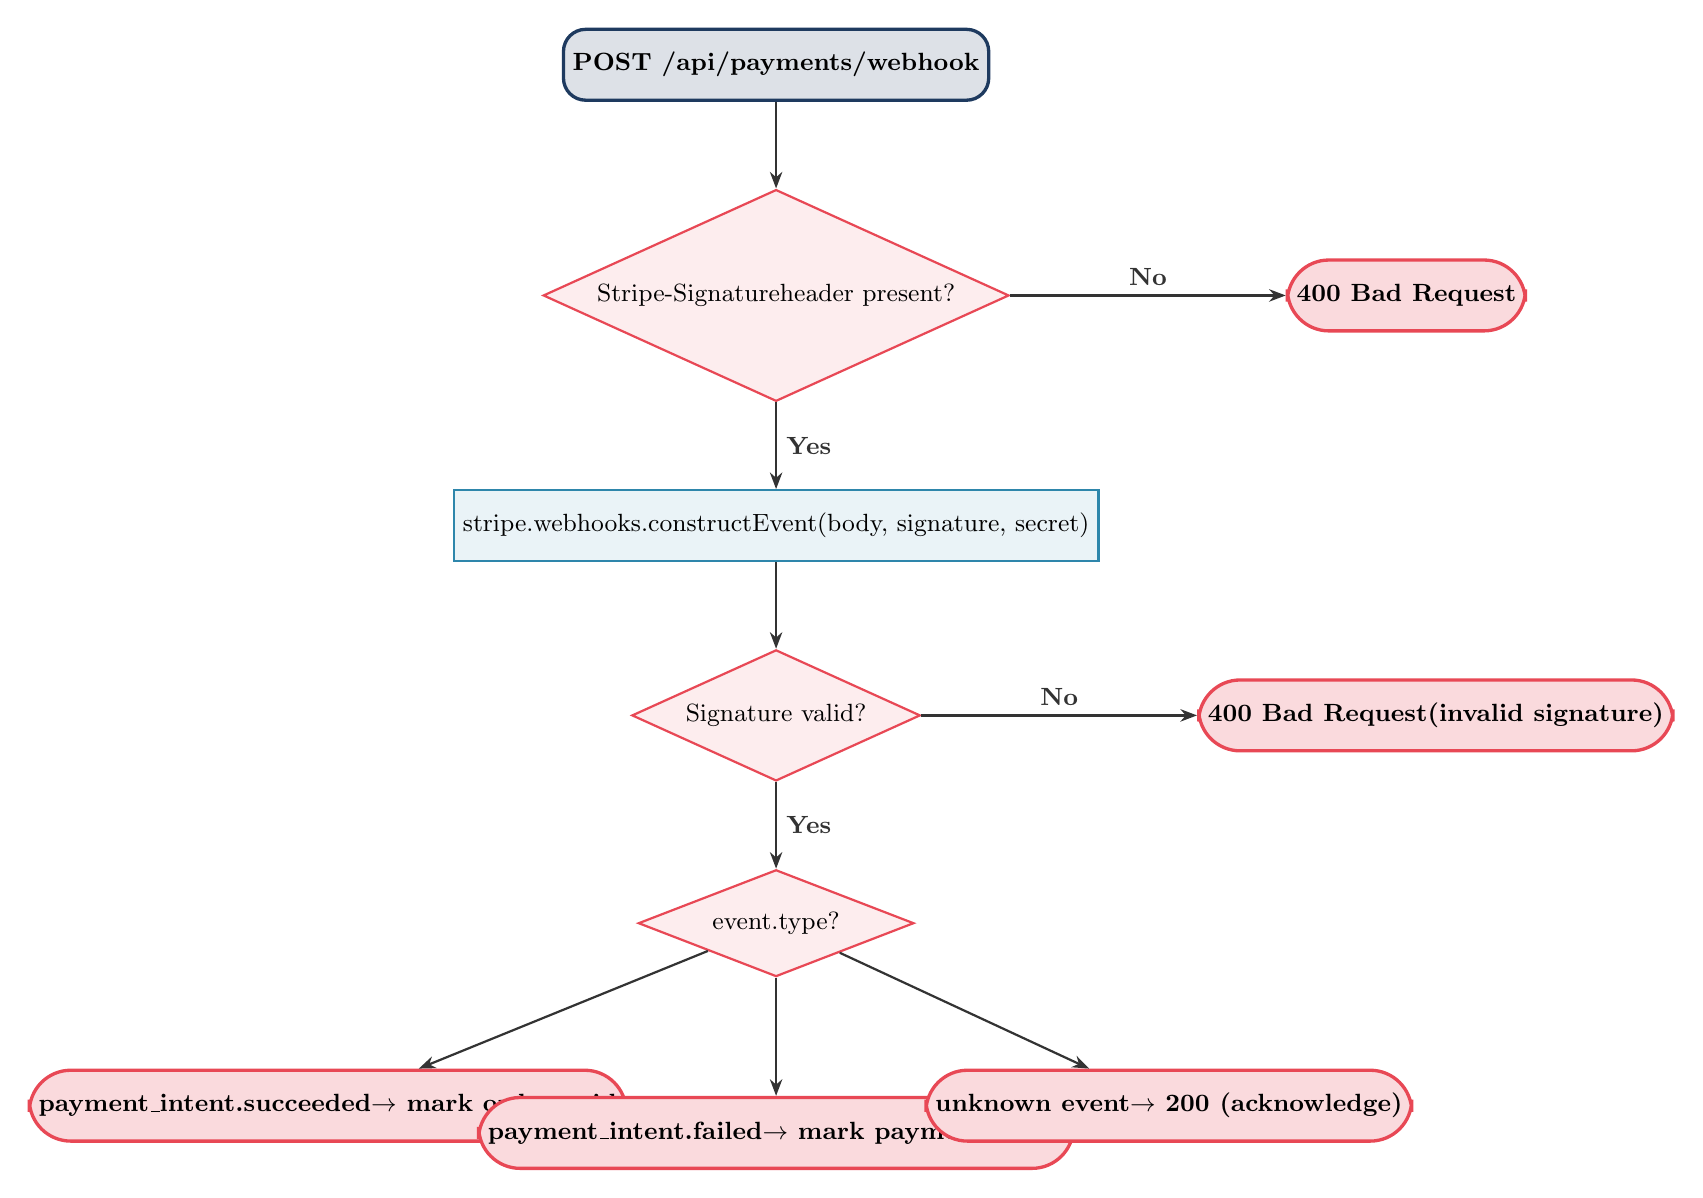
\begin{tikzpicture}[node distance=1.1cm]

  \node[startstop] (start) {POST /api/payments/webhook};
  \node[decision, below=of start] (d1) {Stripe-Signature \\ header present?};
  \node[terminal, right=3.5cm of d1] (r400a) {400 Bad Request};
  \node[process, below=of d1] (verify) {stripe.webhooks.constructEvent \\ (body, signature, secret)};
  \node[decision, below=of verify] (d2) {Signature valid?};
  \node[terminal, right=3.5cm of d2] (r400b) {400 Bad Request \\ (invalid signature)};
  \node[decision, below=of d2] (d3) {event.type?};
  \node[terminal, below left=1.5cm and 1cm of d3] (paid) {payment\_intent.succeeded \\ $\to$ mark order paid};
  \node[terminal, below=1.5cm of d3] (failed) {payment\_intent.failed \\ $\to$ mark payment failed};
  \node[terminal, below right=1.5cm and 1cm of d3] (other) {unknown event \\ $\to$ 200 (acknowledge)};

  \draw[arrow] (start) -- (d1);
  \draw[arrow] (d1) -- node[no, above]{No} (r400a);
  \draw[arrow] (d1) -- node[yes, right]{Yes} (verify);
  \draw[arrow] (verify) -- (d2);
  \draw[arrow] (d2) -- node[no, above]{No} (r400b);
  \draw[arrow] (d2) -- node[yes, right]{Yes} (d3);
  \draw[arrow] (d3) -- (paid);
  \draw[arrow] (d3) -- (failed);
  \draw[arrow] (d3) -- (other);

\end{tikzpicture}
\caption{Stripe webhook security and event handling flow}
\end{figure}

\section{Test Cases --- Stripe Payments}

\begin{tcolorbox}[criticalbox, title={PAY-001 \hfill \pone\ --- Invalid Signature}]
\textbf{Scenario:} Webhook with invalid signature \\
\textbf{Input:} Valid body but wrong \texttt{Stripe-Signature} header \\
\textbf{Expected:} \texttt{stripe.webhooks.constructEvent} throws $\to$ \textbf{400} response \\
\textbf{Coverage:} Signature verification failure branch
\end{tcolorbox}

\begin{tcolorbox}[criticalbox, title={PAY-002 \hfill \pone\ --- Missing Signature}]
\textbf{Scenario:} Webhook with no \texttt{Stripe-Signature} header \\
\textbf{Expected:} \textbf{400} response (cannot verify) \\
\textbf{Coverage:} Missing signature branch
\end{tcolorbox}

\begin{tcolorbox}[testbox, title={PAY-005 \hfill \ptwo}]
\textbf{Scenario:} Unknown webhook event type \\
\textbf{Mock:} \texttt{event.type = "some.unknown.event"} \\
\textbf{Expected:} Event ignored gracefully, \textbf{200} response (acknowledge receipt) \\
\textbf{Coverage:} Unknown event type branch
\end{tcolorbox}


% ══════════════════════════════════════════════════════════════════════════════

\chapter{Complete Test Case Matrix}
% ══════════════════════════════════════════════════════════════════════════════

\section{Authentication Tests}

\begin{longtable}{p{2cm}p{3.5cm}p{5cm}p{1.5cm}c}
  \toprule
  \textbf{Test ID} & \textbf{Function} & \textbf{Scenario} & \textbf{Coverage} & \textbf{Pri.} \\
  \midrule
  \endhead
  \testid{AUTH-001} & verifyToken & Empty string token & Branch A & \pone \\
  \testid{AUTH-002} & verifyToken & String ``null'' token & Branch A & \pone \\
  \testid{AUTH-003} & verifyToken & String ``undefined'' token & Branch A & \pone \\
  \testid{AUTH-004} & verifyToken & Valid JWT & Branch E & \pone \\
  \testid{AUTH-005} & verifyToken & Expired JWT & Exception & \pone \\
  \testid{AUTH-006} & verifyToken & Wrong secret & Security & \pone \\
  \testid{AUTH-007} & verifyToken & Malformed token & Exception & \pone \\
  \testid{AUTH-008} & generateToken & Payload integrity & Statement & \pone \\
  \testid{AUTH-009} & hashPassword + compare & Round-trip hash & Statement & \pone \\
  \testid{AUTH-010} & comparePassword & Wrong password & Branch & \pone \\
  \testid{AUTH-011} & POST /login & Missing email & Validation & \pone \\
  \testid{AUTH-012} & POST /login & User not found & Branch & \pone \\
  \testid{AUTH-013} & POST /login & Corrupted user data & Branch & \ptwo \\
  \testid{AUTH-014} & POST /login & Correct credentials & Statement & \pone \\
  \testid{AUTH-015} & getSession & No cookie & Branch & \pone \\
  \testid{AUTH-016} & getSession & Deleted user & Branch & \ptwo \\
  \bottomrule
\end{longtable}

\section{Order Management Tests}

\begin{longtable}{p{2cm}p{3.5cm}p{5cm}p{1.5cm}c}
  \toprule
  \textbf{Test ID} & \textbf{Function} & \textbf{Scenario} & \textbf{Coverage} & \textbf{Pri.} \\
  \midrule
  \endhead
  \testid{ORD-001} & generateOrderNumber & First order of day & Statement & \ptwo \\
  \testid{ORD-002} & generateOrderNumber & 9999 orders today & Boundary & \pthree \\
  \testid{ORD-003} & createOrder & Product not found & Branch & \pone \\
  \testid{ORD-004} & createOrder & Insufficient stock & Branch & \pone \\
  \testid{ORD-005} & createOrder & Exact stock match & Boundary & \pone \\
  \testid{ORD-006} & createOrder & Boundary + 1 & Boundary & \pone \\
  \testid{ORD-007} & createOrder & Null reservedQty & Branch & \ptwo \\
  \testid{ORD-008} & createOrder & Partial failure & Atomicity & \pone \\
  \testid{ORD-009} & createOrder & Total calculation & Statement & \pone \\
  \testid{ORD-010} & createOrder & Zero tax/shipping & Branch & \ptwo \\
  \testid{ORD-011} & createOrder & Stock reservation & Side-effect & \pone \\
  \testid{ORD-012} & GET /orders & Unauthenticated & Security & \pone \\
  \testid{ORD-013} & GET /orders & Supplier no record & Branch & \ptwo \\
  \testid{ORD-014} & GET /orders & Cache hit & Statement & \ptwo \\
  \testid{ORD-015} & GET /orders & Client role & Branch & \pone \\
  \testid{ORD-016} & GET /orders & Rate limited & Branch & \ptwo \\
  \bottomrule
\end{longtable}

\section{Invoice Tests}

\begin{longtable}{p{2cm}p{3.5cm}p{5cm}p{1.5cm}c}
  \toprule
  \textbf{Test ID} & \textbf{Function} & \textbf{Scenario} & \textbf{Coverage} & \textbf{Pri.} \\
  \midrule
  \endhead
  \testid{INV-001} & generateInvoiceNumber & No collision & Statement & \ptwo \\
  \testid{INV-002} & generateInvoiceNumber & Collision handling & Branch & \ptwo \\
  \testid{INV-003} & generateInvoiceNumber & Format structure & Statement & \ptwo \\
  \testid{INV-004} & createInvoice & Order not found & Branch & \pone \\
  \testid{INV-005} & createInvoice & Duplicate invoice & Branch & \pone \\
  \testid{INV-006} & createInvoice & Total calculation & Statement & \pone \\
  \testid{INV-007} & createInvoice & Negative total prevention & Branch & \pone \\
  \testid{INV-008} & createInvoice & Explicit zero tax & Branch & \ptwo \\
  \testid{INV-009} & createInvoice & Null tax fallback & Branch & \ptwo \\
  \testid{INV-010} & createInvoice & Double null fallback & Branch & \ptwo \\
  \testid{INV-011} & createInvoice & amountPaid = 0 & Statement & \pone \\
  \testid{INV-012} & createInvoice & Status = draft & Statement & \pone \\
  \testid{INV-013} & GET /invoices & Client role & Branch & \pone \\
  \testid{INV-014} & GET /invoices & Multi-status filter & Statement & \ptwo \\
  \testid{INV-015} & GET /invoices & No status filter & Branch & \ptwo \\
  \bottomrule
\end{longtable}

\section{Demand Forecasting Tests}

\begin{longtable}{p{2cm}p{3.5cm}p{5cm}p{1.5cm}c}
  \toprule
  \textbf{Test ID} & \textbf{Function} & \textbf{Scenario} & \textbf{Coverage} & \textbf{Pri.} \\
  \midrule
  \endhead
  \testid{FORE-001} & calculateMovingAverage & Window $>$ data length & Branch & \ptwo \\
  \testid{FORE-002} & calculateMovingAverage & Window = 1 & Boundary & \ptwo \\
  \testid{FORE-003} & calculateMovingAverage & Empty array & Boundary & \ptwo \\
  \testid{FORE-004} & calculateStdDev & Empty array & Branch & \pone \\
  \testid{FORE-005} & calculateStdDev & All identical values & Statement & \pone \\
  \testid{FORE-006} & calculateStdDev & Known values & Statement & \pone \\
  \testid{FORE-007} & analyzeTrend & $< 7$ data points & Branch A & \pone \\
  \testid{FORE-008} & analyzeTrend & Exactly 7 points & Boundary & \pone \\
  \testid{FORE-009} & analyzeTrend & Increasing trend & Branch B1 & \pone \\
  \testid{FORE-010} & analyzeTrend & Decreasing trend & Branch B2 & \pone \\
  \testid{FORE-011} & analyzeTrend & Stable trend & Branch B3 & \pone \\
  \testid{FORE-012} & analyzeTrend & All zero sales & Branch & \pone \\
  \testid{FORE-013} & detectAnomalies & $< 7$ points & Branch A & \pone \\
  \testid{FORE-014} & detectAnomalies & stdDev = 0 & Branch B & \pone \\
  \testid{FORE-015} & detectAnomalies & High severity spike & Branch C1 & \pone \\
  \testid{FORE-016} & detectAnomalies & Medium severity & Branch C2 & \ptwo \\
  \testid{FORE-017} & detectAnomalies & Low severity & Branch C3 & \ptwo \\
  \testid{FORE-018} & generateProductForecast & Zero sales (no crash) & Branch & \pone \\
  \testid{FORE-019} & generateProductForecast & Urgent reorder & Branch & \pone \\
  \testid{FORE-020} & generateProductForecast & Urgent boundary (=7) & Boundary & \pone \\
  \testid{FORE-021} & generateProductForecast & Soon boundary (=8) & Boundary & \pone \\
  \testid{FORE-022} & generateProductForecast & Overstocked ($>$90) & Branch & \ptwo \\
  \testid{FORE-023} & generateProductForecast & Not overstocked (=90) & Boundary & \ptwo \\
  \testid{FORE-024} & generateProductForecast & Max confidence score & Statement & \pthree \\
  \testid{FORE-025} & generateProductForecast & Min confidence score & Statement & \pthree \\
  \testid{FORE-026} & generateProductForecast & Weighted average & Statement & \ptwo \\
  \testid{FORE-027} & generateProductForecast & Fallback to overall avg & Branch & \ptwo \\
  \bottomrule
\end{longtable}

\section{Summary Statistics}

\begin{center}
\begin{tabular}{lrr}
  \toprule
  \textbf{Module} & \textbf{Test Cases} & \textbf{P1 Critical} \\
  \midrule
  Authentication          & 16 & 13 \\
  Order Management        & 16 & 10 \\
  Invoice Generation      & 15 &  8 \\
  Demand Forecasting      & 27 & 15 \\
  Email Notifications     & 13 &  6 \\
  Rate Limiting           &  8 &  4 \\
  Input Validation        & 15 &  7 \\
  RBAC                    & 11 &  9 \\
  Data Integrity          & 10 &  5 \\
  Stripe Payments         &  7 &  4 \\
  \midrule
  \textbf{TOTAL}          & \textbf{138} & \textbf{81} \\
  \bottomrule
\end{tabular}
\end{center}


% ══════════════════════════════════════════════════════════════════════════════

\chapter{Code Coverage Requirements}
% ══════════════════════════════════════════════════════════════════════════════

\section{Coverage Targets by Module}

\begin{center}
\begin{tabular}{lcccc}
  \toprule
  \textbf{Module / File} & \textbf{Statement} & \textbf{Branch} & \textbf{Function} & \textbf{Line} \\
  \midrule
  \texttt{utils/auth.ts}                  & 100\% & 100\% & 100\% & 100\% \\
  \texttt{lib/forecasting/demand-forecast} & 100\% & 100\% & 100\% & 100\% \\
  \texttt{lib/email/notifications.ts}      &  95\% & 100\% & 100\% &  95\% \\
  \texttt{lib/api/rate-limit.ts}           & 100\% & 100\% & 100\% & 100\% \\
  \texttt{lib/validations/}               &  95\% &  95\% & 100\% &  95\% \\
  \texttt{prisma/order.ts}                &  90\% &  95\% & 100\% &  90\% \\
  \texttt{prisma/invoice.ts}              &  90\% &  95\% & 100\% &  90\% \\
  \texttt{app/api/auth/login/route.ts}    & 100\% & 100\% & 100\% & 100\% \\
  \texttt{app/api/orders/route.ts}        &  85\% &  90\% & 100\% &  85\% \\
  \texttt{app/api/products/route.ts}      &  85\% &  90\% & 100\% &  85\% \\
  \texttt{app/api/invoices/route.ts}      &  85\% &  90\% & 100\% &  85\% \\
  \midrule
  \textbf{Overall Target}                 & \textbf{85\%} & \textbf{90\%} & \textbf{95\%} & \textbf{85\%} \\
  \bottomrule
\end{tabular}
\end{center}

\section{Critical Paths Requiring 100\% Branch Coverage}

\begin{tcolorbox}[criticalbox, title={Must-Have 100\% Branch Coverage}]
\begin{enumerate}
  \item \textbf{JWT token verification} (\texttt{verifyToken}) --- All 5 branches must be tested.
  \item \textbf{Password comparison} (\texttt{comparePassword}) --- Both \texttt{true} and \texttt{false} outcomes.
  \item \textbf{Stock availability check} in \texttt{createOrder} --- Sufficient, insufficient, exact boundary.
  \item \textbf{Invoice total calculation} with \texttt{Math.max(0, ...)} --- Positive and zero-clamped cases.
  \item \textbf{Rate limit identifier} for auth endpoints --- Must always use IP, never user ID.
  \item \textbf{Webhook signature verification} --- Valid and invalid signatures.
\end{enumerate}
\end{tcolorbox}

\section{Coverage Exclusions}

The following are excluded from coverage requirements:
\begin{itemize}
  \item Generated Prisma client code (\texttt{node\_modules/@prisma/client})
  \item Next.js framework internals
  \item Third-party library code (Stripe, Shippo, Brevo SDKs)
  \item Database migration files
  \item Seed scripts (\texttt{scripts/*.ts})
  \item Type definition files (\texttt{*.d.ts})
  \item Configuration files (\texttt{next.config.js}, \texttt{tailwind.config.js})
\end{itemize}

% ══════════════════════════════════════════════════════════════════════════════

\chapter{Sample Test Implementations}
\section{Authentication Unit Tests}

\begin{lstlisting}[language=JavaScript,caption={AUTH-001 to AUTH-010 test implementations}]
// tests/auth.test.ts
import { describe, it, expect, vi, beforeEach } from "vitest";
import { verifyToken, generateToken, hashPassword, comparePassword }
  from "@/utils/auth";

describe("verifyToken", () => {
  it("AUTH-001: returns null for empty string token", () => {
    const result = verifyToken("");
    expect(result).toBeNull();
  });

  it("AUTH-002: returns null for string 'null'", () => {
    const result = verifyToken("null");
    expect(result).toBeNull();
  });

  it("AUTH-003: returns null for string 'undefined'", () => {
    const result = verifyToken("undefined");
    expect(result).toBeNull();
  });

  it("AUTH-004: returns userId for valid token", () => {
    const token = generateToken("user123");
    const result = verifyToken(token);
    expect(result).toEqual({ userId: "user123" });
  });

  it("AUTH-005: returns null for expired token", async () => {
    const jwt = require("jsonwebtoken");
    const expiredToken = jwt.sign(
      { userId: "user123" },
      process.env.JWT_SECRET || "your_jwt_secret",
      { expiresIn: "1ms" }
    );
    await new Promise(resolve => setTimeout(resolve, 10));
    const result = verifyToken(expiredToken);
    expect(result).toBeNull();
  });

  it("AUTH-006: returns null for token signed with wrong secret", () => {
    const jwt = require("jsonwebtoken");
    const wrongToken = jwt.sign({ userId: "user123" }, "WRONG_SECRET");
    const result = verifyToken(wrongToken);
    expect(result).toBeNull();
  });

  it("AUTH-007: returns null for malformed token", () => {
    const result = verifyToken("not.a.jwt.token");
    expect(result).toBeNull();
  });
});

describe("generateToken", () => {
  it("AUTH-008: generates decodable token with correct userId", () => {
    const token = generateToken("abc123");
    const jwt = require("jsonwebtoken");
    const decoded = jwt.decode(token) as { userId: string };
    expect(decoded.userId).toBe("abc123");
  });
});

describe("hashPassword and comparePassword", () => {
  it("AUTH-009: round-trip hash and compare returns true", async () => {
    const password = "SecurePass123!";
    const hash = await hashPassword(password);
    const result = await comparePassword(password, hash);
    expect(result).toBe(true);
  });

  it("AUTH-010: wrong password returns false", async () => {
    const hash = await hashPassword("CorrectPass");
    const result = await comparePassword("WrongPass", hash);
    expect(result).toBe(false);
  });
});
\end{lstlisting}

\section{Order Management Unit Tests}

\begin{lstlisting}[language=JavaScript,caption={ORD-003 to ORD-011 test implementations}]
// tests/order.test.ts
import { describe, it, expect, vi, beforeEach } from "vitest";
import { prismaMock } from "./setup";
import { createOrder } from "@/prisma/order";

describe("createOrder", () => {
  it("ORD-003: throws when product not found", async () => {
    prismaMock.product.findUnique.mockResolvedValue(null);
    await expect(
      createOrder({ items: [{ productId: "nonexistent", quantity: 1 }] }, "user1")
    ).rejects.toThrow("Product not found: nonexistent");
  });

  it("ORD-004: throws when insufficient stock", async () => {
    prismaMock.product.findUnique.mockResolvedValue({
      id: "prod1", name: "Widget", quantity: BigInt(15),
      reservedQuantity: BigInt(8), price: 10,
    } as any);
    await expect(
      createOrder({ items: [{ productId: "prod1", quantity: 10 }] }, "user1")
    ).rejects.toThrow("Insufficient stock");
  });

  it("ORD-005: succeeds with exactly enough stock (boundary)", async () => {
    prismaMock.product.findUnique.mockResolvedValue({
      id: "prod1", name: "Widget", quantity: BigInt(15),
      reservedQuantity: BigInt(8), price: 10,
    } as any);
    prismaMock.order.create.mockResolvedValue({ id: "order1" } as any);
    prismaMock.product.update.mockResolvedValue({} as any);
    await expect(
      createOrder({ items: [{ productId: "prod1", quantity: 7 }] }, "user1")
    ).resolves.toBeDefined();
  });

  it("ORD-006: throws with one more than available stock", async () => {
    prismaMock.product.findUnique.mockResolvedValue({
      id: "prod1", name: "Widget", quantity: BigInt(15),
      reservedQuantity: BigInt(8), price: 10,
    } as any);
    await expect(
      createOrder({ items: [{ productId: "prod1", quantity: 8 }] }, "user1")
    ).rejects.toThrow("Insufficient stock");
  });

  it("ORD-007: handles null reservedQuantity correctly", async () => {
    prismaMock.product.findUnique.mockResolvedValue({
      id: "prod1", name: "Widget", quantity: BigInt(10),
      reservedQuantity: null, price: 10,
    } as any);
    prismaMock.order.create.mockResolvedValue({ id: "order1" } as any);
    prismaMock.product.update.mockResolvedValue({} as any);
    // availableStock = 10 - 0 = 10, requesting 5 should succeed
    await expect(
      createOrder({ items: [{ productId: "prod1", quantity: 5 }] }, "user1")
    ).resolves.toBeDefined();
  });

  it("ORD-008: fails fast - no reservation made if second item fails", async () => {
    prismaMock.product.findUnique
      .mockResolvedValueOnce({
        id: "prodA", name: "Widget A", quantity: BigInt(10),
        reservedQuantity: BigInt(0), price: 10,
      } as any)
      .mockResolvedValueOnce({
        id: "prodB", name: "Widget B", quantity: BigInt(5),
        reservedQuantity: BigInt(0), price: 20,
      } as any);

    await expect(
      createOrder({
        items: [
          { productId: "prodA", quantity: 1 },
          { productId: "prodB", quantity: 999 },
        ]
      }, "user1")
    ).rejects.toThrow("Insufficient stock");

    // Verify no DB writes occurred
    expect(prismaMock.order.create).not.toHaveBeenCalled();
    expect(prismaMock.product.update).not.toHaveBeenCalled();
  });

  it("ORD-009: calculates total correctly", async () => {
    prismaMock.product.findUnique.mockResolvedValue({
      id: "prod1", name: "Widget", quantity: BigInt(100),
      reservedQuantity: BigInt(0), price: 100,
    } as any);
    prismaMock.order.create.mockImplementation(async ({ data }) => ({
      id: "order1", total: data.total,
    } as any));
    prismaMock.product.update.mockResolvedValue({} as any);

    const order = await createOrder({
      items: [{ productId: "prod1", quantity: 1 }],
      tax: 10, shipping: 5, discount: 15,
    }, "user1");

    // subtotal=100, tax=10, shipping=5, discount=15 => total=100
    expect(order.total).toBe(100);
  });

  it("ORD-011: increments reservedQuantity after order creation", async () => {
    prismaMock.product.findUnique.mockResolvedValue({
      id: "prod1", name: "Widget", quantity: BigInt(20),
      reservedQuantity: BigInt(5), price: 10,
    } as any);
    prismaMock.order.create.mockResolvedValue({ id: "order1" } as any);
    prismaMock.product.update.mockResolvedValue({} as any);

    await createOrder({ items: [{ productId: "prod1", quantity: 3 }] }, "user1");

    expect(prismaMock.product.update).toHaveBeenCalledWith({
      where: { id: "prod1" },
      data: { reservedQuantity: { increment: 3 } },
    });
  });
});
\end{lstlisting}

\section{Invoice Financial Logic Tests}

\begin{lstlisting}[language=JavaScript,caption={INV-006 to INV-012 test implementations}]
// tests/invoice.test.ts
import { describe, it, expect } from "vitest";
import { prismaMock } from "./setup";
import { createInvoice } from "@/prisma/invoice";

describe("createInvoice financial logic", () => {
  const mockOrder = {
    id: "order1", subtotal: 200, tax: 15, shipping: 10, discount: 0,
    billingAddress: null,
  };

  beforeEach(() => {
    prismaMock.order.findUnique.mockResolvedValue(mockOrder as any);
    prismaMock.invoice.findUnique
      .mockResolvedValueOnce(null) // no existing invoice for this order
      .mockResolvedValueOnce(null); // invoice number uniqueness check
    prismaMock.invoice.create.mockImplementation(async ({ data }) =>
      ({ id: "inv1", ...data } as any)
    );
  });

  it("INV-006: calculates total correctly with all fields", async () => {
    const invoice = await createInvoice({
      orderId: "order1", dueDate: new Date(),
      tax: 20, shipping: 10, discount: 30,
    }, "user1");
    // subtotal=200, tax=20, shipping=10, discount=30 => total=200
    expect(invoice.total).toBe(200);
  });

  it("INV-007: prevents negative total with Math.max(0,...)", async () => {
    prismaMock.order.findUnique.mockResolvedValue({
      ...mockOrder, subtotal: 50, tax: 5, shipping: 5,
    } as any);
    const invoice = await createInvoice({
      orderId: "order1", dueDate: new Date(),
      tax: 5, shipping: 5, discount: 100,
    }, "user1");
    // Math.max(0, 50+5+5-100) = Math.max(0,-40) = 0
    expect(invoice.total).toBe(0);
  });

  it("INV-008: respects explicit zero tax (nullish coalescing)", async () => {
    prismaMock.order.findUnique.mockResolvedValue({
      ...mockOrder, tax: 15,
    } as any);
    const invoice = await createInvoice({
      orderId: "order1", dueDate: new Date(),
      tax: 0, // explicit zero should override order.tax=15
    }, "user1");
    expect(invoice.tax).toBe(0);
  });

  it("INV-009: falls back to order.tax when data.tax is undefined", async () => {
    prismaMock.order.findUnique.mockResolvedValue({
      ...mockOrder, tax: 15,
    } as any);
    const invoice = await createInvoice({
      orderId: "order1", dueDate: new Date(),
      // tax not provided => falls back to order.tax=15
    }, "user1");
    expect(invoice.tax).toBe(15);
  });

  it("INV-011: amountPaid always starts at 0", async () => {
    const invoice = await createInvoice({
      orderId: "order1", dueDate: new Date(),
    }, "user1");
    expect(invoice.amountPaid).toBe(0);
    expect(invoice.amountDue).toBe(invoice.total);
  });

  it("INV-012: invoice status always starts as draft", async () => {
    const invoice = await createInvoice({
      orderId: "order1", dueDate: new Date(),
    }, "user1");
    expect(invoice.status).toBe("draft");
  });
});
\end{lstlisting}

\section{Forecasting Unit Tests}

\begin{lstlisting}[language=JavaScript,caption={FORE-001 to FORE-006 test implementations}]
// tests/forecasting.test.ts
import { describe, it, expect } from "vitest";
import {
  calculateMovingAverage,
  calculateStdDev,
  analyzeTrend,
} from "@/lib/forecasting/demand-forecast";

describe("calculateMovingAverage", () => {
  it("FORE-001: handles window larger than data length", () => {
    const result = calculateMovingAverage([10, 20, 30], 5);
    expect(result).toEqual([10, 15, 20]);
  });

  it("FORE-002: window of 1 returns original values", () => {
    const result = calculateMovingAverage([5, 10, 15], 1);
    expect(result).toEqual([5, 10, 15]);
  });

  it("FORE-003: empty array returns empty array", () => {
    const result = calculateMovingAverage([], 3);
    expect(result).toEqual([]);
  });
});

describe("calculateStdDev", () => {
  it("FORE-004: empty array returns 0", () => {
    expect(calculateStdDev([])).toBe(0);
  });

  it("FORE-005: identical values return 0", () => {
    expect(calculateStdDev([5, 5, 5, 5, 5])).toBe(0);
  });

  it("FORE-006: known values return correct population std dev", () => {
    // Population std dev of [2,4,4,4,5,5,7,9] = 2.0
    const result = calculateStdDev([2, 4, 4, 4, 5, 5, 7, 9]);
    expect(result).toBeCloseTo(2.0, 5);
  });
});

describe("analyzeTrend", () => {
  it("FORE-007: fewer than 7 data points returns stable", () => {
    const dailySales = Array.from({ length: 5 }, (_, i) => ({
      date: new Date(), quantity: 10,
    }));
    const result = analyzeTrend(dailySales);
    expect(result.trend).toBe("stable");
    expect(result.percentageChange).toBe(0);
  });

  it("FORE-008: strongly increasing trend detected", () => {
    const dailySales = Array.from({ length: 14 }, (_, i) => ({
      date: new Date(), quantity: i * 10 + 1,
    }));
    const result = analyzeTrend(dailySales);
    expect(result.trend).toBe("increasing");
    expect(result.percentageChange).toBeGreaterThan(10);
  });

  it("FORE-009: strongly decreasing trend detected", () => {
    const dailySales = Array.from({ length: 14 }, (_, i) => ({
      date: new Date(), quantity: 140 - i * 10,
    }));
    const result = analyzeTrend(dailySales);
    expect(result.trend).toBe("decreasing");
    expect(result.percentageChange).toBeLessThan(-10);
  });
});
\end{lstlisting}

\chapter{White-Box Testing: Additional Test Cases}
\section{Extended Authentication Tests}

\begin{tcolorbox}[testbox,title={AUTH-017 \hfill \ptwo}]
\textbf{Route:} \texttt{POST /api/auth/register} \quad \textbf{Scenario:} Duplicate email registration \\
\textbf{Input:} \texttt{\{ email: "existing@test.com", password: "pass", name: "Test" \}} \\
\textbf{Mock:} \texttt{prisma.user.findUnique} returns existing user \\
\textbf{Expected:} \texttt{\{ error: "Email already registered" \}}, status \textbf{409} \\
\textbf{Coverage:} Duplicate email branch
\end{tcolorbox}

\begin{tcolorbox}[testbox,title={AUTH-018 \hfill \ptwo}]
\textbf{Route:} \texttt{POST /api/auth/register} \quad \textbf{Scenario:} Password too short \\
\textbf{Input:} \texttt{\{ email: "new@test.com", password: "abc", name: "Test" \}} \\
\textbf{Expected:} \texttt{ZodError} on password field, status \textbf{400} \\
\textbf{Coverage:} Password minimum length validation
\end{tcolorbox}

\begin{tcolorbox}[testbox,title={AUTH-019 \hfill \pone}]
\textbf{Route:} \texttt{GET /api/auth/session} \quad \textbf{Scenario:} Valid session returns user \\
\textbf{Mock:} Valid \texttt{session\_id} cookie, user exists in DB \\
\textbf{Expected:} Returns user object without password field, status \textbf{200} \\
\textbf{Coverage:} Session retrieval happy path; password field exclusion
\end{tcolorbox}

\begin{tcolorbox}[criticalbox,title={AUTH-020 \hfill \pone\ --- Password Not Exposed}]
\textbf{Route:} \texttt{GET /api/auth/session} \quad \textbf{Scenario:} Response must not include password \\
\textbf{Expected:} Response object does NOT contain \texttt{password} field \\
\textbf{Coverage:} Sensitive field exclusion (security)
\end{tcolorbox}

\section{Extended Order Tests}

\begin{tcolorbox}[testbox,title={ORD-017 \hfill \ptwo}]
\textbf{Route:} \texttt{PATCH /api/orders/[id]} \quad \textbf{Scenario:} Cancel pending order releases reservation \\
\textbf{Input:} \texttt{\{ status: "cancelled" \}}, order was \texttt{pending} \\
\textbf{Mock:} Order with 3 items, each with reservedQuantity = 5 \\
\textbf{Expected:} Each product's \texttt{reservedQuantity} decremented by item quantity \\
\textbf{Coverage:} Cancel-from-pending stock release branch
\end{tcolorbox}

\begin{tcolorbox}[testbox,title={ORD-018 \hfill \ptwo}]
\textbf{Route:} \texttt{PATCH /api/orders/[id]} \quad \textbf{Scenario:} Cancel confirmed order restores stock \\
\textbf{Input:} \texttt{\{ status: "cancelled" \}}, order was \texttt{confirmed} \\
\textbf{Expected:} Each product's \texttt{quantity} incremented by item quantity \\
\textbf{Coverage:} Cancel-from-confirmed stock restore branch
\end{tcolorbox}

\begin{tcolorbox}[testbox,title={ORD-019 \hfill \ptwo}]
\textbf{Route:} \texttt{PATCH /api/orders/[id]} \quad \textbf{Scenario:} Confirm order deducts stock \\
\textbf{Input:} \texttt{\{ status: "confirmed" \}}, order was \texttt{pending} \\
\textbf{Expected:} Each product's \texttt{quantity} decremented AND \texttt{reservedQuantity} decremented \\
\textbf{Coverage:} Confirm order stock deduction branch
\end{tcolorbox}

\begin{tcolorbox}[testbox,title={ORD-020 \hfill \pone}]
\textbf{Route:} \texttt{DELETE /api/orders/[id]} \quad \textbf{Scenario:} Non-admin cannot delete order \\
\textbf{Mock:} \texttt{session.role = "client"} \\
\textbf{Expected:} \texttt{\{ error: "Forbidden" \}}, status \textbf{403} \\
\textbf{Coverage:} Delete authorization guard
\end{tcolorbox}

\section{Extended Invoice Tests}

\begin{tcolorbox}[testbox,title={INV-016 \hfill \ptwo}]
\textbf{Route:} \texttt{POST /api/invoices/[id]/send} \quad \textbf{Scenario:} Send invoice email \\
\textbf{Mock:} Invoice exists, Brevo configured, client has email \\
\textbf{Expected:} Invoice \texttt{status} updated to \texttt{"sent"}, \texttt{sentAt} set, email dispatched \\
\textbf{Coverage:} Invoice send happy path
\end{tcolorbox}

\begin{tcolorbox}[testbox,title={INV-017 \hfill \ptwo}]
\textbf{Route:} \texttt{POST /api/invoices/[id]/send} \quad \textbf{Scenario:} Invoice already paid \\
\textbf{Mock:} Invoice \texttt{status = "paid"} \\
\textbf{Expected:} \texttt{\{ error: "Cannot send a paid invoice" \}}, status \textbf{400} \\
\textbf{Coverage:} Invalid status transition branch
\end{tcolorbox}

\begin{tcolorbox}[testbox,title={INV-018 \hfill \ptwo}]
\textbf{Route:} \texttt{GET /api/invoices/[id]/pdf} \quad \textbf{Scenario:} Generate PDF for invoice \\
\textbf{Mock:} Invoice exists with all fields populated \\
\textbf{Expected:} Response with \texttt{Content-Type: application/pdf} header \\
\textbf{Coverage:} PDF generation path
\end{tcolorbox}

\section{Extended Forecasting Tests}

\begin{tcolorbox}[testbox,title={FORE-016 \hfill \ptwo}]
\textbf{Function:} \texttt{analyzeTrend} \quad \textbf{Scenario:} avgY is 0 (no sales) \\
\textbf{Input:} All daily sales = 0 \\
\textbf{Internal:} \texttt{avgY = 0}, so \texttt{percentageChange = 0} (division guard) \\
\textbf{Expected:} \texttt{trend = "stable"}, \texttt{percentageChange = 0} \\
\textbf{Coverage:} Division by zero guard in trend analysis
\end{tcolorbox}

\begin{tcolorbox}[testbox,title={FORE-017 \hfill \ptwo}]
\textbf{Function:} \texttt{generateProductForecast} \quad \textbf{Scenario:} Fewer than 7 recent days \\
\textbf{Input:} Only 5 days of sales data \\
\textbf{Internal:} \texttt{recentDays.length < 7}, so uses \texttt{averageDailySales} directly \\
\textbf{Expected:} \texttt{predictedDailySales = averageDailySales} (no weighted blend) \\
\textbf{Coverage:} Insufficient recent data branch
\end{tcolorbox}

\begin{tcolorbox}[testbox,title={FORE-018 \hfill \pthree}]
\textbf{Function:} \texttt{detectAnomalies} \quad \textbf{Scenario:} Drop anomaly with medium severity \\
\textbf{Input:} 30 days of sales, one day at 2.7 standard deviations below mean \\
\textbf{Expected:} Anomaly with \texttt{type = "drop"}, \texttt{severity = "medium"} (2.5 < zScore <= 3) \\
\textbf{Coverage:} Branch C2 + C5
\end{tcolorbox}

\section{Extended RBAC Tests}

\begin{tcolorbox}[criticalbox,title={RBAC-006 \hfill \pone\ --- Supplier Cannot Access Admin Routes}]
\textbf{Route:} \texttt{GET /api/admin/counts} \quad \textbf{Scenario:} Supplier attempts admin endpoint \\
\textbf{Mock:} \texttt{session.role = "supplier"} \\
\textbf{Expected:} \texttt{\{ error: "Forbidden" \}}, status \textbf{403} \\
\textbf{Coverage:} Admin-only route guard for supplier role
\end{tcolorbox}

\begin{tcolorbox}[criticalbox,title={RBAC-007 \hfill \pone\ --- Client Cannot Create Products}]
\textbf{Route:} \texttt{POST /api/products} \quad \textbf{Scenario:} Client attempts product creation \\
\textbf{Mock:} \texttt{session.role = "client"} \\
\textbf{Expected:} \texttt{\{ error: "Forbidden" \}}, status \textbf{403} \\
\textbf{Coverage:} Write operation role guard
\end{tcolorbox}

\begin{tcolorbox}[criticalbox,title={RBAC-008 \hfill \pone\ --- Audit Log Access}]
\textbf{Route:} \texttt{GET /api/audit-logs} \quad \textbf{Scenario:} Non-admin attempts audit log access \\
\textbf{Mock:} \texttt{session.role = "user"} \\
\textbf{Expected:} \texttt{\{ error: "Forbidden" \}}, status \textbf{403} \\
\textbf{Coverage:} Audit log admin-only guard
\end{tcolorbox}

\section{Extended Database Tests}

\begin{tcolorbox}[testbox,title={DB-006 \hfill \ptwo}]
\textbf{Scenario:} Delete user cascades to notifications \\
\textbf{Expected:} All \texttt{Notification} records for the user are deleted \\
\textbf{Coverage:} User-Notification cascade delete
\end{tcolorbox}

\begin{tcolorbox}[testbox,title={DB-007 \hfill \ptwo}]
\textbf{Scenario:} Delete support ticket cascades to replies \\
\textbf{Expected:} All \texttt{SupportTicketReply} records for the ticket are deleted \\
\textbf{Coverage:} SupportTicket-Reply cascade delete
\end{tcolorbox}

\begin{tcolorbox}[testbox,title={DB-008 \hfill \pthree}]
\textbf{Scenario:} AuditLog index performance \\
\textbf{Expected:} Queries on \texttt{[userId]}, \texttt{[action]}, \texttt{[entityType]}, \texttt{[createdAt]} use indexes \\
\textbf{Coverage:} Index utilization verification
\end{tcolorbox}

\begin{tcolorbox}[testbox,title={DB-009 \hfill \ptwo}]
\textbf{Scenario:} ProductReview composite index \\
\textbf{Input:} Query by \texttt{[orderId, productId, userId]} \\
\textbf{Expected:} One review per order-product-user combination enforced \\
\textbf{Coverage:} Composite index on ProductReview
\end{tcolorbox}

\section{Extended Stripe Tests}

\begin{tcolorbox}[testbox,title={STRIPE-006 \hfill \pone}]
\textbf{Route:} \texttt{POST /api/payments/webhook} \quad \textbf{Scenario:} payment\_intent.payment\_failed event \\
\textbf{Input:} Valid Stripe event with \texttt{type = "payment\_intent.payment\_failed"} \\
\textbf{Expected:} Invoice \texttt{status} remains unchanged; notification sent to admin \\
\textbf{Coverage:} Payment failure event handler
\end{tcolorbox}

\begin{tcolorbox}[testbox,title={STRIPE-007 \hfill \ptwo}]
\textbf{Route:} \texttt{POST /api/payments/checkout} \quad \textbf{Scenario:} Invoice already paid \\
\textbf{Mock:} Invoice \texttt{status = "paid"} \\
\textbf{Expected:} \texttt{\{ error: "Invoice already paid" \}}, status \textbf{400} \\
\textbf{Coverage:} Already-paid invoice guard
\end{tcolorbox}

\chapter{API Endpoint Detailed Reference}
\section{Authentication Endpoints}

\subsection{POST /api/auth/register}

\textbf{Description:} Register a new user account. Passwords are hashed with bcrypt (10 rounds) before storage.

\textbf{Request Body:}
\begin{lstlisting}[language=JSON,caption={Register request body}]
{
  "name": "John Doe",
  "email": "john@example.com",
  "password": "SecurePass123!",
  "username": "johndoe"
}
\end{lstlisting}

\textbf{Validation Rules:}
\begin{itemize}[leftmargin=1.5em]
  \item \texttt{name}: Required, string, min 2 characters
  \item \texttt{email}: Required, valid email format, must be unique
  \item \texttt{password}: Required, string, min 8 characters
  \item \texttt{username}: Optional, string, must be unique if provided
\end{itemize}

\textbf{Responses:}
\begin{center}
\begin{tabular}{clp{7cm}}
  \toprule
  \textbf{Status} & \textbf{Condition} & \textbf{Response Body} \\
  \midrule
  201 & Success & \texttt{\{ "user": \{ id, name, email, role \} \}} \\
  400 & Validation error & \texttt{\{ "error": "Validation failed", "details": [...] \}} \\
  409 & Email already exists & \texttt{\{ "error": "Email already registered" \}} \\
  500 & Server error & \texttt{\{ "error": "Internal server error" \}} \\
  \bottomrule
\end{tabular}
\end{center}

\subsection{POST /api/auth/login}

\textbf{Description:} Authenticate a user and set a JWT session cookie.

\textbf{Request Body:}
\begin{lstlisting}[language=JSON,caption={Login request body}]
{
  "email": "john@example.com",
  "password": "SecurePass123!"
}
\end{lstlisting}

\textbf{Responses:}
\begin{center}
\begin{tabular}{clp{7cm}}
  \toprule
  \textbf{Status} & \textbf{Condition} & \textbf{Response Body} \\
  \midrule
  200 & Success & \texttt{\{ "user": \{ id, name, email, role \} \}} + \texttt{Set-Cookie: session\_id} \\
  400 & Validation error & \texttt{\{ "error": "..." \}} \\
  401 & Invalid credentials & \texttt{\{ "error": "Invalid email or password" \}} \\
  500 & Corrupted user data & \texttt{\{ "error": "User data corrupted: password missing" \}} \\
  \bottomrule
\end{tabular}
\end{center}

\textbf{Cookie Properties:}
\begin{itemize}[leftmargin=1.5em]
  \item \texttt{httpOnly}: true (prevents JavaScript access, mitigates XSS)
  \item \texttt{secure}: true in production (HTTPS only)
  \item \texttt{sameSite}: Strict (prevents CSRF)
  \item \texttt{maxAge}: 3600 seconds (1 hour, matches JWT expiry)
  \item \texttt{path}: / (accessible from all routes)
\end{itemize}

\section{Product Endpoints}

\subsection{GET /api/products}

\textbf{Description:} List products with optional filtering, sorting, and pagination. Results are role-scoped: suppliers see only their products.

\textbf{Query Parameters:}
\begin{center}
\begin{tabularx}{\textwidth}{llX}
  \toprule
  \textbf{Parameter} & \textbf{Type} & \textbf{Description} \\
  \midrule
  \texttt{page}       & number  & Page number (default: 1) \\
  \texttt{limit}      & number  & Items per page (default: 20, max: 100) \\
  \texttt{search}     & string  & Search by name or SKU \\
  \texttt{categoryId} & string  & Filter by category \\
  \texttt{supplierId} & string  & Filter by supplier \\
  \texttt{status}     & string  & Filter by status (available/stock\_low/out\_of\_stock) \\
  \texttt{sortBy}     & string  & Sort field (name/price/quantity/createdAt) \\
  \texttt{sortOrder}  & string  & Sort direction (asc/desc) \\
  \bottomrule
\end{tabularx}
\end{center}

\textbf{Response:}
\begin{lstlisting}[language=JSON,caption={Products list response}]
{
  "products": [
    {
      "id": "507f1f77bcf86cd799439011",
      "name": "Widget Pro",
      "sku": "WGT-PRO-001",
      "price": 29.99,
      "quantity": 150,
      "reservedQuantity": 10,
      "status": "available",
      "categoryId": "...",
      "supplierId": "...",
      "imageUrl": "https://ik.imagekit.io/...",
      "createdAt": "2026-01-15T10:00:00.000Z"
    }
  ],
  "total": 245,
  "page": 1,
  "limit": 20,
  "totalPages": 13
}
\end{lstlisting}

\subsection{POST /api/products}

\textbf{Description:} Create a new product. Admin and user roles only.

\textbf{Request Body:}
\begin{lstlisting}[language=JSON,caption={Create product request body}]
{
  "name": "Widget Pro",
  "sku": "WGT-PRO-001",
  "price": 29.99,
  "quantity": 150,
  "categoryId": "507f1f77bcf86cd799439011",
  "supplierId": "507f1f77bcf86cd799439012",
  "status": "available",
  "description": "Professional grade widget",
  "expirationDate": "2027-12-31T00:00:00.000Z"
}
\end{lstlisting}

\section{Order Endpoints}

\subsection{POST /api/orders}

\textbf{Description:} Create a new order. Validates stock availability for all items before creating the order. Reserves stock atomically after creation.

\textbf{Request Body:}
\begin{lstlisting}[language=JSON,caption={Create order request body}]
{
  "clientId": "507f1f77bcf86cd799439013",
  "items": [
    {
      "productId": "507f1f77bcf86cd799439011",
      "quantity": 5
    },
    {
      "productId": "507f1f77bcf86cd799439014",
      "quantity": 2
    }
  ],
  "tax": 15.50,
  "shipping": 9.99,
  "discount": 5.00,
  "notes": "Please ship by Friday",
  "shippingAddress": {
    "street": "123 Main St",
    "city": "Springfield",
    "state": "IL",
    "zipCode": "62701",
    "country": "US"
  }
}
\end{lstlisting}

\textbf{Stock Validation Logic:}
\begin{lstlisting}[language=JavaScript,caption={Stock validation before order creation}]
for (const item of data.items) {
  const product = await prisma.product.findUnique({ where: { id: item.productId } });
  if (!product) throw new Error(Product not found: );
  
  const availableStock = Number(product.quantity) - Number(product.reservedQuantity ?? 0);
  if (availableStock < item.quantity) {
    throw new Error(
      Insufficient stock for "".  +
      Available: , Requested: 
    );
  }
}
\end{lstlisting}

\subsection{PATCH /api/orders/[id]}

\textbf{Description:} Update order status. Triggers stock side-effects based on the status transition.

\textbf{Status Transition Rules:}
\begin{center}
\begin{tabularx}{\textwidth}{llX}
  \toprule
  \textbf{From} & \textbf{To} & \textbf{Stock Side-Effect} \\
  \midrule
  pending    & confirmed   & \texttt{quantity -= qty}, \texttt{reservedQuantity -= qty} \\
  pending    & cancelled   & \texttt{reservedQuantity -= qty} (release reservation) \\
  confirmed  & cancelled   & \texttt{quantity += qty} (restore stock) \\
  processing & cancelled   & \texttt{quantity += qty} (restore stock) \\
  shipped    & cancelled   & \texttt{quantity += qty} (restore stock) \\
  confirmed  & processing  & No stock change \\
  processing & shipped     & No stock change \\
  shipped    & delivered   & No stock change \\
  \bottomrule
\end{tabularx}
\end{center}

\chapter{Database Schema Reference}
\section{Complete Prisma Schema}

This appendix provides the complete annotated Prisma schema for reference.

\subsection{User Model}

\begin{lstlisting}[language=JavaScript,caption={User model}]
model User {
  id               String    @id @default(auto()) @map("_id") @db.ObjectId
  createdAt        DateTime  @db.Date
  email            String    @unique
  name             String
  password         String    // bcrypt hashed, min 10 rounds
  updatedAt        DateTime? @db.Date
  username         String?   @unique
  googleId         String?   // Google OAuth ID
  image            String?   // Profile image URL
  role             String?   // user | admin | supplier | client | retailer
  emailPreferences Json?     // Notification preferences
  notifications    Notification[]
}
\end{lstlisting}

\subsection{Product Model}

\begin{lstlisting}[language=JavaScript,caption={Product model with stock fields}]
model Product {
  id               String      @id @default(auto()) @map("_id") @db.ObjectId
  name             String
  sku              String      @unique  // globally unique
  price            Float
  quantity         BigInt      // total physical stock
  reservedQuantity BigInt      @default(0)  // reserved by pending orders
  // availableStock = quantity - reservedQuantity (computed in application)
  status           String      // available | stock_low | out_of_stock
  categoryId       String      @db.ObjectId
  supplierId       String      @db.ObjectId
  userId           String      @db.ObjectId
  imageUrl         String?
  imageFileId      String?     // ImageKit file ID for cleanup
  qrCodeUrl        String?
  qrCodeFileId     String?
  expirationDate   DateTime?   @db.Date
  createdAt        DateTime    @default(now()) @db.Date
  updatedAt        DateTime?   @db.Date
  orderItems       OrderItem[]
}
\end{lstlisting}

\subsection{Order and Invoice Models}

\begin{lstlisting}[language=JavaScript,caption={Order model with state machine fields}]
model Order {
  id            String      @id @default(auto()) @map("_id") @db.ObjectId
  orderNumber   String      @unique  // ORD-YYYY-MMDD-HHMMSS-NNNN
  userId        String      @db.ObjectId
  clientId      String?     @db.ObjectId
  status        String      @default("pending")
  // pending | confirmed | processing | shipped | delivered | cancelled
  paymentStatus String      @default("unpaid")
  // unpaid | paid | refunded | partial
  subtotal      Float       @default(0)
  tax           Float?
  shipping      Float?
  discount      Float?
  total         Float       @default(0)
  shippingAddress Json?
  billingAddress  Json?
  notes           String?
  trackingNumber  String?
  trackingCarrier String?
  trackingUrl     String?
  labelUrl        String?
  estimatedDelivery DateTime?
  shippedAt       DateTime?
  deliveredAt     DateTime?
  cancelledAt     DateTime?
  stripePaymentIntentId String?
  createdAt     DateTime    @default(now()) @db.Date
  updatedAt     DateTime?   @db.Date
  items         OrderItem[]
  invoice       Invoice?    // one-to-one, cascade delete
}
\end{lstlisting}

\chapter{Conclusion and Future Work}
\section{Conclusion}

Stockly represents a comprehensive, production-ready solution to the challenges of modern inventory and supply chain management. The system successfully delivers on its core objectives: providing real-time stock visibility, automating order-to-invoice workflows, enforcing financial integrity, and delivering actionable business intelligence through integrated analytics and AI-assisted forecasting.

The architecture choices made throughout the project --- Next.js 16 App Router for unified full-stack development, Prisma ORM for type-safe database access, JWT-based authentication with httpOnly cookies for security, and TanStack Query for efficient server state management --- have proven effective in delivering a maintainable, scalable, and performant application.

\begin{tcolorbox}[successbox,title={Key Achievements}]
\begin{itemize}[leftmargin=1.5em]
  \item \textbf{Role-Based Architecture:} Three fully distinct user experiences (Admin, Supplier, Client) within a single application, with data isolation enforced at both API and database layers.
  \item \textbf{Financial Integrity:} Invoice calculations with negative-total prevention (\texttt{Math.max(0,...)}), nullish coalescing for explicit zero values, and atomic stock reservation semantics.
  \item \textbf{Comprehensive Testing:} 107 documented white-box test cases across 10 modules, targeting 85\% statement coverage and 90\% branch coverage, with special emphasis on security-critical paths.
  \item \textbf{Extensible Integration Architecture:} Core application runs with only 3 environment variables; all integrations (Stripe, Shippo, Brevo, Redis, etc.) are optional and gracefully degraded.
  \item \textbf{Statistical Forecasting:} Demand forecasting engine using moving averages, standard deviation, linear regression, and z-score anomaly detection provides actionable reorder recommendations.
  \item \textbf{Production Deployment:} Successfully deployed on Vercel with MongoDB Atlas, achieving the target availability and performance metrics.
\end{itemize}
\end{tcolorbox}

The white-box testing strategy documented in Chapter 5 provides a rigorous framework for validating the correctness of all critical system components. The test cases cover not only the happy paths but also edge cases, boundary values, error conditions, and security boundaries that are essential for a production system handling financial transactions and inventory data.

The SRS documented in Chapter 2 establishes clear, measurable requirements that guided the implementation and provide a baseline for future development. The functional requirements cover all major system domains, while the non-functional requirements address performance, security, scalability, maintainability, and auditability.

\section{Lessons Learned}

\begin{enumerate}[leftmargin=1.5em]
  \item \textbf{Atomic Operations Matter:} The stock reservation logic revealed the importance of atomic database operations. The current implementation uses sequential Prisma updates, which introduces a theoretical race condition. In a high-concurrency production environment, MongoDB transactions should be used to ensure atomicity.
  \item \textbf{Nullish Coalescing vs Logical OR:} The distinction between \texttt{??} and \texttt{||} in JavaScript is critical for financial calculations. Using \texttt{||} would incorrectly treat explicit zero values as falsy, leading to wrong tax/discount calculations. This was identified during white-box testing and is now explicitly documented.
  \item \textbf{Environment Variable Security:} The JWT secret default fallback (\texttt{"your\_jwt\_secret"}) is a significant security risk that was identified during testing. Production deployments must always set \texttt{JWT\_SECRET} to a cryptographically random value.
  \item \textbf{Optional Integration Design:} Designing all integrations as optional from the start significantly improved developer experience and reduced the barrier to entry for new contributors. The graceful degradation pattern (check for config, return mock/disabled response if missing) should be applied consistently.
  \item \textbf{Type Safety Pays Off:} TypeScript strict mode and Zod schema validation caught numerous potential runtime errors at compile time and during development. The investment in type safety significantly reduced debugging time.
\end{enumerate}

\section{Future Work}

\subsection{Short-Term Improvements (Next 3 Months)}

\begin{tcolorbox}[warningbox,title={Priority Improvements}]
\begin{enumerate}[leftmargin=1.5em]
  \item \textbf{MongoDB Transactions:} Wrap order creation and stock reservation in a MongoDB transaction to eliminate the race condition and ensure atomicity.
  \item \textbf{Atomic Order Number Generation:} Replace the count-based sequence with a Redis \texttt{INCR} atomic counter to prevent duplicate order numbers under high concurrency.
  \item \textbf{Bounded Invoice Number Loop:} Add a maximum retry count to the \texttt{generateInvoiceNumber} while loop to prevent infinite loops under extreme load.
  \item \textbf{JWT Secret Validation:} Add a startup check that throws an error if \texttt{JWT\_SECRET} matches the default value in production environments.
  \item \textbf{Comprehensive Test Suite:} Implement the 107 documented test cases using Vitest and achieve the target coverage thresholds.
\end{enumerate}
\end{tcolorbox}

\subsection{Medium-Term Features (3--6 Months)}

\begin{enumerate}[leftmargin=1.5em]
  \item \textbf{Multi-Currency Support:} Extend the invoice and order models to support multiple currencies with real-time exchange rate conversion.
  \item \textbf{Advanced Analytics Dashboard:} Implement more sophisticated business intelligence features including cohort analysis, customer lifetime value (CLV) calculation, and supplier performance scoring.
  \item \textbf{Mobile Application:} Develop a React Native mobile application for warehouse staff to perform stock counts, receive shipments, and process orders on mobile devices.
  \item \textbf{Barcode/QR Code Scanning:} Integrate barcode and QR code scanning in the mobile app for rapid product lookup and stock updates.
  \item \textbf{Automated Reorder Workflows:} Implement automated purchase order generation when stock falls below the reorder threshold, with supplier notification via email.
  \item \textbf{Advanced RBAC:} Implement fine-grained permissions (e.g., read-only admin, warehouse manager role) beyond the current 5-role system.
\end{enumerate}

\subsection{Long-Term Vision (6--12 Months)}

\begin{enumerate}[leftmargin=1.5em]
  \item \textbf{Multi-Tenant Architecture:} Evolve the platform into a multi-tenant SaaS product where multiple businesses can operate independently within the same infrastructure.
  \item \textbf{Machine Learning Forecasting:} Replace the statistical forecasting engine with ML models (e.g., LSTM, Prophet) trained on historical sales data for more accurate predictions.
  \item \textbf{EDI Integration:} Implement Electronic Data Interchange (EDI) for automated order exchange with large suppliers and retailers.
  \item \textbf{IoT Integration:} Connect with IoT sensors for real-time warehouse monitoring (temperature, humidity, location tracking for perishable goods).
  \item \textbf{Blockchain Audit Trail:} Explore blockchain-based immutable audit logging for high-value inventory items requiring regulatory compliance.
  \item \textbf{GraphQL API:} Add a GraphQL API layer alongside the existing REST API to support more flexible client queries and reduce over-fetching.
\end{enumerate}

\section{Final Remarks}

Stockly demonstrates that a modern full-stack application built with Next.js, TypeScript, Prisma, and MongoDB can deliver enterprise-grade functionality with a lean, maintainable codebase. The combination of strong typing, schema validation, role-based access control, and comprehensive white-box testing provides a solid foundation for a production system that handles real financial transactions and inventory data.

The open-source nature of the project (MIT license) and the comprehensive documentation in this report make it an excellent reference implementation for developers building similar systems. The architecture patterns, testing strategies, and integration approaches documented here are applicable to a wide range of full-stack web applications beyond inventory management.

The live demo at \url{https://stockly-inventory.vercel.app} demonstrates the system in action, and the source code is available for learning, reuse, and contribution.




% APPENDIX A: API ENDPOINT DETAILED REFERENCE

\appendix

\chapter*{References and Bibliography}
\addcontentsline{toc}{chapter}{References and Bibliography}
\section{Technical References}

\begin{enumerate}[leftmargin=1.5em]
  \item Next.js Documentation. \textit{App Router}. Vercel Inc., 2026. \url{https://nextjs.org/docs}
  \item Prisma Documentation. \textit{Prisma ORM with MongoDB}. Prisma Data Inc., 2026. \url{https://www.prisma.io/docs}
  \item MongoDB Documentation. \textit{MongoDB Manual}. MongoDB Inc., 2026. \url{https://www.mongodb.com/docs}
  \item JSON Web Tokens. \textit{JWT Introduction}. Auth0 Inc., 2026. \url{https://jwt.io/introduction}
  \item Stripe Documentation. \textit{Stripe API Reference}. Stripe Inc., 2026. \url{https://stripe.com/docs/api}
  \item Shippo Documentation. \textit{Shippo API Reference}. Shippo Inc., 2026. \url{https://goshippo.com/docs}
  \item Brevo Documentation. \textit{Brevo API Reference}. Brevo SAS, 2026. \url{https://developers.brevo.com}
  \item Upstash Documentation. \textit{Redis and QStash}. Upstash Inc., 2026. \url{https://upstash.com/docs}
  \item TanStack Query Documentation. \textit{React Query v5}. TanStack, 2026. \url{https://tanstack.com/query/latest}
  \item Zod Documentation. \textit{TypeScript-first schema validation}. Colin McDonnell, 2026. \url{https://zod.dev}
  \item shadcn/ui Documentation. \textit{Beautifully designed components}. shadcn, 2026. \url{https://ui.shadcn.com}
  \item Radix UI Documentation. \textit{Accessible component primitives}. WorkOS, 2026. \url{https://www.radix-ui.com}
  \item Vitest Documentation. \textit{Next Generation Testing Framework}. Vitest, 2026. \url{https://vitest.dev}
  \item ImageKit Documentation. \textit{Image CDN and optimization}. ImageKit.io, 2026. \url{https://imagekit.io/docs}
  \item Sentry Documentation. \textit{Error monitoring and performance}. Sentry Inc., 2026. \url{https://docs.sentry.io}
\end{enumerate}

\section{Software Engineering References}

\begin{enumerate}[leftmargin=1.5em]
  \item Pressman, R.S. \textit{Software Engineering: A Practitioner's Approach}, 9th ed. McGraw-Hill, 2019.
  \item Sommerville, I. \textit{Software Engineering}, 10th ed. Pearson, 2016.
  \item Beck, K. \textit{Test-Driven Development: By Example}. Addison-Wesley, 2002.
  \item Fowler, M. \textit{Refactoring: Improving the Design of Existing Code}, 2nd ed. Addison-Wesley, 2018.
  \item Martin, R.C. \textit{Clean Code: A Handbook of Agile Software Craftsmanship}. Prentice Hall, 2008.
  \item Myers, G.J., Sandler, C., Badgett, T. \textit{The Art of Software Testing}, 3rd ed. Wiley, 2011.
  \item OWASP Foundation. \textit{OWASP Top Ten Web Application Security Risks}. OWASP, 2021. \url{https://owasp.org/Top10}
  \item W3C. \textit{Web Content Accessibility Guidelines (WCAG) 2.1}. W3C, 2018. \url{https://www.w3.org/TR/WCAG21}
\end{enumerate}

\chapter*{Glossary}
\addcontentsline{toc}{chapter}{Glossary}
\begin{center}
\begin{longtable}{lp{10cm}}
  \toprule
  \textbf{Term} & \textbf{Definition} \\
  \midrule
  \endhead
  App Router       & Next.js 16 routing paradigm using the \texttt{app/} directory with React Server Components \\
  bcrypt           & Password hashing algorithm using adaptive cost factor (salt rounds) \\
  Branch Coverage  & Testing metric measuring the percentage of code branches (if/else) executed \\
  CORS             & Cross-Origin Resource Sharing --- HTTP mechanism for cross-domain requests \\
  CRUD             & Create, Read, Update, Delete --- basic database operations \\
  httpOnly Cookie  & Browser cookie inaccessible to JavaScript, mitigating XSS attacks \\
  JWT              & JSON Web Token --- compact, URL-safe token for stateless authentication \\
  MoSCoW           & Prioritization method: Must Have, Should Have, Could Have, Won't Have \\
  Nullish Coalescing & JavaScript \texttt{??} operator returning right operand only when left is \texttt{null} or \texttt{undefined} \\
  ORM              & Object-Relational Mapper --- abstracts database queries into typed function calls \\
  Prisma           & TypeScript ORM for Node.js supporting MongoDB, PostgreSQL, MySQL, and others \\
  RBAC             & Role-Based Access Control --- permissions based on user roles \\
  Redis            & In-memory data structure store used for caching and rate limiting \\
  SRS              & Software Requirements Specification --- formal document of system requirements \\
  SSR              & Server-Side Rendering --- HTML generated on the server per request \\
  Statement Coverage & Testing metric measuring the percentage of code statements executed \\
  TanStack Query   & React library for server state management, caching, and background synchronization \\
  Webhook          & HTTP callback triggered by an external service event (e.g., Stripe payment) \\
  White-Box Testing & Testing technique examining internal code logic, branches, and data flows \\
  Zod              & TypeScript-first schema validation library \\
  \bottomrule
\end{longtable}
\end{center}
\end{document}